\documentclass[11pt,a4paper]{article}

\usepackage[utf8]{inputenc}
\usepackage[T1]{fontenc}
\usepackage[italian]{babel}
\usepackage{amsmath,amssymb,amsfonts}
\usepackage[margin=2.5cm]{geometry}
\usepackage{enumitem}
\usepackage[dvipsnames]{xcolor}
\usepackage[most]{tcolorbox}
\usepackage{tikz}
\usepackage{pgfplots}
\pgfplotsset{compat=1.16}
\usetikzlibrary{arrows.meta,positioning,calc,shapes.misc}
\usepackage{caption}
\usepackage{hyperref}
\usepackage{float}

\hypersetup{colorlinks=true, linkcolor=NavyBlue, urlcolor=NavyBlue, pdftitle={Appunti di Machine Learning e Reti Neurali}}

\setlist{itemsep=2pt, topsep=4pt}
\setlength{\parindent}{0pt}
\setlength{\parskip}{6pt}

% --- Box -------------------------------------------------------------
\newtcolorbox{definizione}[1][]{colback=blue!4, colframe=NavyBlue, fonttitle=\bfseries, title={#1}, breakable}
\newtcolorbox{osservazione}[1][Osservazione]{colback=orange!6, colframe=orange!80!black, fonttitle=\bfseries, title={#1}, breakable}
\newtcolorbox{importante}[1][In sintesi]{colback=red!4, colframe=red!70!black, fonttitle=\bfseries, title={#1}, breakable}

%%%%%%%%%%%%%%%%%%%%  DA QUI: copia nel preambolo dei tuoi appunti  %%%%%%%%%%%%%%%%%%%%
% (servono: \usepackage{tikz}, \usepackage{caption} e \usetikzlibrary{arrows.meta,calc,positioning})
\definecolor{fmapcol}{RGB}{190,228,248}   % colore delle feature map / nodi
\definecolor{inpur}{RGB}{132,64,150}      % input: viola
\definecolor{inpbl}{RGB}{70,130,200}      % input: blu
\definecolor{inpgr}{RGB}{50,170,110}      % input: verde
\definecolor{notecol}{RGB}{20,40,140}     % colore degli appunti a mano
 
% pila di mappe: nome, x, lato, profondita', colore, etichetta sopra, etichetta sotto
\newcommand{\fmap}[7]{%
  \foreach \i in {#4,...,1}{%
    \draw[fill=#5,draw=black!55,line width=0.3pt]
      ({#2-#3/2+\i*0.08},{-#3/2+\i*0.08}) rectangle ++(#3,#3);}
  \node[draw=black!70,fill=#5,minimum size=#3 cm,inner sep=0,line width=0.4pt] (#1) at (#2,0) {};
  \node[font=\scriptsize\sffamily,anchor=south] at ({#2+#4*0.04},{#3/2+#4*0.08+0.04}) {#6};
  \node[font=\scriptsize\sffamily,anchor=north] (#1lab) at (#2,{-#3/2-0.04}) {#7};}
%%%%%%%%%%%%%%%%%%%%  FINE PREAMBOLO  %%%%%%%%%%%%%%%%%%%%

% --- Macro -----------------------------------------------------------
\newcommand{\R}{\mathbb{R}}
\newcommand{\Loss}{\mathcal{L}}
\newcommand{\bx}{\mathbf{x}}
\newcommand{\bw}{\mathbf{w}}
\providecommand{\E}{\mathbb{E}}
\providecommand{\DKL}{D_{\mathrm{KL}}}
\providecommand{\Normal}{\mathcal{N}}
\DeclareMathOperator*{\argmax}{arg\,max}
\DeclareMathOperator*{\argmin}{arg\,min}

\newcommand{\assi}{%
  \draw[->, thick] (-3.3,0) -- (3.6,0) node[right] {$\mathbf{z}$};
  \draw[->, thick] (-3.1,0) -- (-3.1,3.1) node[above] {densità};
}

% base comune: assi, zona utile / posterior (arancione), prior (nera)
\newcommand{\basefig}[1]{%
  \assi
  \fill[orange!35, domain=0.2:2.2, samples=40]
      (0.2,0) -- plot (\x, {2.4*exp(-(\x-1.2)*(\x-1.2)/0.2)}) -- (2.2,0) -- cycle;
  \draw[very thick, orange!80!black, domain=0.2:2.2, samples=40]
      plot (\x, {2.4*exp(-(\x-1.2)*(\x-1.2)/0.2)});
  \node[right, align=left, font=\small\bfseries, orange!70!black] at (1.9,2.3) {#1};
  \draw[very thick, black, domain=-3:3, samples=80]
      plot (\x, {1.3*exp(-\x*\x/2)});
  \node[left, font=\small\bfseries] at (-1.0,1.0) {$p(\mathbf{z})$};
}

% 8 campioni dalla prior: 7 fuori dalla zona utile (grigi), 1 dentro (arancione)
\newcommand{\campioniprior}{%
  \foreach \s in {-2.4,-1.7,-1.1,-0.6,-0.1,0.4,2.3} {
    \draw[gray!70, very thick] (\s,-0.1) -- (\s,-0.4);
  }
  \draw[orange!90!black, very thick] (1.1,-0.1) -- (1.1,-0.4);
}

% 6 campioni da q, tutti nella zona utile
\newcommand{\campioniq}{%
  \foreach \s in {0.8,1.0,1.15,1.3,1.45,1.7} {
    \draw[red!80!black, very thick] (\s,-0.1) -- (\s,-0.4);
  }
}

\title{\textbf{Appunti di Machine Learning e Reti Neurali}\\[4pt]
\large Regressione logistica, ottimizzazione, reti neurali, backpropagation, regolarizzazione}
\author{}
\date{}

\begin{document}
\maketitle
\tableofcontents
\newpage

%=====================================================================
\section{Introduzione al Machine Learning}
%=====================================================================

Il ML si divide in due casi:
\begin{itemize}
  \item \textbf{Supervisionati} (dati con etichetta): ad esempio la \emph{regressione logistica};
  \item \textbf{Non supervisionati} (senza etichetta).
\end{itemize}

\begin{center}
\resizebox{0.3\linewidth}{!}{%
\begin{tikzpicture}
\node[font=\bfseries\small] at (1.5,2.35) {Supervised};
\draw[rounded corners,thick] (0,1.2) rectangle (3,2.1);
\draw[dashed,gray] (1.5,1.2)--(1.5,2.1);
\foreach \x/\y in {0.5/1.9,0.9/1.55,0.4/1.35} \fill[blue] (\x,\y) circle(2.2pt);
\foreach \x/\y in {2.1/1.9,2.5/1.6,2.7/1.4} \fill[red] (\x,\y) circle(2.2pt);
\node[font=\bfseries\small] at (1.5,0.75) {Unsupervised};
\draw[rounded corners,thick] (0,-0.4) rectangle (3,0.5);
\draw[dotted,thick] (0.75,0.05) circle(0.38);
\draw[dotted,thick] (2.25,0.05) circle(0.38);
\foreach \x/\y in {0.55/0.25,0.95/0.0,0.6/-0.15} \fill[gray] (\x,\y) circle(2pt);
\foreach \x/\y in {2.05/0.25,2.4/0.1,2.5/-0.15} \fill[gray] (\x,\y) circle(2pt);
\end{tikzpicture}}
\captionof{figure}{Apprendimento supervisionato e non supervisionato}
\end{center}

\subsection{Suddivisione dei dati in 3 set}
I dati vengono divisi in tre insiemi (ad esempio 70\% training, il resto per validation e test):
\begin{itemize}
  \item \textbf{Training set}: usato per \emph{fittare i parametri del modello} (addestramento);
  \item \textbf{Validation set}: usato per fare il \emph{tuning degli iperparametri} (es.\ il learning rate) e per monitorare l'overfitting durante l'addestramento (calibrare gli iperparametri);
  \item \textbf{Test set}: usato \emph{una sola volta}, alla fine, per stimare le prestazioni su dati mai visti.
\end{itemize}


\begin{center}
\resizebox{0.85\linewidth}{!}{%
\begin{tikzpicture}
\node at (4,0.9) {Full dataset $D$};
\draw[fill=blue!30] (0,0) rectangle (6.4,0.7) node[midway,font=\bfseries]{Training (70\%)};
\draw[fill=orange!40] (6.4,0) rectangle (7.5,0.7) node[midway,font=\bfseries\small]{Val.};
\draw[fill=red!30] (7.5,0) rectangle (8.5,0.7) node[midway,font=\bfseries\small]{Test};
\end{tikzpicture}}
\captionof{figure}{Suddivisione del dataset $D$: training (70\%), validation e test}
\end{center}

\subsection{Obiettivo}
L'obiettivo è trovare una funzione $f$ che \textbf{generalizzi con dati nuovi}. Si sceglie una $f \in \mathcal{F}_W$; \emph{imparare} significa trovare $W$.

\subsection{Setting}
\begin{definizione}[Training set]
Il training set è
\[
\{x_i, y_i\}_{i=1}^{N}, \qquad x_i \in \R^m, \quad y_i \in \{0,1\}\ \text{ per ogni } i=1,\dots,N,
\]
dove ogni $x_i = \{x_i^{(1)}, \dots, x_i^{(m)}\}$ è un vettore con $m$ feature e $N$ è il numero di esempi.
\end{definizione}

\textbf{Feature} (caratteristica, attributo): è una proprietà misurabile di un esempio. Quindi ogni esempio $x_i$ è rappresentato da un vettore di $m$ feature $x_i^{(1)}, \dots, x_i^{(m)}$; il modello sceglie solo quelle rilevanti per il problema.

%=====================================================================
\section{Regressione logistica}
%=====================================================================

\subsection{Classificatore probabilistico discriminativo}
\begin{itemize}
  \item \emph{Probabilistico}: emette una percentuale (probabilità);
  \item \emph{Discriminativo}: l'obiettivo è catturare la discriminazione (separare) tra le classi.
\end{itemize}

\textbf{Caso binario} (le risposte possibili sono 2):
\[
P(Y=1\mid x) = \frac{1}{1+e^{-(w^\top x + b)}}
\qquad \text{(probabilità che } Y=1 \text{ dato l'input } x\text{)}
\]
\[
P(Y=0\mid x) = 1 - P(Y=1\mid x) = \frac{1}{1+e^{w^\top x + b}}
\qquad \text{(deduzione logica dalla formula sopra)}
\]

\textbf{Funzione di classificazione}: restituisce la risposta in base alla probabilità.
\[
f_{LR}(x) = \argmax_{c\in\mathcal{Y}} P(Y=c\mid x)
\]
\[
f(x_i,w) = \sigma(w^\top x_i + b), \qquad \text{dove } \sigma(x) = \frac{1}{1+e^{-x}} = \frac{e^x}{1+e^x}
\]
La $\sigma$ restituisce una percentuale ed è poi \emph{decisa} la classe.

\begin{definizione}[Funzione sigmoide]
$\sigma(x) = \dfrac{1}{1+e^{-x}}$ schiaccia ogni valore reale nell'intervallo $(0,1)$. Il punto $w^\top x_i + b = 0$ dà $\sigma = 0.5$ ed è il \textbf{decision boundary}.
\end{definizione}


\begin{center}
\resizebox{0.55\linewidth}{!}{%
\begin{tikzpicture}
\begin{axis}[width=8cm,height=5cm,xlabel={$w^\top x_i+b$},ylabel={$\sigma(w^\top x_i+b)$},
 domain=-6:6,samples=100,ymin=0,ymax=1.05,xmin=-6,xmax=6,ytick={0,0.2,0.4,0.6,0.8,1.0},grid=major,grid style={gray!25}]
\addplot[blue!70!black,very thick]{1/(1+exp(-x))};
\draw[violet,thick] (axis cs:0,0) -- (axis cs:0,1.05);
\node[violet,font=\small,anchor=south west] at (axis cs:0.1,0.05) {decision boundary};
\end{axis}
\end{tikzpicture}}
\captionof{figure}{Funzione sigmoide e decision boundary}
\end{center}
\textbf{$W$ è un vettore in $\R^n$} (\emph{weight vector}): viene inizializzato random ma migliora durante il training.

\subsection{Trasformazione lineare e decision boundary}
$z = w^\top x + b = \sum_{k=1}^{m} w^{(k)} x^{(k)} + b$ è una trasformazione lineare: ogni feature $x^{(k)}$ ha un suo peso $w^{(k)}$.

Se $z=0$ ci troviamo in punto di indecisione (\textbf{decision boundary}), che sarà geometricamente: retta, iperpiano, piano\dots

\subsection{Log-likelihood}
Obiettivo: trovare un set di parametri $W=\{(w_c,b_c),\, c\in\mathcal{Y}\}$ per cui il dataset iniziale $D=\{(x_i,y_i)\}_{i=1:N}$ sia il più probabile possibile.
\[
W_* = \argmax_W \mathcal{L}(W\mid D) = \argmax_W \sum_{i=1}^{n} \log P(Y=y_i\mid x=x_i)
\]
I pesi devono essere tali per cui il modello si avvicini al 100\% (parametri ottimali, trovati attraverso algoritmi iterativi).

\textbf{Perché si usa il logaritmo} (stabilità numerica e semplicità):
\begin{enumerate}
  \item la likelihood semplice darebbe un prodotto di tanti esiti di probabilità piccola; con il $\log$ diventa una somma;
  \item ottimizzazione più semplice: derivare una somma è più facile.
\end{enumerate}

Con $W=[w;\,b]$ (bias \emph{incorporato}):
\[
P(Y=1\mid x) = \frac{1}{1+e^{-W^\top x}}, \qquad
P(Y=0\mid x) = 1-P(Y=1\mid x) = \frac{1}{1+e^{W^\top x}}
\]
La log-likelihood condizionata su $D$ diventa (da dimostrare!):
\[
\mathcal{L}(W\mid D) = \sum_{i=1}^{N} y_i \log P(y=1\mid x) + (1-y_i)\log P(y=0\mid x)
\]
Questa è la \textbf{negative binary cross-entropy} (a meno del segno): \emph{massimizzare la likelihood significa minimizzare la negative binary cross-entropy}.

\begin{importante}[Quindi]
Addestrare un modello di regressione logistica significa trovare i parametri $W^*$ che \textbf{minimizzano la funzione di loss}: $X \to Y$, con $W$ che minimizza la loss ($W \to$ predizioni $\to$ errori).
\end{importante}

\textbf{Formula binary cross-entropy}:
\[
\mathcal{L}(W) = -\frac{1}{N}\sum_{i=1}^{N}\Big[\,Y_i \log f(x_i,W) + (1-Y_i)\log\big(1-f(x_i,W)\big)\Big]
\]
\emph{Penalizza molto le predizioni sbagliate e sicure.}

\begin{center}
\resizebox{0.6\linewidth}{!}{%
\begin{tikzpicture}
\begin{axis}[width=9cm,height=5.5cm,xlabel={$x$},ylabel={valore},xmin=0,xmax=1,ymin=0,ymax=5,
 legend pos=north east,grid=major,grid style={gray!25}]
\addplot[blue!70!black,thick,domain=0.007:1,samples=150]{-ln(x)};
\addplot[red!70!black,thick,domain=0:0.993,samples=150]{-ln(1-x)};
\legend{$-\log(x)$,$-\log(1-x)$}
\end{axis}
\end{tikzpicture}}
\captionof{figure}{Andamento di $-\log(x)$ e $-\log(1-x)$: la loss cresce molto quando la predizione è sbagliata e sicura}
\end{center}

\begin{osservazione}[Esempio]
Sia $Y=1$.
\begin{itemize}
  \item se $f(x)=0.9$: $\text{loss} = -\log(0.9)$, \textbf{piccola};
  \item se $f(x)=0.01$: $\text{loss} = -\log(0.01)$, \textbf{grande}.
\end{itemize}
\end{osservazione}

%=====================================================================
\section{Gradient Descent}
%=====================================================================

Algoritmo per trovare il minimo di una funzione di costo aggiornando i parametri nella direzione \textbf{opposta al gradiente}. Se la funzione non è convessa trova il minimo locale.

Per ogni parametro $w_j$:
\[
w_j := w_j - \alpha \frac{\partial}{\partial w_j}\mathcal{L}(W)
\]
dove $\alpha$ è il \textbf{learning rate} (size of step, dimensione del passo).

\begin{osservazione}[Learning rate]
\begin{itemize}
  \item \textbf{troppo piccolo}: convergenza molto lenta;
  \item \textbf{troppo grande}: si rimbalza da un lato all'altro e si può non convergere.
\end{itemize}
\end{osservazione}

\begin{center}
\resizebox{0.8\linewidth}{!}{%
\begin{tikzpicture}
\begin{axis}[name=a,width=6cm,height=4.6cm,xmin=-2.2,xmax=2.2,ymin=0,ymax=4.6,xtick=\empty,ytick=\empty,
 axis lines=left,xlabel={$\theta$},ylabel={$f(\theta)$},title style={at={(0.5,-0.32)},anchor=north},title={Learning rate troppo piccolo}]
\addplot[gray,thick,domain=-2.1:2.1,samples=60]{x^2};
\addplot[only marks,mark=*,mark size=1.4pt,red!70!black] coordinates {(-2.0,4)(-1.9,3.61)(-1.8,3.24)(-1.7,2.89)(-1.6,2.56)(-1.5,2.25)(-1.4,1.96)(-1.3,1.69)(-1.2,1.44)};
\end{axis}
\begin{axis}[at={(a.east)},anchor=west,xshift=1cm,width=6cm,height=4.6cm,xmin=-2.2,xmax=2.2,ymin=0,ymax=4.6,xtick=\empty,ytick=\empty,
 axis lines=left,xlabel={$\theta$},ylabel={$f(\theta)$},title style={at={(0.5,-0.32)},anchor=north},title={Learning rate troppo grande}]
\addplot[gray,thick,domain=-2.1:2.1,samples=60]{x^2};
\addplot[gray,mark=*,mark size=1.4pt,red!70!black] coordinates {(-1.6,2.56)(1.8,3.24)(-1.4,1.96)(1.2,1.44)(-0.9,0.81)(0.6,0.36)};
\end{axis}
\end{tikzpicture}}
\captionof{figure}{Learning rate troppo piccolo (a sinistra) e troppo grande (a destra)}
\end{center}

Si ottiene minimizzando l'\textbf{approssimazione di primo ordine} di $\mathcal{L}(W)$ attorno a $W_t$ (punto corrente), aggiungendo una \textbf{penalità quadratica} sulla dimensione del passo:
\[
W_{t+1} = \argmin_W \underbrace{\mathcal{L}(W_t) + \nabla\mathcal{L}(W_t)^\top (W-W_t)}_{\text{approssimazione del primo ordine di } \mathcal{L} \text{ attorno a } W_t} + \underbrace{\frac{1}{2\alpha}\|W-W_t\|_2^2}_{\text{penalità sul passo}}
\]
\emph{Obiettivo}: trovare il punto $W$ che minimizza.

\subsection{Passaggi}
Per trovare il minimo deriviamo rispetto a $W$ e poniamo a zero.

\textbf{1) Derivata dell'approssimazione di primo ordine.}
$\mathcal{L}(W_t)$ è un punto fisso che non dipende da $W$, quindi $\frac{\partial}{\partial W}[\mathcal{L}(W_t)] = 0$. Il termine $\nabla\mathcal{L}(W_t)^\top(W-W_t)$ è una derivata nota del tipo $a^\top(W-b)$, con $a$ vettore costante: la derivata è $\nabla\mathcal{L}(W_t)$.

\textbf{2) Derivata della penalità.}
La derivata di $\|x-c\|^2$ rispetto a $x$ è $2(x-c)$, quindi
\[
\frac{1}{2\alpha}\|W-W_t\|_2^2 \;\longrightarrow\; \frac{1}{2\alpha}\cdot 2(W-W_t) = \frac{1}{\alpha}(W-W_t)
\]

\textbf{Quindi:}
\[
\nabla\mathcal{L}(W_t) + \frac{1}{\alpha}(W-W_t) = 0
\;\;\xrightarrow{\text{risolviamo per } W}\;\;
\frac{1}{\alpha}(W-W_t) = -\nabla\mathcal{L}(W_t)
\;\Rightarrow\;
\boxed{W = W_t - \alpha\nabla\mathcal{L}(W_t)}
\]

\subsection{Gradiente della loss della regressione logistica}
Tornando al problema iniziale, deriviamo in $W_j$ (peso). La loss semplificata è
\[
\mathcal{L}(W) = -\frac{1}{N}\sum_{i=1}^{N}\Big[Y_i (W^\top x_i) - \log\big(1+e^{W^\top x_i}\big)\Big]
\]
Si usano le derivate
\[
\frac{\partial\, Y_i(W^\top x_i)}{\partial W_j} = Y_i x_i^{(j)}, \qquad
\frac{\partial}{\partial W_j}\log\big(1+e^{W^\top x_i}\big) = \frac{e^{W^\top x_i}}{1+e^{W^\top x_i}}\, x_i^{(j)}
\]
e quindi
\begin{align*}
\frac{\partial\mathcal{L}(W)}{\partial W_j}
&= -\frac{1}{N}\sum_{i=1}^{N}\Big[Y_i x_i^{(j)} - \frac{e^{W^\top x_i}}{1+e^{W^\top x_i}}\, x_i^{(j)}\Big]\\
&= -\frac{1}{N}\sum_{i=1}^{N}\Big[Y_i - \frac{e^{W^\top x_i}}{1+e^{W^\top x_i}}\Big] x_i^{(j)}\\
&= -\frac{1}{N}\sum_{i=1}^{N}\big[Y_i - f(x_i,W)\big]\, x_i^{(j)}
\end{align*}
dove il termine $f(x_i,W)$ è la \emph{predizione} del modello.

%=====================================================================
\section{Decision boundary e accuratezza}
%=====================================================================

\subsection{Decision boundary}
È l'insieme di $x\in\R^m$ (spazio delle feature) dove il modello assegna uguale probabilità ad entrambe le classi, con predizioni ambigue. Per un problema di classificazione binaria, il confine di decisione individua i punti in cui le probabilità delle due classi sono equiparabili:
\[
P(Y=1\mid x) = P(Y=0\mid x) \iff \log P(Y=1\mid x) - \log P(Y=0\mid x) = 0
\]
(in 2D è una retta $W^\top x = 0$; in generale un iperpiano.)
\begin{itemize}
  \item $W^\top x > 0 \Rightarrow P(Y=1\mid x) > 0.5$, quindi $\hat{y}=1$;
  \item $W^\top x < 0 \Rightarrow P(Y=1\mid x) < 0.5$, quindi $\hat{y}=0$.
\end{itemize}

\begin{center}
\resizebox{0.6\linewidth}{!}{%
\begin{tikzpicture}
\begin{axis}[width=8cm,height=6.2cm,xmin=0,xmax=10,ymin=0,ymax=10,xlabel={$x^{(1)}$},ylabel={$x^{(2)}$},
 legend style={at={(0.97,0.97)},anchor=north east,font=\small},legend cell align=left]
\addplot[only marks,mark=o,blue!60!black] coordinates {(1,5)(1,3)(1,1)(2,4)(2,2)(3,3)(3,1)(4,2)};
\addplot[only marks,mark=x,red!80!black,thick] coordinates {(6,9)(6,7)(7,8)(7,6)(8,8)(8,5)(9,9)(9,6)};
\addplot[dashed,black,domain=0:10]{10-x};
\legend{$Y=0$,$Y=1$,$W^\top x=0$}
\end{axis}
\end{tikzpicture}}
\captionof{figure}{Decision boundary $W^\top x = 0$ che separa le classi $Y=0$ e $Y=1$}
\end{center}

\subsection{Accuratezza di $W$}
\[
\text{Accuracy} = \frac{1}{N}\sum_{i=1}^{N}\mathbb{1}\,[\,Y_i = \hat{Y}_i\,]
\]
dove $N$ è il numero di esempi considerati, $Y_i$ è l'etichetta attuale (vera), $\hat{Y}_i$ è la predizione del modello e $\mathbb{1}[\cdot]$ è la \textbf{funzione indicatrice} (vale 1 se la condizione è vera, zero altrimenti).

\begin{osservazione}[Osservazioni]
\begin{itemize}
  \item va calcolata sul \textbf{validation set / test set}, non sul training;
  \item può essere problematica con \textbf{classi sbilanciate}.
\end{itemize}
\end{osservazione}

%=====================================================================
\section{Ottimizzazione: scalabilità e convergenza lenta}
%=====================================================================

\textbf{Problema.} Per eseguire un singolo aggiornamento dei pesi bisogna calcolare il gradiente su \emph{tutto} il dataset ($N$ elevato). Soluzioni per velocizzare il calcolo:
\begin{itemize}
  \item \textbf{Mini-batch SGD}: gradiente calcolato su $B \ll N$ esempi (usato nella pratica);
  \item \textbf{Stochastic Gradient Descent (SGD)}: si usa un solo esempio casuale per aggiornare i pesi. Soffre di oscillazioni ed è lenta a convergere nelle ``narrow valleys''.
\end{itemize}

\subsection{SGD with Momentum}
Accelera la discesa accumulando \emph{inerzia} dei gradienti passati.
\[
v_t = \beta v_{t-1} + (1-\beta)\nabla\mathcal{L}(W_t) \qquad \text{(velocity, momentum term)}
\]
\[
W_{t+1} = W_t - \alpha v_t \qquad \text{(weight update)}
\]
$\beta$ è il quanto memoria dei gradienti passati (valore tipico $0.9$).

\textbf{Vantaggi}: smorza le oscillazioni e accelera dove i gradienti sono consistenti.

\subsection{Adam (Adaptive Moment Estimation)}
Combina il \textbf{momentum} ($m_t$) e il \textbf{learning rate adattivo} ($v_t$):
\begin{itemize}
  \item $m_t$: media ponderata dei gradienti passati per smussare la traiettoria;
  \item $v_t$: modifica il learning rate del parametro in base all'ampiezza media del suo gradiente.
\end{itemize}

Dati i gradienti $g_t = \frac{\partial\mathcal{L}}{\partial W_t}$ al passo $t$:
\begin{align*}
m_t &= \beta_1 m_{t-1} + (1-\beta_1)\, g_t && \text{stima del primo momento (media)}\\
v_t &= \beta_2 v_{t-1} + (1-\beta_2)\, g_t^2 && \text{stima del secondo momento (varianza)}\\
\hat{m}_t &= \frac{m_t}{1-\beta_1^t} && \text{bias correction } m\\
\hat{v}_t &= \frac{v_t}{1-\beta_2^t} && \text{bias correction } v\\
W_{t+1} &= W_t - \alpha\,\frac{\hat{m}_t}{\sqrt{\hat{v}_t}+\epsilon} && \text{weight update}
\end{align*}
La bias correction garantisce stabilità iniziale: nei primi passi $m_t$ e $v_t$ sono pari a zero (inizializzati a zero).

\textbf{Valori tipici}: $\beta_1 = 0.9$, $\beta_2 = 0.999$.


\begin{center}
\resizebox{0.5\linewidth}{!}{%
\begin{tikzpicture}[x=1cm,y=1cm]
\foreach \r in {0.4,0.8,1.2,1.6,2.0} \draw[gray!50] (0,0) circle(\r);
\draw[->,thick] (-2.6,-1.6)--(2.7,-1.6) node[right]{$W^{(1)}$};
\draw[->,thick] (-2.4,-1.8)--(-2.4,2.6) node[above]{$W^{(2)}$};
\draw[red!80!black,thick] (-2,1.8)--(-1.2,0.9)--(-0.7,1.1)--(-0.5,0.2)--(-0.1,-0.4)--(0.25,0.1)--(0,0);
\draw[blue!80!black,thick] (-2,1.8)--(-1.1,0.8)--(-0.6,0.5)--(-0.2,0.1)--(0,0);
\node[font=\large] at (0,0) {$\star$};
\draw[red!80!black,thick] (1.0,1.9)--(1.5,1.9) node[right,black,font=\small]{SGD};
\draw[blue!80!black,thick] (1.0,1.5)--(1.5,1.5) node[right,black,font=\small]{Adam};
\node[font=\small,anchor=west] at (1.0,1.1) {$\star$ = minimo};
\end{tikzpicture}}
\captionof{figure}{Percorso di SGD e di Adam verso il minimo}
\end{center}

\begin{minipage}[t]{0.48\textwidth}
\textbf{Vantaggi}
\begin{itemize}
  \item out-of-the-box con minimo tuning;
  \item efficace con gradienti rumorosi e radi;
  \item convergenza rapida.
\end{itemize}
\end{minipage}
\hfill
\begin{minipage}[t]{0.48\textwidth}
\textbf{Contro}
\begin{itemize}
  \item qualità inferiore (generalizzazione) rispetto a SGD in alcuni casi;
  \item richiede memoria aggiuntiva per $m_t$ e $v_t$.
\end{itemize}
\end{minipage}

%=====================================================================
\section{Classificazione lineare}
%=====================================================================

Esempio di immagini: $f:\R^D \to \R^K$, funzione che mappa un'immagine in ingresso in un vettore di punteggi di classe.

\textbf{Funzione di mapping lineare}:
\[
f(x_i, W, b) = W x_i + b, \qquad W\in\R^{10\times 3072}\ \text{(matrice dei pesi)}, \quad b\in\R^{10}\ \text{(vettore bias)}
\]
Esempio: i pixel dell'immagine vengono ``stirati'' in un'unica colonna $x_i$, moltiplicati per $W$ e sommati al bias $b$, ottenendo un punteggio per ogni classe (es.\ cat, dog, ship).

\begin{center}
\resizebox{0.95\linewidth}{!}{%
\begin{tikzpicture}[font=\scriptsize]
\node[draw,minimum size=1.5cm,align=center,fill=gray!15] (img) at (0,0) {immagine\\di input};
\node (W) at (3.1,0) {$\begin{bmatrix}0.2&-0.5&0.1&2.0\\1.5&1.3&2.1&0.0\\0&0.25&0.2&-0.3\end{bmatrix}$};
\node (x) at (5.3,0) {$\begin{bmatrix}56\\231\\24\\2\end{bmatrix}$};
\node at (6.2,0) {$+$};
\node (b) at (7.0,0) {$\begin{bmatrix}1.1\\3.2\\-1.2\end{bmatrix}$};
\node at (7.9,0) {$\to$};
\node (s) at (9.0,0) {$\begin{bmatrix}-96.8\\437.9\\61.95\end{bmatrix}$};
\node[anchor=west,align=left] at (9.8,0) {cat score\\dog score\\ship score};
\node at (3.1,-1.2) {$W$}; \node at (5.3,-1.2) {$x_i$}; \node at (7.0,-1.2) {$b$}; \node at (9.0,-1.2) {$f(x_i;W,b)$};
\draw[->] (img.north) -- ++(0,0.8) -| (x.north);
\node[anchor=south] at (2.7,0.85) {pixel stirati in un'unica colonna};
\end{tikzpicture}}
\captionof{figure}{Classificazione lineare: i pixel diventano una colonna $x_i$, moltiplicata per $W$ e sommata a $b$}
\end{center}

\subsection{Regressione logistica (con sigmoide)}
Aggiungendo la \textbf{sigmoide} (schiaccia il punteggio tra 0 e 1) alla classificazione lineare abbiamo:
\[
f(x_i,W,b) = \sigma(Wx_i+b), \qquad \sigma(x)=\frac{1}{1+e^{-x}}
\]
(risposta del modello). Può essere addestrata minimizzando la \textbf{Binary Cross-Entropy loss}:
\[
L(W,b) = -\frac{1}{m}\sum_{i=1}^{m}\Big(y_i\log f_{x_i} + (1-y_i)\log(1-f_{x_i})\Big), \qquad y_i\in\{0,1\}
\]
Il primo termine è attivo se $y_i=1$ (errore della risposta positiva), il secondo se $y_i=0$.

\subsection{Softmax classifier}
Generalizza la regressione logistica nel caso di $K$ classi. Prende un vettore di punteggi $z$ e lo schiaccia in un vettore di probabilità tra 0 e 1 con somma 1:
\[
\text{softmax}_j(z) = \frac{e^{z_j}}{\sum_k e^{z_k}}
\]
Esempio:
\[
z = \begin{bmatrix}1.2\\5.1\\2.7\end{bmatrix}
\;\longrightarrow\;
\text{softmax}(z) = \begin{bmatrix}0.018\\0.90\\0.08\end{bmatrix}
\]
Per addestrare il modello si ottimizza la \textbf{softmax loss} (cross-entropy loss):
\[
L = -\sum_i y_i^{true}\log\big(y_i^{pred}\big)
\]
dove $y^{true}$ è il vettore che vale $1$ per la classe corretta e $0$ altrove, e $y^{pred}$ è la distribuzione predetta della classe $i$.

%=====================================================================
\section{Modeling e neurone}
%=====================================================================

Analizza come la biologia viene implementata in un modello computazionale.

\begin{itemize}
  \item I neuroni sono connessi da \textbf{sinapsi}; ogni neurone riceve un input attraverso i \textbf{dendriti} e produce un output lungo un \textbf{assone} che poi si dirama.
  \item Un \textbf{neurone artificiale} è uguale a un classificatore binario.
\end{itemize}
Modello: ingresso $x_i$ moltiplicato per il peso $w_i$, somma nel corpo cellulare più il bias $b$, poi funzione di attivazione:
\[
\text{output} = f\Big(\sum_i w_i x_i + b\Big) = f(\text{input}\cdot\text{peso} + b)
\]

\begin{center}
\resizebox{0.75\linewidth}{!}{%
\begin{tikzpicture}[font=\small]
\fill[blue!15,draw=blue!50!black,thick] (0,0) circle(0.8);
\fill[blue!50!black] (0.05,0) circle(0.22);
\node at (0,-1.25) {corpo cellulare};
\foreach \a in {150,190,230,120}{
 \draw[gray,thick] (\a:0.8)--(\a:1.7);
 \draw[gray,thick] (\a:1.7)--++(\a+25:0.6);
 \draw[gray,thick] (\a:1.7)--++(\a-25:0.6);}
\node[anchor=east] at (-2.4,0.1) {dendriti};
\draw[->,blue!60!black,thick] (-3.6,1.7)--(-2.0,0.9);
\node[blue!60!black,anchor=south] at (-3.6,1.75) {impulsi verso il corpo};
\draw[gray,very thick] (0.8,0)--(5.0,0);
\node at (2.9,0.35) {assone};
\foreach \y in {0.7,0,-0.7}{\draw[gray,thick] (5.0,0)--(5.6,\y)--(6.0,\y);\fill[gray] (6.0,\y) circle(2pt);}
\node[anchor=west] at (6.2,0) {terminali};
\draw[->,blue!60!black,thick] (1.2,-0.6)--(4.2,-0.6);
\node[blue!60!black] at (2.7,-0.95) {impulsi dal corpo};
\end{tikzpicture}}\par\medskip
\resizebox{0.75\linewidth}{!}{%
\begin{tikzpicture}[font=\small]
\draw[->,green!40!black,thick] (-5.0,1.7)--(-3.0,1.7);
\node[green!40!black,anchor=south west] at (-5.0,1.75) {$x_0$};
\node[green!40!black,anchor=north west,font=\footnotesize] at (-5.0,1.65) {assone};
\fill[red] (-3.0,1.7) circle(3pt);
\node[red,anchor=south] at (-3.0,1.8) {$w_0$ (sinapsi)};
\draw[->,orange,thick] (-3.0,1.7)--(-1.0,0.75);
\node[orange,anchor=north east,font=\footnotesize] at (-1.6,1.0) {dendrite};
\node[anchor=south west] at (-2.2,1.35) {$w_0x_0$};
\draw[->,thick] (-4.0,0)--(-1.25,0) node[pos=0.25,above]{$w_1x_1$};
\draw[->,thick] (-3.6,-1.8)--(-1.0,-0.8) node[pos=0.3,below left=-1pt]{$w_2x_2$};
\draw[blue!70!black,thick] (0,0) circle(1.25);
\draw[blue!70!black,thick] (0.85,0.9)--(0.85,-0.9);
\node[font=\footnotesize] at (-0.2,0) {$\sum_i w_ix_i+b$};
\node[blue!70!black,font=\footnotesize] at (0,1.6) {corpo cellulare};
\node at (1.05,0) {$f$};
\fill[violet] (1.25,0) circle(3pt);
\draw[->,green!40!black,thick] (1.25,0)--(3.6,0);
\node[above] at (2.6,0.05) {$f\!\left(\sum_i w_ix_i+b\right)$};
\node[green!40!black,below,font=\footnotesize] at (2.6,-0.05) {output};
\node[violet,font=\footnotesize] at (1.4,-1.7) {funzione di attivazione};
\end{tikzpicture}}
\captionof{figure}{Neurone biologico (sopra) e neurone artificiale (sotto)}
\end{center}

\subsection{Funzioni di attivazione}
Inserire una funzione \textbf{non lineare} dopo ogni strato impedisce alla matematica di collassare. Questo permette alla rete di ``curvare'' lo spazio e di costruire effettivamente l'astrazione passo dopo passo:
\[
\text{bordi} \;\to\; \text{forme circolari} \;\to\; \text{dettagli} \;\to\; \text{unione}
\]

\subsubsection{Sigmoide ($\sigma$)}
\[
\sigma(x) = \frac{1}{1+e^{-x}} \in [0,1]
\]
\textbf{Svantaggi}:
\begin{itemize}
  \item \textbf{saturazione del gradiente}: per $x$ grande o piccolo la derivata è zero, durante la backpropagation annulla il gradiente bloccando l'apprendimento dei pesi;
  \item non centrata in zero: solo output positivi.
\end{itemize}


\begin{center}
\resizebox{0.5\linewidth}{!}{%
\begin{tikzpicture}
\begin{axis}[width=8cm,height=5cm,xlabel={$x$},ylabel={sigmoid$(x)$},xmin=-10,xmax=10,ymin=-0.05,ymax=1.05,
 axis x line=middle,axis y line=left,grid=major,grid style={gray!25}]
\addplot[blue!70!black,thick,domain=-10:10,samples=100]{1/(1+exp(-x))};
\end{axis}
\end{tikzpicture}}
\captionof{figure}{Sigmoide}
\end{center}

\subsubsection{Tanh}
\[
\tanh(x) = 2\sigma(2x) - 1 = \frac{e^{2x}-1}{e^{2x}+1} \in [-1,1]
\]
Risolve il problema dello zero-centering (è una sigmoide scalata). Soffre comunque di saturazione.

\begin{center}
\resizebox{0.5\linewidth}{!}{%
\begin{tikzpicture}
\begin{axis}[width=8cm,height=5cm,xlabel={$x$},ylabel={tanh$(x)$},xmin=-10,xmax=10,ymin=-1.1,ymax=1.1,
 axis x line=middle,axis y line=left,grid=major,grid style={gray!25}]
\addplot[green!50!black,thick,domain=-10:10,samples=100]{tanh(x)};
\end{axis}
\end{tikzpicture}}
\captionof{figure}{Tanh}
\end{center}

\subsubsection{ReLU (Rectified Linear Unit)}
\[
f(x) = \max(0,x)
\]
Se il numero è negativo vale zero, altrimenti $x$.

\textbf{Vantaggi}: convergenza del gradiente rapida, efficienza computazionale, non satura per $x>0$.

\begin{center}
\resizebox{0.5\linewidth}{!}{%
\begin{tikzpicture}
\begin{axis}[width=8cm,height=5cm,xlabel={$x$},ylabel={ReLU$(x)$},xmin=-10,xmax=10,ymin=-0.5,ymax=10.5,
 axis x line=middle,axis y line=left,grid=major,grid style={gray!25}]
\addplot[red!70!black,very thick,domain=-10:10,samples=2]{max(0,x)};
\end{axis}
\end{tikzpicture}}
\captionof{figure}{ReLU}
\end{center}

%=====================================================================
\section{Neural Networks}
%=====================================================================

Quando connettiamo diversi neuroni in un grafo creiamo un \textbf{Multi-Layer Perceptron (MLP)}. Si suddivide in layer:
\begin{itemize}
  \item \textbf{1 input layer}: vettore feature in ingresso;
  \item \textbf{1 output layer}: predizione / punteggi finali di classi;
  \item \textbf{$n$ middle (hidden) layers}: elaborano le rappresentazioni intermedie con parametri non lineari.
\end{itemize}

\textbf{Caratteristiche}: ogni neurone è collegato a tutti i neuroni dello strato dopo (\emph{fully connected}).
\[
\text{out} = \phi\big(W_3\,\phi(W_2\,\phi(W_1 x))\big), \qquad \phi = \text{funzione di attivazione}
\]

\begin{center}
\resizebox{0.8\linewidth}{!}{%
\begin{tikzpicture}[every node/.style={circle,draw,minimum size=0.5cm,inner sep=0pt}]
\foreach \i in {1,...,6} \node (i\i) at (0,-\i*0.8+3.5) {};
\foreach \i in {1,...,4} \node (a\i) at (2.2,-\i*0.8+3.1) {};
\foreach \i in {1,...,3} \node (b\i) at (4.4,-\i*0.8+2.7) {};
\node (o) at (6.6,1.5) {};
\foreach \i in {1,...,6}\foreach \j in {1,...,4}\draw[gray!70] (i\i)--(a\j);
\foreach \i in {1,...,4}\foreach \j in {1,...,3}\draw[gray!70] (a\i)--(b\j);
\foreach \i in {1,...,3}\draw[gray!70] (b\i)--(o);
\draw[->] (o)--(7.4,1.5);
\node[draw=none,rectangle] at (0,-2.2) {input layer};
\node[draw=none,rectangle] at (3.3,3.4) {hidden layers};
\node[draw=none,rectangle] at (6.6,2.2) {output layer};
\end{tikzpicture}}
\captionof{figure}{Multi-Layer Perceptron: input layer, hidden layers, output layer}
\end{center}

\begin{osservazione}[Esempio: conteggio dei parametri]
Con $x\in\R^6$ e
\[
W_1\in\R^{4\times 6},\qquad W_2\in\R^{3\times 4},\qquad W_3\in\R^{1\times 3}
\]
nello specifico sono \textbf{47} i parametri addestrabili:
\[
(4\cdot 6)+4 \;+\; (4\cdot 3)+3 \;+\; (1\cdot 3)+1 \;=\; 47
\]
(pesi $+$ bias di ciascuno strato).
\end{osservazione}

\textbf{Forward propagation}: è il processo computazionale attraverso il quale la rete calcola l'output.

\subsection{Approssimazione universale}
\begin{definizione}[Teorema di approssimazione universale]
Una rete neurale $g(x)$ dotata di \textbf{almeno uno strato nascosto} può approssimare qualsiasi funzione $f(x)$ continua, con una precisione arbitraria $\varepsilon>0$:
\[
\forall x,\quad |f(x)-g(x)| < \varepsilon
\]
Per questo le reti vengono definite \emph{universali}.
\end{definizione}

Nella pratica, più è \textbf{profonda} la rete, più apprende in maniera efficiente.

%=====================================================================
\section{Iperparametri}
%=====================================================================

Il numero di strati della rete e il numero di neuroni per ciascuno strato costituiscono gli \textbf{iperparametri dell'architettura}:
\begin{itemize}
  \item aumentando le dimensioni e il numero degli strati incrementa la \textbf{capacità} della rete, aumentando lo spazio delle funzioni che il modello può rappresentare;
  \item \textbf{rischio overfitting}: reti molto grandi tendono facilmente a memorizzare i dati di addestramento;
  \item nella pratica si progettano reti grandi fin dove lo consente il budget computazionale, applicando \textbf{tecniche di regolarizzazione} per evitare overfitting.
\end{itemize}

\begin{center}
\resizebox{0.8\linewidth}{!}{%
\begin{tikzpicture}
\begin{scope}[shift={(0,3.2)}]
\fill[green!35] (0,0) rectangle (2.4,2.4);
\fill[red!30] (0,0)--(1.2,0)--(1.0,1.2)--(0.7,2.4)--(0,2.4)--cycle;
\draw[gray] (1.2,0)--(1.2,2.4) (0,1.2)--(2.4,1.2);
\draw (0,0) rectangle (2.4,2.4);
\fill[red!70!black] (0.4,1.8) circle(1.6pt);
\fill[red!70!black] (0.7,0.5) circle(1.6pt);
\fill[red!70!black] (0.9,1.4) circle(1.6pt);
\fill[red!70!black] (0.5,0.9) circle(1.6pt);
\fill[red!70!black] (1.2,2.0) circle(1.6pt);
\fill[red!70!black] (1.1,0.7) circle(1.6pt);
\fill[red!70!black] (1.6,0.4) circle(1.6pt);
\fill[green!50!black] (1.5,1.3) circle(1.6pt);
\fill[green!50!black] (1.7,2.0) circle(1.6pt);
\fill[green!50!black] (1.9,0.9) circle(1.6pt);
\fill[green!50!black] (2.1,1.6) circle(1.6pt);
\fill[green!50!black] (2.0,0.4) circle(1.6pt);
\fill[green!50!black] (1.4,1.7) circle(1.6pt);
\fill[green!50!black] (2.2,2.1) circle(1.6pt);
\node[font=\scriptsize,above] at (1.2,2.4) {3 hidden neurons};
\end{scope}
\begin{scope}[shift={(2.8,3.2)}]
\fill[green!35] (0,0) rectangle (2.4,2.4);
\fill[red!30] (0,0)--(1.4,0)--(1.1,0.9)--(1.3,1.6)--(0.8,2.4)--(0,2.4)--cycle;
\draw[gray] (1.2,0)--(1.2,2.4) (0,1.2)--(2.4,1.2);
\draw (0,0) rectangle (2.4,2.4);
\fill[red!70!black] (0.4,1.8) circle(1.6pt);
\fill[red!70!black] (0.7,0.5) circle(1.6pt);
\fill[red!70!black] (0.9,1.4) circle(1.6pt);
\fill[red!70!black] (0.5,0.9) circle(1.6pt);
\fill[red!70!black] (1.2,2.0) circle(1.6pt);
\fill[red!70!black] (1.1,0.7) circle(1.6pt);
\fill[red!70!black] (1.6,0.4) circle(1.6pt);
\fill[green!50!black] (1.5,1.3) circle(1.6pt);
\fill[green!50!black] (1.7,2.0) circle(1.6pt);
\fill[green!50!black] (1.9,0.9) circle(1.6pt);
\fill[green!50!black] (2.1,1.6) circle(1.6pt);
\fill[green!50!black] (2.0,0.4) circle(1.6pt);
\fill[green!50!black] (1.4,1.7) circle(1.6pt);
\fill[green!50!black] (2.2,2.1) circle(1.6pt);
\node[font=\scriptsize,above] at (1.2,2.4) {6 hidden neurons};
\end{scope}
\begin{scope}[shift={(5.6,3.2)}]
\fill[green!35] (0,0) rectangle (2.4,2.4);
\fill[red!30] (0,0)--(1.5,0)--(1.0,0.5)--(1.4,1.0)--(0.9,1.4)--(1.6,2.4)--(0,2.4)--cycle (2.0,2.4)--(2.4,2.1)--(2.4,2.4)--cycle (2.1,0)--(2.4,0)--(2.4,0.6)--cycle;
\draw[gray] (1.2,0)--(1.2,2.4) (0,1.2)--(2.4,1.2);
\draw (0,0) rectangle (2.4,2.4);
\fill[red!70!black] (0.4,1.8) circle(1.6pt);
\fill[red!70!black] (0.7,0.5) circle(1.6pt);
\fill[red!70!black] (0.9,1.4) circle(1.6pt);
\fill[red!70!black] (0.5,0.9) circle(1.6pt);
\fill[red!70!black] (1.2,2.0) circle(1.6pt);
\fill[red!70!black] (1.1,0.7) circle(1.6pt);
\fill[red!70!black] (1.6,0.4) circle(1.6pt);
\fill[green!50!black] (1.5,1.3) circle(1.6pt);
\fill[green!50!black] (1.7,2.0) circle(1.6pt);
\fill[green!50!black] (1.9,0.9) circle(1.6pt);
\fill[green!50!black] (2.1,1.6) circle(1.6pt);
\fill[green!50!black] (2.0,0.4) circle(1.6pt);
\fill[green!50!black] (1.4,1.7) circle(1.6pt);
\fill[green!50!black] (2.2,2.1) circle(1.6pt);
\node[font=\scriptsize,above] at (1.2,2.4) {20 hidden neurons};
\end{scope}
\begin{scope}[shift={(0,0)}]
\fill[green!35] (0,0) rectangle (2.4,2.4);
\fill[red!30] (0,0)--(1.1,0)--(0.9,0.6)--(1.3,1.0)--(0.8,1.5)--(1.0,2.4)--(0,2.4)--cycle (1.7,0.3) circle(0.15);
\draw[gray] (1.2,0)--(1.2,2.4) (0,1.2)--(2.4,1.2);
\draw (0,0) rectangle (2.4,2.4);
\fill[red!70!black] (0.4,1.8) circle(1.6pt);
\fill[red!70!black] (0.7,0.5) circle(1.6pt);
\fill[red!70!black] (0.9,1.4) circle(1.6pt);
\fill[red!70!black] (0.5,0.9) circle(1.6pt);
\fill[red!70!black] (1.2,2.0) circle(1.6pt);
\fill[red!70!black] (1.1,0.7) circle(1.6pt);
\fill[red!70!black] (1.6,0.4) circle(1.6pt);
\fill[green!50!black] (1.5,1.3) circle(1.6pt);
\fill[green!50!black] (1.7,2.0) circle(1.6pt);
\fill[green!50!black] (1.9,0.9) circle(1.6pt);
\fill[green!50!black] (2.1,1.6) circle(1.6pt);
\fill[green!50!black] (2.0,0.4) circle(1.6pt);
\fill[green!50!black] (1.4,1.7) circle(1.6pt);
\fill[green!50!black] (2.2,2.1) circle(1.6pt);
\node[font=\scriptsize,above] at (1.2,2.4) {$\lambda=0.001$};
\end{scope}
\begin{scope}[shift={(2.8,0)}]
\fill[green!35] (0,0) rectangle (2.4,2.4);
\fill[red!30] (0,0)--(1.2,0)--(0.9,0.8)--(1.2,1.5)--(0.8,2.4)--(0,2.4)--cycle;
\draw[gray] (1.2,0)--(1.2,2.4) (0,1.2)--(2.4,1.2);
\draw (0,0) rectangle (2.4,2.4);
\fill[red!70!black] (0.4,1.8) circle(1.6pt);
\fill[red!70!black] (0.7,0.5) circle(1.6pt);
\fill[red!70!black] (0.9,1.4) circle(1.6pt);
\fill[red!70!black] (0.5,0.9) circle(1.6pt);
\fill[red!70!black] (1.2,2.0) circle(1.6pt);
\fill[red!70!black] (1.1,0.7) circle(1.6pt);
\fill[red!70!black] (1.6,0.4) circle(1.6pt);
\fill[green!50!black] (1.5,1.3) circle(1.6pt);
\fill[green!50!black] (1.7,2.0) circle(1.6pt);
\fill[green!50!black] (1.9,0.9) circle(1.6pt);
\fill[green!50!black] (2.1,1.6) circle(1.6pt);
\fill[green!50!black] (2.0,0.4) circle(1.6pt);
\fill[green!50!black] (1.4,1.7) circle(1.6pt);
\fill[green!50!black] (2.2,2.1) circle(1.6pt);
\node[font=\scriptsize,above] at (1.2,2.4) {$\lambda=0.01$};
\end{scope}
\begin{scope}[shift={(5.6,0)}]
\fill[green!35] (0,0) rectangle (2.4,2.4);
\fill[red!30] (0,0)--(1.3,0)--(1.2,1.2)--(0.9,2.4)--(0,2.4)--cycle;
\draw[gray] (1.2,0)--(1.2,2.4) (0,1.2)--(2.4,1.2);
\draw (0,0) rectangle (2.4,2.4);
\fill[red!70!black] (0.4,1.8) circle(1.6pt);
\fill[red!70!black] (0.7,0.5) circle(1.6pt);
\fill[red!70!black] (0.9,1.4) circle(1.6pt);
\fill[red!70!black] (0.5,0.9) circle(1.6pt);
\fill[red!70!black] (1.2,2.0) circle(1.6pt);
\fill[red!70!black] (1.1,0.7) circle(1.6pt);
\fill[red!70!black] (1.6,0.4) circle(1.6pt);
\fill[green!50!black] (1.5,1.3) circle(1.6pt);
\fill[green!50!black] (1.7,2.0) circle(1.6pt);
\fill[green!50!black] (1.9,0.9) circle(1.6pt);
\fill[green!50!black] (2.1,1.6) circle(1.6pt);
\fill[green!50!black] (2.0,0.4) circle(1.6pt);
\fill[green!50!black] (1.4,1.7) circle(1.6pt);
\fill[green!50!black] (2.2,2.1) circle(1.6pt);
\node[font=\scriptsize,above] at (1.2,2.4) {$\lambda=0.1$};
\end{scope}
\end{tikzpicture}}
\captionof{figure}{Effetto del numero di neuroni nascosti (sopra) e del termine di regolarizzazione $\lambda$ (sotto)}
\end{center}

%=====================================================================
\section{Training di una DNN}
%=====================================================================

Per misurare la qualità del mapping calcolato dalla rete, si definisce una \textbf{funzione di costo globale}:
\[
L(\theta; x, y) = \underbrace{\frac{1}{N}\sum_i L_i(\theta; x_i, y_i)}_{\text{data term}} + \underbrace{\lambda\,\Omega(\theta)}_{\text{regularization term}}
\]
\begin{itemize}
  \item \textbf{Data term}: la media degli errori calcolata su $N$ esempi rispetto alle etichette reali;
  \item \textbf{Regularization term}: dipende dai pesi della rete ($\theta$) ed evita che il modello diventi troppo complesso andando in overfitting;
  \item $\lambda$ è un \textbf{iperparametro} che bilancia il rischio di un grado rispetto alla regolarizzazione.
\end{itemize}

\subsection{Scelta della funzione di costo}
La funzione di costo viene scelta in base al problema.

\textbf{Problemi di classificazione} (predire categorie):
\begin{itemize}
  \item \textbf{Hinge loss}: $\displaystyle L_i = \sum_{j\neq y_i}\max(0,\, f_j - f_{y_i} + 1)$
  \item \textbf{Softmax loss}: $\displaystyle L_i = -\log\!\left(\frac{e^{f_{y_i}}}{\sum_j e^{f_j}}\right)$ \;— trasforma punteggi in probabilità e penalizza logaritmicamente le risposte sbagliate.
\end{itemize}

\textbf{Problemi di regressione} (predire valori continui):
\begin{itemize}
  \item \textbf{Mean Squared Error}: $L_i = \|f - y_i\|_2^2$ \;— misura la distanza quadratica tra predizione di $f$ e valore reale di $y_i$.
\end{itemize}

\subsection{Apprendimento dei parametri}
L'apprendimento dei parametri consiste nell'iterare modificando continuamente i pesi (tramite la discesa del gradiente) finché non si trova la configurazione che restituisce il valore minimo della funzione di costo globale:
\[
\theta^* = \argmin_\theta\left(\frac{1}{N}\sum_i L_i(\theta; x_i, y_i) + \lambda\,\Omega(\theta)\right)
\]

%=====================================================================
\section{Backpropagation}
%=====================================================================

Per calcolare i gradienti in modo efficiente utilizziamo l'algoritmo di \textbf{Backpropagation}. Questo algoritmo consiste nell'applicare iterativamente la \textbf{Chain Rule} (derivata di funzioni composte) partendo dalla Loss finale e procedendo \emph{a ritroso} nella rete.
\[
\frac{dz}{dx} = \frac{dz}{dy}\frac{dy}{dx}, \qquad \text{dove } z = f(g(x)),\ y = g(x)
\]

Il calcolo di B.P.\ è \textbf{locale}: il neurone non ha bisogno di sapere com'è la rete, ma deve poter calcolare 2 cose:
\begin{itemize}
  \item $\dfrac{\partial h_{i+1}}{\partial W_{i+1}}$: derivata del proprio output rispetto ai propri pesi;
  \item $\dfrac{\partial h_{i+1}}{\partial h_i}$: derivata dell'output rispetto ai propri ingressi.
\end{itemize}
Un neurone con ingresso $h_i$ calcola $h_{i+1} = \phi(0,\, W_{i+1}h_i)$.

\begin{center}
\resizebox{0.4\linewidth}{!}{%
\begin{tikzpicture}
\draw[->,thick] (-2.8,0)--(-1.15,0) node[midway,above]{$\boldsymbol{h}_i$};
\draw[thick] (0,0) circle(1.1);
\node at (0,0) {$\phi(0,\boldsymbol{W}_{i+1}\boldsymbol{h}_i)$};
\draw[->,thick] (1.1,0)--(2.8,0) node[midway,above]{$\boldsymbol{h}_{i+1}$};
\end{tikzpicture}}
\captionof{figure}{Un neurone: ingresso $h_i$, uscita $h_{i+1}$}
\end{center}

\textbf{Passo locale}: arriva dallo strato successivo il gradiente $\frac{\partial L}{\partial h_{i+1}}$ (permette di capire quanto ha influenzato il suo output l'errore totale). Il neurone calcola:
\[
\underbrace{\frac{\partial L}{\partial W_{i+1}} = \frac{\partial L}{\partial h_{i+1}}\frac{\partial h_{i+1}}{\partial W_{i+1}}}_{\text{serve per aggiornare i suoi parametri}}
\qquad
\underbrace{\frac{\partial L}{\partial h_i} = \frac{\partial L}{\partial h_{i+1}}\,\frac{\partial h_{i+1}}{\partial h_i}}_{\text{gradiente passato indietro (gradiente locale} \times \text{gradiente in arrivo)}}
\]

\begin{center}
\resizebox{0.7\linewidth}{!}{%
\begin{tikzpicture}
\draw[thick] (0,0) circle(1.1);
\node at (0,0) {$\dfrac{\partial\boldsymbol{h}_{i+1}}{\partial\boldsymbol{W}_{i+1}}$};
\node at (-3.6,0.9) {$\dfrac{\partial L}{\partial\boldsymbol{h}_i}=\dfrac{\partial L}{\partial\boldsymbol{h}_{i+1}}\dfrac{\partial\boldsymbol{h}_{i+1}}{\partial\boldsymbol{h}_i}$};
\draw[->,thick] (-1.2,0.2)--(-2.9,0.2);
\draw[->,thick] (2.9,0.2)--(1.2,0.2);
\node at (3.4,0.9) {$\dfrac{\partial L}{\partial\boldsymbol{h}_{i+1}}$};
\end{tikzpicture}}
\captionof{figure}{Passo locale della backpropagation}
\end{center}

\subsection{Rete completa}
Per una rete $x \to \max(0,W_1x)\to h_1 \to \max(0,W_2h_1)\to h_2 \to \max(0,W_3h_2)\to o \to \text{Loss}(o,y)$:
\[
\frac{\partial L}{\partial W_1} = \frac{\partial L}{\partial h_1}\frac{\partial h_1}{\partial W_1},\qquad
\frac{\partial L}{\partial W_2} = \frac{\partial L}{\partial h_2}\frac{\partial h_2}{\partial W_2},\qquad
\frac{\partial L}{\partial W_3} = \frac{\partial L}{\partial o}\frac{\partial o}{\partial W_3}
\]
I gradienti $\frac{\partial L}{\partial h_2}$, $\frac{\partial L}{\partial h_1}$ si propagano all'indietro attraverso la chain rule.

\begin{center}
\resizebox{0.97\linewidth}{!}{%
\begin{tikzpicture}[font=\scriptsize]
\tikzset{c/.style={draw,circle,thick,minimum size=2.3cm,inner sep=0pt}}
\node (x) at (-0.4,0) {$x$};
\node[c] (n1) at (2.2,0) {$\max(0,\boldsymbol{W}_1x)$};
\node[c] (n2) at (6.9,0) {$\max(0,\boldsymbol{W}_2\boldsymbol{h}_1)$};
\node[c] (n3) at (11.6,0) {$\max(0,\boldsymbol{W}_3\boldsymbol{h}_2)$};
\node[draw,rectangle,thick,minimum height=0.7cm] (L) at (15.2,0) {Loss};
\draw[->] (x)--(n1.west|-x);
\draw[->] ([yshift=0.3cm]n1.east)--([yshift=0.3cm]n2.west) node[midway,above]{$\boldsymbol{h}_1$};
\draw[->] ([yshift=0.3cm]n2.east)--([yshift=0.3cm]n3.west) node[midway,above]{$\boldsymbol{h}_2$};
\draw[->] ([yshift=0.3cm]n3.east)--([yshift=0.3cm]L.west|-n3) node[midway,above]{$o$};
\draw[->] (15.2,1.4)--(L.north) node[pos=0,above]{$y$};
\draw[->,red!70!black] ([yshift=-0.3cm]n2.west)--([yshift=-0.3cm]n1.east) node[midway,below]{$\frac{\partial L}{\partial\boldsymbol{h}_1}$};
\draw[->,red!70!black] ([yshift=-0.3cm]n3.west)--([yshift=-0.3cm]n2.east) node[midway,below]{$\frac{\partial L}{\partial\boldsymbol{h}_2}$};
\draw[->,red!70!black] ([yshift=-0.3cm]L.west|-n3)--([yshift=-0.3cm]n3.east) node[midway,below]{$\frac{\partial L}{\partial o}$};
\node[red!70!black] at (2.2,-2.3) {$\dfrac{\partial L}{\partial\boldsymbol{W}_1}=\dfrac{\partial L}{\partial\boldsymbol{h}_1}\dfrac{\partial\boldsymbol{h}_1}{\partial\boldsymbol{W}_1}$};
\node[red!70!black] at (6.9,-2.3) {$\dfrac{\partial L}{\partial\boldsymbol{W}_2}=\dfrac{\partial L}{\partial\boldsymbol{h}_2}\dfrac{\partial\boldsymbol{h}_2}{\partial\boldsymbol{W}_2}$};
\node[red!70!black] at (11.6,-2.3) {$\dfrac{\partial L}{\partial\boldsymbol{W}_3}=\dfrac{\partial L}{\partial o}\dfrac{\partial o}{\partial\boldsymbol{W}_3}$};
\end{tikzpicture}}
\captionof{figure}{Backpropagation sulla rete completa}
\end{center}

%=====================================================================
\section{Inizializzazione dei pesi}
%=====================================================================

Prima di avviare l'addestramento è necessaria l'inizializzazione dei parametri per garantire la \textbf{rottura della simmetria} (\emph{symmetry breaking}).

Se impostassimo tutti i pesi a zero, i neuroni di uno strato produrrebbero lo stesso output e riceverebbero lo stesso gradiente durante la backpropagation. Si aggiornerebbero in modo identico e non imparerebbero mai caratteristiche diverse.

\textbf{Standard}:
\begin{itemize}
  \item \textbf{Pesi}: inizializzati con piccoli numeri casuali centrati sullo zero;
  \item \textbf{Bias}: inizializzati a zero, dato che l'asimmetria è già garantita dai pesi.
\end{itemize}

%=====================================================================
\section{Regolarizzazione}
%=====================================================================

Le reti profonde hanno un'alta capacità rappresentativa; tuttavia proprio questa capacità le predispone a maggiore overfitting se non regolarizzate durante l'addestramento. Ne esistono varie tecniche:

\subsection{Dropout}
\begin{itemize}
  \item In fase di \textbf{training} ciascun neurone viene disattivato con una probabilità di drop $p$: ogni step addestra una sotto-rete diversa;
  \item In fase di \textbf{test} il dropout non viene attivato: si calcola la media di tutte le sotto-reti.
\end{itemize}

\begin{center}
\resizebox{0.75\linewidth}{!}{%
\begin{tikzpicture}[every node/.style={circle,draw,minimum size=0.42cm,inner sep=0pt}]
\begin{scope}
\foreach \i in {1,...,4}{\node (a0\i) at (\i*0.7-1.75,0) {};\node (a1\i) at (\i*0.7-1.75,1.0) {};\node (a2\i) at (\i*0.7-1.75,2.0) {};}
\node (a3) at (0,3.0) {};
\foreach \i in {1,...,4}\foreach \j in {1,...,4}{\draw[gray] (a0\i)--(a1\j);\draw[gray] (a1\i)--(a2\j);}
\foreach \i in {1,...,4}\draw[gray] (a2\i)--(a3);
\node[draw=none,rectangle,font=\small] at (0,-0.7) {(a) rete standard};
\end{scope}
\begin{scope}[xshift=5cm]
\foreach \i in {1,...,4}{\node (b0\i) at (\i*0.7-1.75,0) {};\node (b1\i) at (\i*0.7-1.75,1.0) {};\node (b2\i) at (\i*0.7-1.75,2.0) {};}
\node (b3) at (0,3.0) {};
\foreach \i in {1,3,4}\foreach \j in {1,4}\draw[gray]  (b0\i)--(b1\j);
\foreach \i in {1,4}\foreach \j in {2,3}\draw[gray]  (b1\i)--(b2\j);
\foreach \i in {2,3}\draw[gray] (b2\i)--(b3);
\foreach \n in {b02,b12,b13,b21,b24}{\node[cross out,draw=black,minimum size=0.3cm] at (\n) {};}
\node[draw=none,rectangle,font=\small] at (0,-0.7) {(b) dopo il dropout};
\end{scope}
\end{tikzpicture}}
\captionof{figure}{Rete standard (a) e dopo il dropout (b)}
\end{center}

\subsection{Data augmentation}
Usata con dataset piccoli. Consiste nel generare nuovi dati di input a partire da $x$ con modifiche, mantenendo la stessa label.

\subsection{Early stopping}
Viene fermato l'addestramento non appena la \textbf{validation loss} smette di scendere (mentre la training loss continua a diminuire). Questo periodo viene misurato in \emph{epoche}.

\begin{center}
\resizebox{0.6\linewidth}{!}{%
\begin{tikzpicture}
\begin{axis}[width=9cm,height=5.5cm,xlabel={tempo (epoche)},ylabel={loss},xmin=0,xmax=10,ymin=0,ymax=3.2,
 axis lines=left,xtick=\empty,ytick=\empty,every axis label/.append style={font=\small}]
\addplot[blue!50!black,thick,domain=0:10,samples=80]{0.35+2.6*exp(-1.2*x)+0.35*exp(-0.2*x)};
\addplot[red!70!black,thick,domain=0:10,samples=80]{0.95+2.0*exp(-1.1*x)+0.025*x^1.5-0.1*x*exp(-0.3*x)};
\node[blue!50!black,font=\small,anchor=north west] at (axis cs:6,0.9) {Training loss};
\node[red!70!black,font=\small,anchor=south east] at (axis cs:9.9,1.6) {Validation loss};
\end{axis}
\end{tikzpicture}}
\captionof{figure}{Early stopping: si ferma quando la validation loss smette di scendere}
\end{center}

%=====================================================================
\section{Computer Vision}
%=====================================================================

La Computer Vision è definita come il settore dell'Intelligenza Artificiale che si occupa di estrarre informazioni numeriche o decisioni dalle immagini. È divisa in 2 parti principali:
\begin{enumerate}
  \item \textbf{Feature Extraction}: trasforma l'immagine d'ingresso in una descrizione numerica semplificata e sintetica;
  \item \textbf{Decision Rule}: elabora le feature estratte per produrre la decisione finale (ad esempio un'etichetta di classe o la presenza di un oggetto).
\end{enumerate}

\subsection{Immagine e MLP}
Dobbiamo appiattire l'immagine in un unico vettore. 
$3 \times 32 \times 32 \rightarrow x \in \mathbb{R}^{3072}$ $\rightarrow$ se prendessimo un caso reale con un layer nascosto di 512 neuroni, il sistema esploderebbe. 
Possiamo vederlo esplicitando la formula del calcolo dei parametri (pesi + bias):
\[
\text{Parametri} = (512 \cdot 3072) + 512 = 1.573.376
\]
\textbf{Nota:} Se considerassimo un'immagine di dimensioni standard $224 \times 224 \times 3$ ($\rightarrow 150.528$ ingressi), avremmo oltre 77 milioni di parametri per soli 512 neuroni!

\subsection{Limiti di MLP sulle immagini}
\begin{itemize}
    \item \textbf{Numero di parametri enorme:} fa tendere all'overfitting.
    \item \textbf{Perdita di informazione spaziale:} appiattendo l'immagine si ha un mescolamento di informazioni.
    \item \textbf{Mancanza di robustezza alle traslazioni:} se un oggetto si sposta, il MLP deve riapprendere come se fosse nuovo.
    \item \textbf{Non riesce a sfruttare la gerarchia dei pixel:} (es. i contorni).
\end{itemize}
\subsection{Spatial Locality}
Nelle immagini i pixel vicini sono fortemente connessi tra loro, nello stesso tempo, obiettivo e' quello di ridurre lo spazio delle ipotesi, usando funzioni per elaborare contesti locali


\section{Architetture delle reti neurali convoluzionali}

Le reti neurali convoluzionali (\textit{Convolutional Neural Networks}, CNN)
sono reti neurali progettate principalmente per elaborare immagini.
La loro caratteristica fondamentale è l'utilizzo di filtri che analizzano
regioni locali dell'immagine, estraendo progressivamente caratteristiche
semplici e complesse.

Una CNN tipica è composta da:
\begin{itemize}
    \item livelli convoluzionali (\textit{Convolutional Layers});
    \item funzioni di attivazione (\textit{Activation Functions});
    \item livelli di pooling (\textit{Pooling Layers});
    \item un classificatore finale (\textit{Classifier}).
\end{itemize}

\begin{figure}[htbp]
\centering
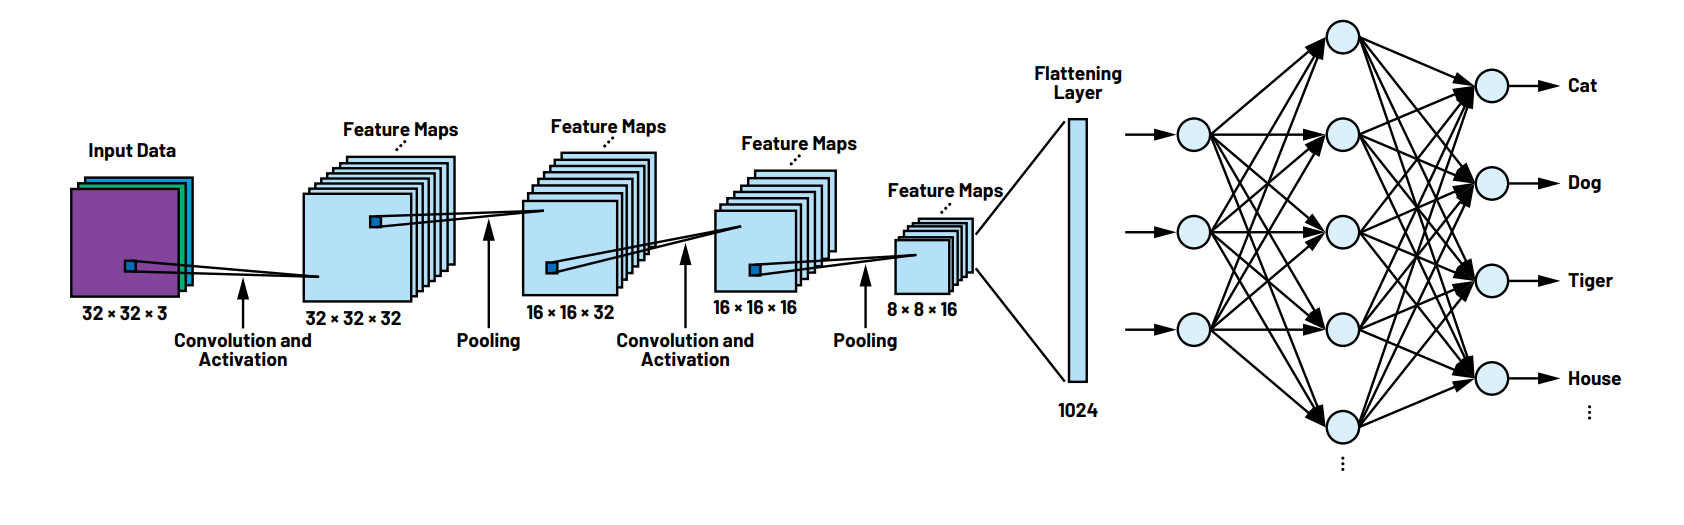
\includegraphics[width=1\textwidth]{Immagini/Screenshot 2026-10-18 153943.png}
\end{figure}

\subsection{Architettura generale}

Un'immagine viene rappresentata come un volume tridimensionale:
\[
X \in \mathbb{R}^{H \times W \times C_{\text{in}}},
\]
dove $H$ è l'altezza, $W$ la larghezza e $C_{\text{in}}$ il numero di
canali. Un'immagine RGB, ad esempio, possiede tre canali.

L'elaborazione segue generalmente questo schema:
\[
\text{Input}
\rightarrow \text{Convoluzione}
\rightarrow \text{Attivazione}
\rightarrow \text{Pooling}
\rightarrow \cdots
\rightarrow \text{Classificatore}.
\]

I primi livelli rilevano, colori e texture; i successivi riconosconoforme e parti
di oggetti. Infine il calssificatore prevedere la classe dell'immagine.

Ogni livello trasforma un volume di ingresso in un volume di uscita.
Alcuni livelli, come quelli convoluzionali, possiedono parametri
addestrabili; altri, come il pooling tradizionale, non hanno parametri
da apprendere.

\subsection{Operatori sulle immagini}

Nell'elaborazione tradizionale delle immagini si distinguono due
categorie principali di operatori:

\begin{itemize}
    \item \textbf{Operatori puntuali}: il valore di uscita di un pixel
    dipende esclusivamente dal corrispondente pixel di ingresso.
    \item \textbf{Operatori locali}: il valore di uscita dipende da una
    regione di pixel vicini. I filtri spaziali appartengono a questa
    categoria.
\end{itemize}

\subsection{Operatori lineari e invarianti per traslazione}

Una classe importante di operatori locali è costituita dagli operatori
LSI (\textit{Linear Shift-Invariant}), cioè lineari e invarianti per
traslazione.

La linearità richiede che, per due immagini $I_1$ e $I_2$ e due
costanti $a$ e $b$,
\[
T\{aI_1+bI_2\}=aT\{I_1\}+bT\{I_2\}.
\]

L'invarianza per traslazione richiede invece che traslare l'immagine
prima del filtraggio equivalga a traslare il risultato dopo il filtraggio:
\[
T\{SI\}=S\,T\{I\},
\]
dove $S$ indica un'operazione di traslazione.

QUINDI: il filtro si comporta allo stesso modo in tutte le posizioni
dell'immagine.

Un operatore LSI può essere descritto mediante un kernel(filtro), che puo' essere proggettato 
manualmente o appreso durante addestramento.


\subsection{Convoluzione}

La convoluzione applica un kernel all'immagine facendolo scorrere
nelle diverse posizioni. In ogni posizione, i valori della finestra
vengono moltiplicati per i corrispondenti pesi del kernel e i prodotti
vengono sommati.

Per un'immagine discreta $I$ e un kernel $K$, la convoluzione è definita
come:
\[
O(x,y)=
\sum_m\sum_n I(m,n)K(x-m,y-n).
\]

Nelle implementazioni delle CNN si utilizza comunemente la
\textit{cross-correlation}, spesso chiamata comunque convoluzione:
\[
O(i,j)=
\sum_m\sum_n I(i+m,j+n)K(m,n).
\]

La differenza consiste nel ribaltamento del kernel nelle due
direzioni. Per l'apprendimento dei filtri, entrambe le convenzioni
possono essere utilizzate in modo coerente.

\begin{figure}[htbp]
    \centering
    % Prima immagine a sinistra
    \begin{minipage}{0.45\textwidth}
        \centering
        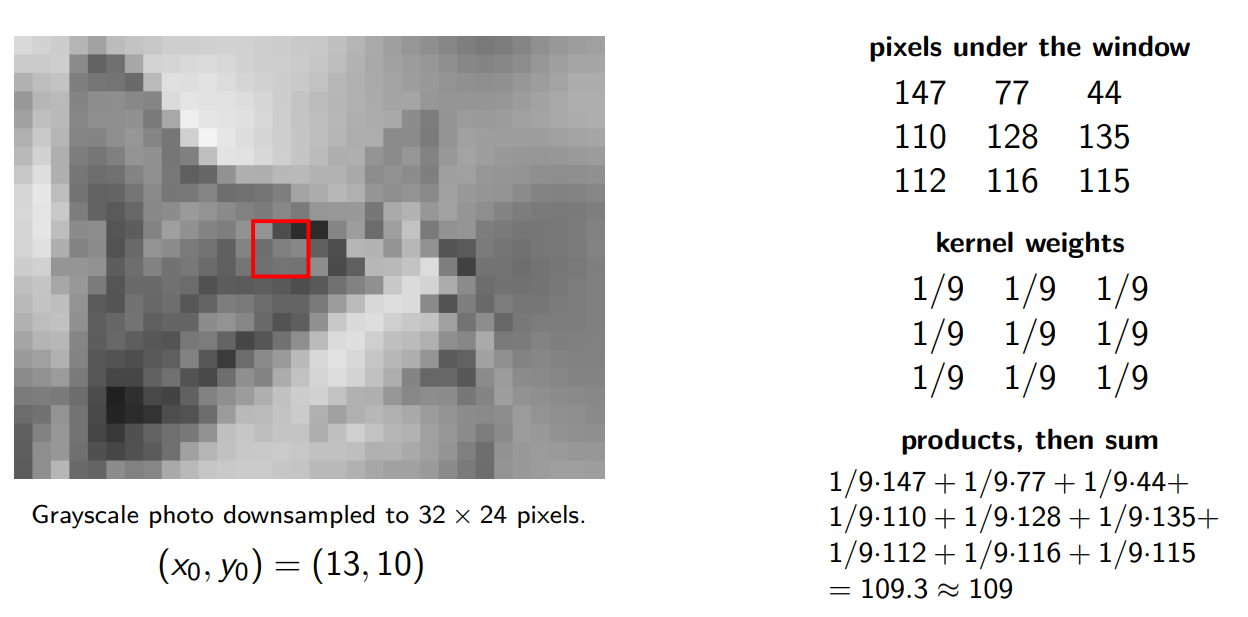
\includegraphics[width=\linewidth]{Immagini/gatto1.png}
    \end{minipage}\hfill
    % Seconda immagine a destra
    \begin{minipage}{0.45\textwidth}
        \centering
        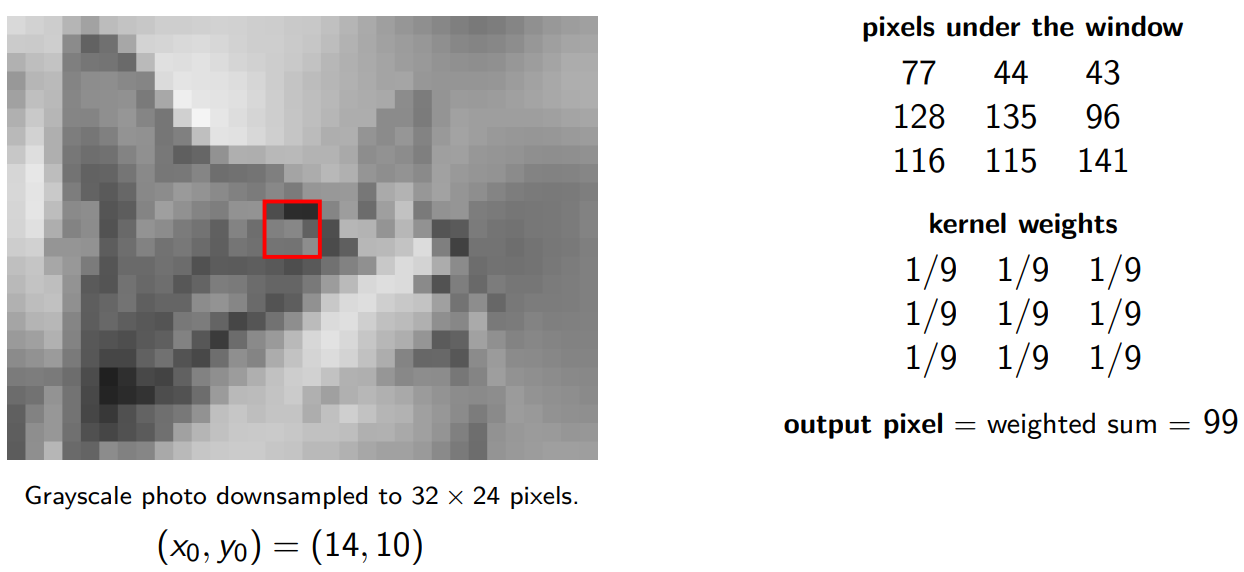
\includegraphics[width=\linewidth]{Immagini/gatto2.png}
    \end{minipage}
    \caption{Esempio di sliding 3X3}
\end{figure}

OSSERVAZIONE:
Senza padding, un filtro $3\times 3$ applicato a un'immagine
$32\times24$ con stride $1$ produce un'uscita di dimensioni
$30\times22$.

\subsection{Principi fondamentali delle CNN}

Le CNN si basano su due principi che le distinguono dai livelli completamente connessi.

\subsubsection{Condivisione dei pesi}
Il kernel utilizzato in tutto lo psazioe e' lo stesso (\textit{weight sharing}).

La condivisione dei pesi riduce il numero di parametri da apprendere e rende possibile
riutilizzare le caratteristiche in punti diversi dell'immagine.
\begin{figure}[htbp]
\centering
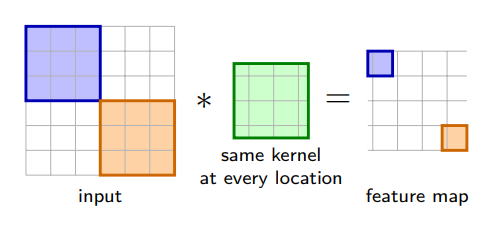
\includegraphics[width=0.5\textwidth]{Immagini/Screenshot 2026-10-18 160729.png}
\end{figure}

\subsubsection{Connettività sparsa}

Ogni neurone convoluzionale è collegato soltanto a una regione locale
dell'ingresso, anziché a tutti i pixel. Questa proprietà prende il nome
di \textit{sparse connectivity}.

La regione dell'ingresso che influenza il valore di un neurone è
chiamata \textit{campo recettivo} (\textit{receptive field}).
\begin{figure}[htbp]
\centering
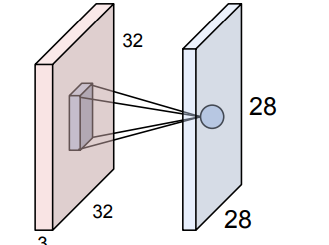
\includegraphics[width=0.3\textwidth]{Immagini/Screenshot 2026-10-18 160626.png}
\end{figure}


\subsection{Convoluzione con più canali}

Un'immagine RGB ha tre canali, quindi un filtro spaziale $3\times3$
deve possedere dimensioni complessive $3\times3\times3$.

In generale, se input ha $C_{\text{in}}$ canali, ogni filtro
possiede dimensioni:
\[
K\times K\times C_{\text{in}}.
\]

Il filtro applica un kernel a ciascun canale, somma i contributi
ottenuti e aggiunge un bias:
\[
F(i,j)=b+
\sum_{c=1}^{C_{\text{in}}}
\sum_m\sum_n
I(i+m,j+n,c)K_c(m,n).
\]

Ogni filtro produce una singola mappa bidimensionale delle
caratteristiche (\textit{feature map}).

Utilizzando $C_{\text{out}}$ filtri distinti (iperparametro), si ottengono
$C_{\text{out}}$ mappe, che vengono impilate lungo la dimensione
dei canali. Il volume di uscita ha quindi forma:
\[
H_{\text{out}}\times W_{\text{out}}\times C_{\text{out}}.
\]

\subsection{Iperparametri convoluzionali}

I principali iperparametri di un livello convoluzionale sono:
\begin{itemize}
    \item \textbf{Kernel size $K$}: dimensione spaziale del filtro;
    \item \textbf{Numero di filtri}: determina il numero di canali ($C_{\text{out}}$)
    dell'uscita;
    \item \textbf{Stride $S$}: passo con cui il filtro si sposta, più e' grande più la dimensione dell uscita
    sara' piccola;
    \item \textbf{Padding $P$}: valori aggiunti ai bordi dell'ingresso.
\end{itemize}

\subsubsection{Padding}

Il padding aggiunge valori attorno all'immagine prima della convoluzione.
Le modalità più comuni includono:
\begin{itemize}
    \item \textbf{Zero padding}: aggiunge valori pari a zero;
    \item \textbf{Reflect}: utilizza una riflessione dei valori ai bordi;
    \item \textbf{Replicate}: ripete i valori del bordo;
    \item \textbf{Circular}: utilizza valori provenienti dal bordo opposto.
\end{itemize}

OSSERVAZIONE:
Con \textit{valid} non si aggiunge padding e l'uscita si riduce.
Con \textit{same}, per kernel dispari e stride $1$, si sceglie il
padding in modo da conservare le dimensioni spaziali dell'ingresso.

\subsubsection{Calcolo delle dimensioni dell'uscita}

Per un ingresso di altezza $H_{\text{in}}$, kernel di dimensione $K$,
padding $P$ e stride $S$, l'altezza dell'uscita è:
\[
H_{\text{out}}=
\left\lfloor
\frac{H_{\text{in}}+2P-K}{S}
\right\rfloor+1.
\]

Analogamente, per la larghezza:
\[
W_{\text{out}}=
\left\lfloor
\frac{W_{\text{in}}+2P-K}{S}
\right\rfloor+1.
\]

% \paragraph{Esempio svolto.}

% Consideriamo un ingresso $7\times7$, un kernel $3\times3$ e
% nessun padding ($P=0$).

% Con stride $S=1$:
% \[
% H_{\text{out}}=
% \left\lfloor\frac{7-3}{1}\right\rfloor+1=5.
% \]
% L'uscita è quindi $5\times5$.

% Con stride $S=2$:
% \[
% H_{\text{out}}=
% \left\lfloor\frac{7-3}{2}\right\rfloor+1=3.
% \]
% L'uscita è quindi $3\times3$.

% Con stride $1$ e padding $P=1$:
% \[
% H_{\text{out}}=
% \left\lfloor\frac{7+2-3}{1}\right\rfloor+1=7.
% \]
% In questo caso le dimensioni spaziali vengono mantenute.

\subsubsection{Numero di parametri addestrabili}

Un livello convoluzionale con $C_{\text{out}}$ filtri, kernel
$K\times K$ e ingresso con $C_{\text{in}}$ canali possiede
\[
N_{\text{parametri}}=
(K^2C_{\text{in}})C_{\text{out}}+C_{\text{out}}.
\]

Il primo termine conta i pesi dei filtri; il secondo conta un bias
per ciascun filtro, se il bias è presente.

% \paragraph{Esempio svolto.}

% Consideriamo un'immagine RGB, quindi $C_{\text{in}}=3$, e un livello
% con 16 filtri $3\times3$. Il numero di parametri è:
% \[
% \begin{aligned}
% N_{\text{parametri}}
% &=(3\cdot3\cdot3)\cdot16+16\\
% &=432+16\\
% &=448.
% \end{aligned}
% \]

% Il livello possiede quindi 448 parametri addestrabili. Il numero non
% dipende dall'altezza o dalla larghezza dell'immagine, perché i pesi
% sono condivisi tra le diverse posizioni.

\subsection{Filtri appresi e mappe delle attivazioni}

Durante l'addestramento, i pesi dei filtri vengono aggiornati
attraverso la (\textit{backpropagation})e un algoritmo di ottimizzazione.

\begin{figure}[htbp]
\centering
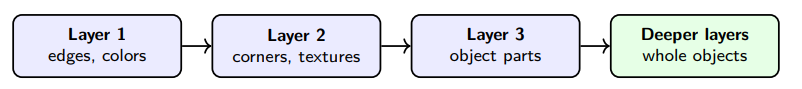
\includegraphics[width=0.7\textwidth]{Immagini/Screenshot 2026-10-18 172745.png}
\end{figure}
Ogni strato combina i modelli di quello precedente: bordi → forme → parti → oggetti

Una \textit{activation map} o \textit{feature map} mostra la risposta
di un filtro nelle diverse posizioni dell'immagine.

\subsection{Funzioni di attivazione}

Le funzioni di attivazione introducono non linearità nella rete.
Senza di esse, la composizione di più livelli lineari sarebbe
equivalente a un'unica trasformazione lineare:
\[
W_2(W_1x)=(W_2W_1)x.
\]
Di conseguenza, aumentare il numero di livelli non permetterebbe
di rappresentare funzioni non lineari più complesse.

\subsubsection{ReLU in CNN}
La funzione ReLU (\textit{Rectified Linear Unit}) è  la piu utilizzata nelle CNN:
\[
f(x)=\max(0,x)=
\begin{cases}
0, & x\leq 0,\\
x, & x>0.
\end{cases}
\]

Vantaggi
\begin{itemize}
  \item Convergenza accelerata
  \item Efficienza computazionale
\end{itemize}

Probelma della ReLU:
Per $x<0$ il gradiente è zero. Un neurone che rimane sempre in
questa regione può smettere di apprendere: questo problema è noto
come \textit{dying ReLU}.

\subsubsection{Leaky ReLU ed ELU}

La Leaky ReLU mantiene una piccola pendenza per gli input negativi:
\[
f(x)=\max(x,\alpha x),
\qquad \alpha>0.
\]

Per esempio, con $\alpha=0.01$:
\[
f(-2)=\max(-2,-0.02)=-0.02.
\]

La funzione ELU è definita come:
\[
f(x)=
\begin{cases}
x, & x>0,\\
\alpha(e^x-1), & x\leq0.
\end{cases}
\]

Per valori negativi, ELU produce valori che si avvicinano a
$-\alpha$ quando $x$ tende a $-\infty$. Entrambe le funzioni
modificano il comportamento della ReLU per gli input negativi.

\begin{figure}[H]
\centering
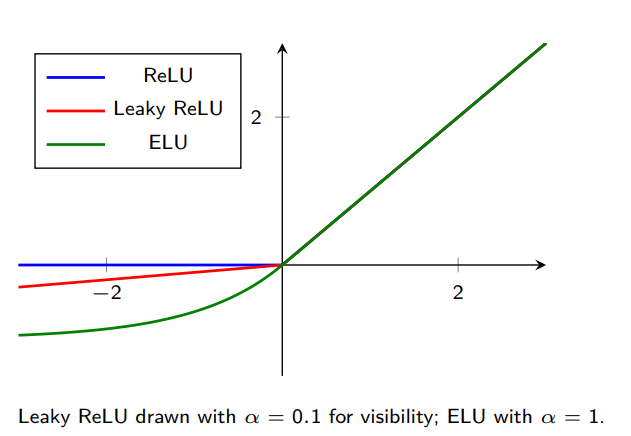
\includegraphics[width=0.5\textwidth]{Immagini/Screenshot 2026-10-18 173702.png}
\end{figure}

\subsection{Livelli di pooling}

Il pooling riduce le dimensioni spaziali delle mappe e viene 
applicato separatamente a ciascun canale.

I suoi iperparametri principali sono:
\begin{itemize}
    \item $K$: Dimensione della finestra di pooling;
    \item $S$: Pixel di shift della finestra;
\end{itemize}

Se la dimensione della finestra coincide con lo stride, le finestre
non si sovrappongono.
\begin{figure}[H]
\centering
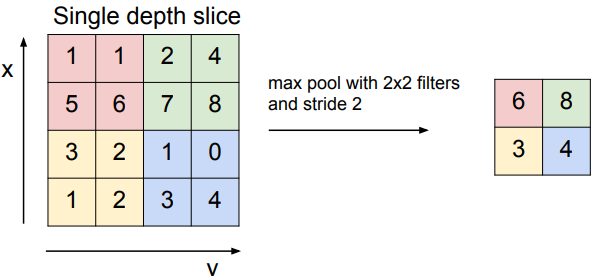
\includegraphics[width=0.5\textwidth]{Immagini/Screenshot 2026-10-18 180401.png}
\end{figure}

\subsubsection{Funzione di aggregazione}
\begin{itemize}
  \item Max Pooling: seleziona il valore massimo di ciascuna finestra
  \item Average Pooling: sostituisce ogni finestra con la media dei suoi valori
\end{itemize}

\textit{VANTAGGI}:
\begin{itemize}[label=\textbullet]
    \item \textbf{Invarianza spaziale:} Aumentano la robustezza rispetto all'esatta posizione spaziale delle \textit{feature}.
    \item \textbf{Efficienza:} Riducono drasticamente il costo computazionale e l'occupazione di memoria.
    \item \textbf{Regolarizzazione:} Aiutano a prevenire l'overfitting riducendo le dimensioni spaziali dell'input.
    \item \textbf{Campo ricettivo:} Aumentano il \textit{receptive field} dei layer successivi.
\end{itemize}


\subsection{Classificatore finale}

Dopo i livelli convoluzionali, le mappe delle caratteristiche
vengono trasformate in una rappresentazione adatta alla
classificazione.

\begin{figure}[H]
\centering
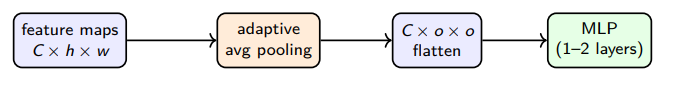
\includegraphics[width=0.6\textwidth]{Immagini/Screenshot 2026-10-18 180422.png}
\end{figure}

L'\textit{Adaptive Average Pooling} produce mappe con una dimensione
spaziale prestabilita, indipendentemente dalla dimensione spaziale
iniziale compatibile con il livello.

Il \textit{Flatten} trasforma il volume in un vettore. Per esempio,
un volume $8\times8\times16$ diventa un vettore di dimensione:
\[
8\cdot8\cdot16=1024.
\]

Il vettore viene fornito alla MLP (\textit{Multi-Layer Perceptron}),
che utilizza livelli completamente connessi per produrre la
predizione finale.

\section{Classiche Architetture}

\subsection{LeNet-5}

LeNet-5 è una delle prime CNN \textit{end-to-end}, per compiti
come il riconoscimento di cifre scritte a mano.

\begin{figure}[H]
\centering
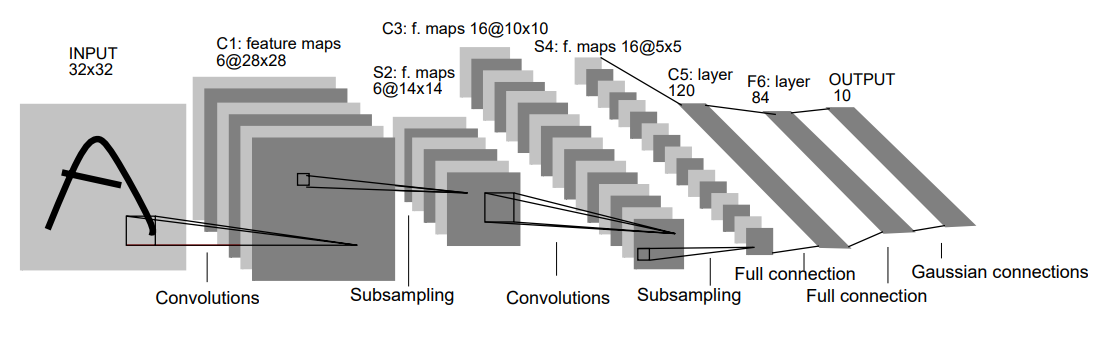
\includegraphics[width=0.6\textwidth]{Immagini/Screenshot 2026-10-19 161923.png}
\caption{5x5 Kernel, avarage pooling(2x2 windows with stride 2), Singmoid}
\end{figure}

\subsection{AlexNet}
È caratterizzata da un'architettura profonda a 8 livelli 
(5 convoluzionali, 3 \textit{fully connected}) ed è stata pioniera 
nell'uso delle funzioni di attivazione ReLU e della parallelizzazione su due GPU.

\begin{figure}[H]
\centering
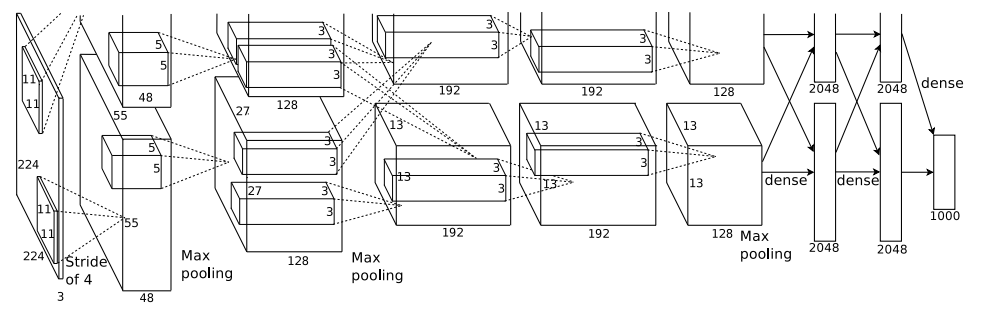
\includegraphics[width=0.8\textwidth]{Immagini/Screenshot 2026-10-19 162813.png} 
\caption{11x11 First Kernel, ReLU Activation, 2-GPU Parallelization}
\end{figure}

\subsection{VGG-16}

LA VGG si basa su un'architettura semplice e modulare:

\begin{itemize}
    \item \textbf{Principio:} Sostituire pochi livelli con kernel grandi con molti 
    livelli con kernel piccoli e costanti ($3 \times 3$).
    \item \textbf{Vantaggi dei filtri piccoli:} 
    \begin{itemize}
        \item Tre livelli $3 \times 3$ hanno lo stesso \textit{receptive field} di un singolo livello $7 \times 7$.
        \item Maggiore non-linearità (tre attivazioni ReLU invece di una).
        \item Minor numero di parametri nei livelli convoluzionali.
    \end{itemize}
    \item \textbf{Caratteristiche tecniche:}
    \begin{itemize}
        \item Input: Immagini RGB $224 \times 224$.
        \item Convoluzioni: Kernel $3 \times 3$ con \textit{stride} 1.
        \item Pooling: $2 \times 2$ Max-Pooling con \textit{stride} 2.
        \item Attivazione: ReLU dopo ogni livello convoluzionale e \textit{fully connected}.
    \end{itemize}
    
    \begin{figure}[H]
    \centering
    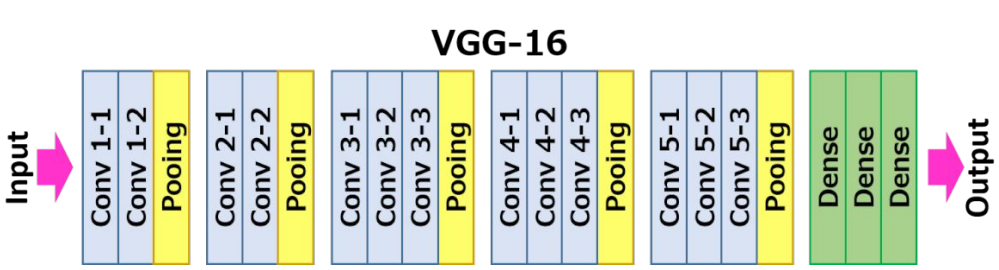
\includegraphics[width=0.8\textwidth]{Immagini/Screenshot 2026-10-19 163756.png} 
    \caption{Constant $3 \times 3$ Kernels, $2 \times 2$ Max-Pooling (stride 2), ReLU Activations}
    \end{figure}

    \item \textbf{Limiti (Degradazione delle prestazioni):} Aumentare eccessivamente la profondità porta a un calo delle 
    prestazioni sia in addestramento che in test. Questo non è dovuto all'overfitting, 
    ma probabilmente al problema del \textit{vanishing/exploding gradient} 
    (i gradienti diventano troppo piccoli o troppo grandi, bloccando l'addestramento).
\end{itemize}

\subsection{ResNet (Residual Networks)}

Risolve il limite della VGG-16.

\begin{itemize}
    \item \textbf{La Soluzione (Residual Learning):} Invece di costringere un blocco di layer a imparare 
    l'intera mappatura $H(x)$, gli si fa imparare solo la differenza/residuo $F(x)$. L'output finale diventa $H(x) = F(x) + x$.
    \begin{figure}[H]
    \centering
    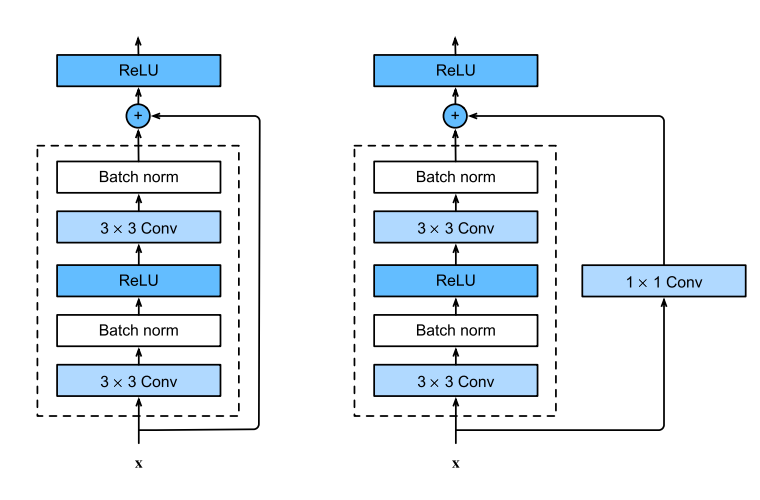
\includegraphics[width=0.5\textwidth]{Immagini/Screenshot 2026-10-19 165619.png} 
    \caption{Building block della ResNet: l'input $x$ salta i layer e si somma all'output $F(x)$.}
    \end{figure}

    \item \textbf{Skip Connections (Residual Block):}
    \begin{itemize}
        \item L'input $x$ "salta" i layer convoluzionali e viene sommato direttamente al loro output.
        \item Se i layer in più non servono, la rete impara semplicemente ad azzerare i pesi del blocco 
        ($F(x) = 0$), lasciando passare intatto l'input $x$.
        \item Questo "ponte" permette al gradiente di fluire all'indietro senza svanire,
         risolvendo il blocco matematico della VGG.
    \end{itemize}
    \item \textbf{Impatto e differenze con VGG:}
    \begin{itemize}
        \item la ResNet arriva fino a 152 layer.
        \item Miglioramento performance e prevenzione della degradazione delle performance con \textit{skip connections}
    \end{itemize}
\end{itemize}

\begin{figure}[H]
\centering
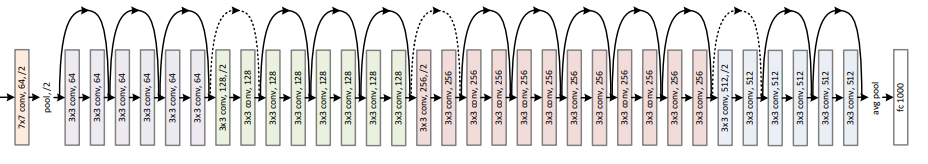
\includegraphics[width=0.9\textwidth]{Immagini/Screenshot 2026-10-19 165638.png} 
\end{figure}

\subsection{Batch Normalization}

Tecnica introdotta per stabilizzare e accelerare l'addestramento delle reti neurali profonde.

\begin{itemize}
    \item \textbf{Il Problema (Internal Covariate Shift):} Durante l'addestramento, l'aggiornamento dei 
    pesi di un livello modifica la distribuzione delle attivazioni che passano al livello successivo. 
    Ogni livello si ritrova a dover rincorrere un "bersaglio mobile", rallentando l'addestramento.
    \begin{figure}[H]
    \centering
    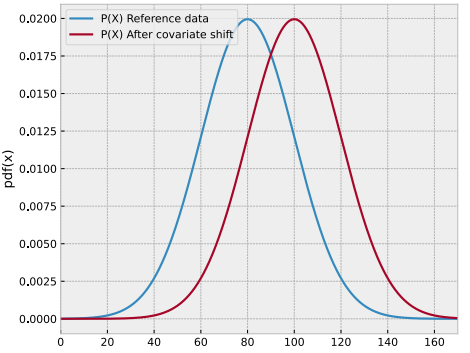
\includegraphics[width=0.5\textwidth]{Immagini/Screenshot 2026-10-19 170343.png} 
    \end{figure}

    \item \textbf{La Soluzione:} Standardizzare (forzare media nulla e varianza unitaria) gli input di ogni
     livello basandosi sui dati dell'attuale \textit{mini-batch}.
      \begin{figure}[H]
      \centering
      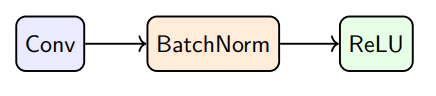
\includegraphics[width=0.5\textwidth]{Immagini/Screenshot 2026-10-19 170350.png} 
      \end{figure}
    
    \item \textbf{Funzionamento in Addestramento (Training):}
    \begin{enumerate}
        \item \textbf{Media del mini-batch:} $\mu_B = \frac{1}{m} \sum_{i=1}^{m} x_i$
        \item \textbf{Varianza del mini-batch:} $\sigma^2_B = \frac{1}{m} \sum_{i=1}^{m} (x_i - \mu_B)^2$
        \item \textbf{Normalizzazione:} $\hat{x}_i = \frac{x_i - \mu_B}{\sqrt{\sigma^2_B + \epsilon}}$ 
        \quad (\textit{$\epsilon$ evita la divisione per zero})
        \item \textbf{Scale and Shift:} $y_i = \gamma \hat{x}_i + \beta$
    \end{enumerate}
    
    \item \textbf{Parametri Apprendibili ($\gamma$ e $\beta$):} Forzare media 0 e varianza 1 limita da rete.
    I parametri $\gamma$ (scala) e $\beta$ (spostamento) vengono imparati durante il training
    
    \item \textbf{Funzionamento in Inferenza (Test):} In fase di predizione, il \textit{mini-batch} 
    potrebbe essere di un solo elemento, rendendo impossibile il calcolo statistico. 
    Si utilizzano quindi la \textbf{media e varianza dell'intera popolazione} 
    (calcolate come \textit{moving average} durante il training). La formula diventa deterministica:
    \[ \hat{x} = \frac{x - \mu_{pop}}{\sqrt{\sigma^2_{pop} + \epsilon}} \]
    
    \item \textbf{Vantaggi:}
    \begin{itemize}
        \item \textbf{Training più veloce:} Uso di \textit{learning rate} molto più alti.
        \item \textbf{Meno sensibilità all'inizializzazione:} Rete più robusta ai pesi di partenza.
        \item \textbf{Regolarizzazione implicita:} Il rumore introdotto dal singolo mini-batch agisce da 
        leggero regolarizzatore (Meno utilizzo del Dropout).
    \end{itemize}
\end{itemize}

\section{Serie Temporali}
I dati in sequenza, come meteo, trading o frasi, hanno un ordine che conta.
Un MLP non va bene: ha un numero fisso di input e non tiene conto dell'ordine

\subsection{Definizione}
\begin{itemize}
  \item Una serie temporale è un insieme di osservazioni $\{x_t\}_{t\in\tau}$ raccolte nel tempo,
  dove l'ordine conta.
  \item In base a $\tau$ si distingue tra:
  \begin{itemize}
    \item \textbf{Continua}: le osservazioni sono fatte in modo continuo;
    \item \textbf{Discreta}(Piu' comune): le osservazioni sono in numero finito. Se la distanza temporale tra 
    due punti è fissa, la serie è \textit{campionata} con frequenza di campionamento $f_c$.
  \end{itemize}
\end{itemize}

\begin{figure}[H]
\centering
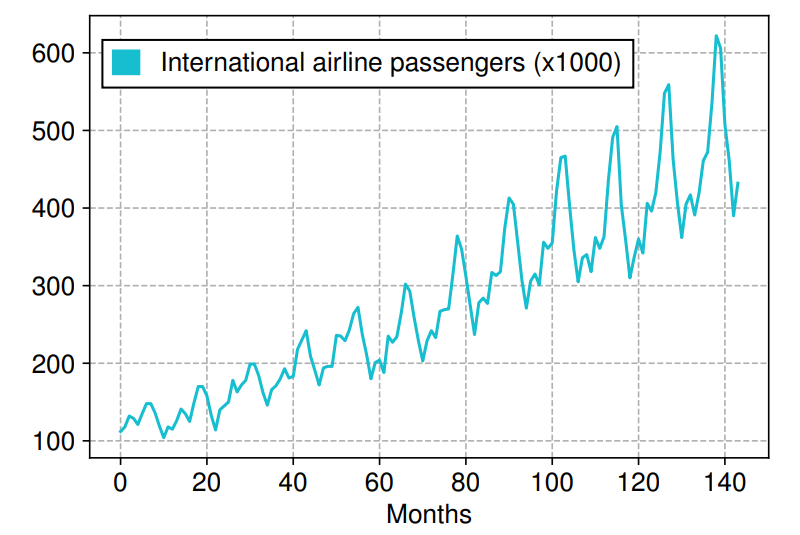
\includegraphics[width=0.6\textwidth]{Immagini/Screenshot 2026-10-20 165705.png} 
\caption{Serie discreta e $f_c$ costante}
\end{figure}

\subsection{Caratteristiche ricorrenti}
\begin{description}
  \item\textbf{Trend:} Direzione finale della serie(Es: Passeggeri in aumento)
  \item\textbf{Stagionalit:} Schema che si ripete a ogni periodo di riferimento(ES:Picco ogni estate)
  \item\textbf{Ciclico:} Oscillazione periodica attorno al trend.
  \item\textbf{Outlier:} Valore anomalo rispetto agli altri.
  \item\textbf{Stazionarietà:} La serie è stazionaria se media e varianza non cambiano nel tempo.
\end{description}

\section{Forecasting}
Se osservata una serie su un periodo $\tau$, si vuole stimare un valore futuro $\hat{x}_{\tau+h}$ con $h>0$.
Il valore $h$ è l'\emph{orizzonte di previsione}.

QUINDI: Il forecasting si usa per fare previsioni basate sul passato.

Nel grafico la previsione non è un solo valore: attorno alla linea c'è un intervallo di valori,
e ogni valore ha una percentuale di uscita (una probabilità)
\begin{figure}[H]
\centering
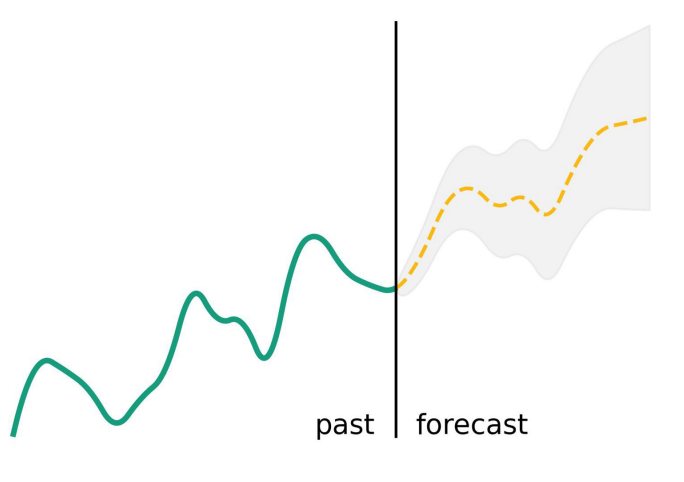
\includegraphics[width=0.4\textwidth]{Immagini/Screenshot 2026-10-20 171203.png} 
\caption{Usato in ambito di finanza, eneriga, Retail, ecc..}
\end{figure}

\subsection{Modello AutoRegressivo AR($p$)}
\[
  x_t = \sum_{i=1}^{p} \phi_i\, x_{t-i} + \xi_t
\]
$x_t$ è il nuovo valore. Si ottiene come trasformazione lineare dei $p$ valori passati,
più una variazione casuale detta \emph{rumore bianco}.
\begin{itemize}
  \item $\phi_i$ sono i parametri apprendibili.
  \item $\xi_t$ è di solito modellato come una normale a media 0.
\end{itemize}

\subsection{Preparazione dei dati}
I dati di una serie temporale non possono essere trattati semplicemente come un normale dataset, 
perché l'informazione temporale è fondamentale.

Alcune variabili temporali sono cicliche: dopo un certo intervallo, i loro valori ricominciano da capo.
(ES: mesi dell'anno, da 1 a 12)

Per preservare la periodicità, una variabile ciclica può essere rappresentata mediante seno e coseno:

\[
\operatorname{Sin}(\text{hour})
=
\sin\left(\text{hour}\cdot\frac{2\pi}{24}\right)
\]

\[
\operatorname{Cos}(\text{hour})
=
\cos\left(\text{hour}\cdot\frac{2\pi}{24}\right)
\]

\section{Recurrent Neural Networks RNNs}

\subsection{Introduzione}

Nelle reti neurali ricorrenti, sono presenti connessioni tra i vari step di esecuzione, le 
 informazioni vengono mantenute e utilizzate.

Le \textbf{Recurrent Neural Networks (RNN)} sono reti neurali specializzate nell'
elaborazione di sequenze, come serie temporali e sequenze di parole.

Rispetto alle reti feedforward, possono gestire sequenze in tutte le fasi.
\begin{figure}[H]
\centering
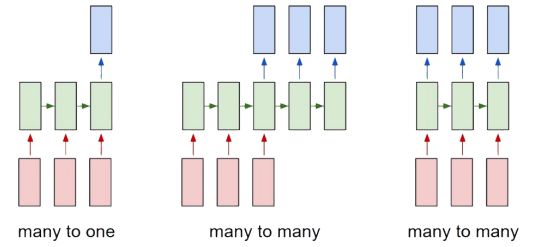
\includegraphics[width=0.4\textwidth]{Immagini/Screenshot 2026-10-20 181118.png} 
\end{figure}

\subsection{Vanilla RNN}

La \textit{vanilla RNN} è la forma più semplice di rete neurale ricorrente e utilizza tre 
insiemi di parametri:

\begin{itemize}
    \item $U$: trasforma l'input nello stato nascosto (Trasformazione lineare);
    \item $W$: parametrizza la transizione tra stati nascosti consecutivi;
    \item $V$: trasforma lo stato nascosto nell'output.
\end{itemize}

Le equazioni del modello sono:

\noindent
\begin{minipage}{0.5\textwidth}
    \centering
    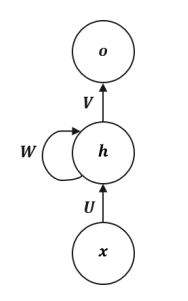
\includegraphics[width=0.4\linewidth]{Immagini/Screenshot 2026-10-20 181126.png}
\end{minipage}
\begin{minipage}{0.5\textwidth}
    \[
    \begin{cases}
    h^{(t)} = \phi\left(Wh^{(t-1)} + Ux^{(t)}\right)\\[4pt]
    o^{(t)} = Vh^{(t)}
    \end{cases}
    \]
\end{minipage}

dove:
\begin{itemize}
    \item $x^{(t)}$ è l'input al tempo $t$;
    \item $h^{(t-1)}$ è lo stato nascosto precedente;
    \item $h^{(t)}$ è il nuovo stato nascosto;
    \item $\phi$ è la funzione di attivazione;
    \item $o^{(t)}$ è l'output al tempo $t$.
\end{itemize}

Il nuovo stato nascosto $h^{(t)}$ dipende sia dall'input corrente sia dallo stato precedente, e lo possiamo considerare 
come \textbf{sintesi delle informazioni rilevanti degli input precedenti} con una perdita di informazioni;

In questo modo, la rete può utilizzare informazioni provenienti dai passi temporali precedenti.

\subsection{Addestramento di una RNN}

Srotolando il ciclo nascosto, otteniamo una sequenza di operazioni con struttura ripetut:
\[
h^{(t)} = f\left(h^{(t-1)},x^{(t)};\theta\right)
\]
\begin{figure}[H]
\centering
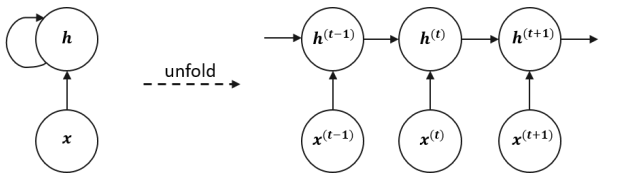
\includegraphics[width=0.6\textwidth]{Immagini/Screenshot 2026-10-20 181134.png} 
\end{figure}

dove $\theta$ rappresenta i parametri della rete.

Lo srotolamento permette di rappresentare la rete come un grafo computazionale aciclico diretto (DAG), 
sul quale è possibile applicare la backpropagation.

\subsection{Backpropagation Through Time (BPTT)}

Nelle RNNs, il gradiente si propaga all'indietro nei diversi step temporali \textbf{Backpropagation Through Time (BPTT)}.

Consideriamo una rete che elabora una sequenza di lunghezza $\tau=3$ 
\begin{figure}[H]
\centering
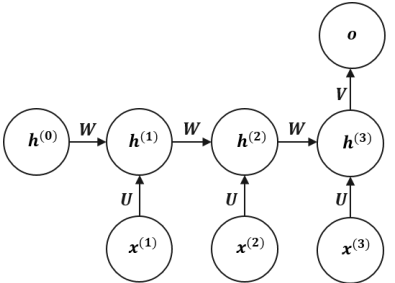
\includegraphics[width=0.4\textwidth]{Immagini/Screenshot 2026-10-20 185108.png} 
\end{figure}

Indicando con $\mathcal{L}$ la funzione di perdita, i parametri $V$, $W$ e $U$ 
vengono aggiornati utilizzando i rispettivi gradienti.

Il gradiente rispetto a $V$ dipende dall'output corrente:

\[
\frac{\partial \mathcal{L}}{\partial V}
=
\frac{\partial \mathcal{L}}{\partial o}
\frac{\partial o}{\partial V}
\]

I gradienti rispetto a $W$ e $U$, invece, dipendono anche dagli stati nascosti precedenti:

\[
\frac{\partial \mathcal{L}}{\partial W}
=
\frac{\partial \mathcal{L}}{\partial o}
\frac{\partial o}{\partial h^{(3)}}
\sum_{k=0}^{3}
\left(
\frac{\partial h^{(3)}}{\partial h^{(k)}}
\frac{\partial h^{(k)}}{\partial W}
\right)
\]

\[
\frac{\partial \mathcal{L}}{\partial U}
=
\frac{\partial \mathcal{L}}{\partial o}
\frac{\partial o}{\partial h^{(3)}}
\sum_{k=0}^{3}
\left(
\frac{\partial h^{(3)}}{\partial h^{(k)}}
\frac{\partial h^{(k)}}{\partial U}
\right)
\]

QUINDI: Apprendimento dei parametri ricorrenti dipende dai contributi dei diversi passi temporali.

\subsection{Problema delle dipendenze a lungo termine}

Durante la BPTT, alcuni gradienti vengono calcolati applicando ripetutamente la chain rule.

Ad esempio:

\[
\frac{\partial h^{(3)}}{\partial h^{(1)}}
=
\frac{\partial h^{(3)}}{\partial h^{(2)}}
\frac{\partial h^{(2)}}{\partial h^{(1)}}
\]

Quando la sequenza è lunga, la moltiplicazione ripetuta di queste derivate può causare due problemi.

\begin{itemize}
    \item \textbf{Vanishing gradient:} i gradienti diventano progressivamente più piccoli, fino ad avvicinarsi a zero.
     Le informazioni provenienti da passi temporali lontani contribuiscono sempre meno all'apprendimento, 
     rendendo difficile imparare dipendenze a lungo termine.

    \item \textbf{Exploding gradient:} i gradienti diventano progressivamente più grandi, 
    causando problemi numerici e compromettendo l'ottimizzazione.
\end{itemize}

Con le funzioni di attivazione $\tanh$ e sigmoide, puo' favorire il vanishing gradient.

Entrambi i problemi possono essere mitigati mediante:
\begin{itemize}
    \item inizializzazione appropriata dei pesi;
    \item scelta accurata delle funzioni di attivazione;
    \item \emph{gradient clipping}.
\end{itemize}

\subsection{Architetture ricorrenti avanzate}

introdotte reti con meccanismi di \textit{gating apprendibili}, che controllona il flusso delle informazioni della rete
per affrontare  flusso dei gradienti e facilitare l'apprendimento a lungo termine:

\begin{itemize}
    \item \textbf{Long Short-Term Memory (LSTM)};
    \item \textbf{Gated Recurrent Unit (GRU)}.
\end{itemize}


\subsection{Long Short-Term Memory (LSTM)}

\begin{figure}[H]
\centering
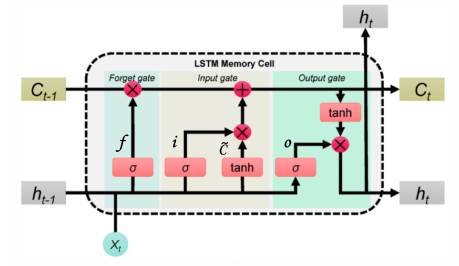
\includegraphics[width=0.6\textwidth]{Immagini/Screenshot 2026-10-20 181202.png} 
\end{figure}

Le equazioni di aggiornamento sono:

\[
\begin{aligned}
i &= \sigma\left(x^{(t)}U_i+h^{(t-1)}W_i\right)\\
f &= \sigma\left(x^{(t)}U_f+h^{(t-1)}W_f\right)\\
o &= \sigma\left(x^{(t)}U_o+h^{(t-1)}W_o\right)\\
\widetilde{C} &=
\tanh\left(x^{(t)}U_C+h^{(t-1)}W_C\right)\\
C^{(t)} &= C^{(t-1)}\odot f+\widetilde{C}\odot i\\
h^{(t)} &= \tanh\left(C^{(t)}\right)\odot o
\end{aligned}
\]

dove $\odot$ indica il prodotto elemento per elemento.

\subsubsection{Input, forget e output gate}

Le prime tre equazioni definiscono i tre gate della LSTM:

\begin{itemize}
    \item \textbf{Input gate $i$:} controlla quanta parte del nuovo contenuto candidato viene inserita nella memoria.
    \item \textbf{Forget gate $f$:} controlla quanta informazione della memoria precedente viene conservata.
    \item \textbf{Output gate $o$:} controlla quanta informazione dello stato interno viene esposta nell'output.
\end{itemize}

I gate hanno la stessa dimensione dello stato nascosto. Grazie alla funzione sigmoide $\sigma$, i loro valori sono compresi tra 0 e 1 e 
agiscono come interruttori continui e differenziabili.

\subsubsection{Stato candidato}

Lo stato candidato è calcolato come:

\[
\widetilde{C}
=
\tanh\left(x^{(t)}U_C+h^{(t-1)}W_C\right)
\]

Esso rappresenta il nuovo contenuto che potrebbe essere inserito nella memoria della rete.

L'input gate $i$ controlla quanto di questo contenuto viene effettivamente utilizzato.

\subsubsection{Aggiornamento della memoria}

La memoria viene aggiornata mediante:

\[
C^{(t)}
=
C^{(t-1)}\odot f
+
\widetilde{C}\odot i
\]

Il primo termine conserva una parte della memoria precedente, selezionata dal forget gate. Il secondo aggiunge il nuovo contenuto candidato, 
controllato dall'input gate.

L'output viene poi calcolato come:

\[
h^{(t)}
=
\tanh\left(C^{(t)}\right)\odot o
\]

La funzione $\tanh$ trasforma la memoria corrente, mentre l'output gate regola quanta informazione viene resa disponibile agli strati successivi.

\subsubsection{Stato della cella e stato nascosto}

La LSTM possiede due stati interni distinti:

\begin{itemize}
    \item \textbf{Cell state $C$:} rappresenta la memoria a lungo termine. Può conservare informazioni provenienti dai passi precedenti senza che 
    vengano sovrascritte rapidamente.

    \item \textbf{Hidden state $h$:} rappresenta la memoria a breve termine e funge anche da output. Cambia più frequentemente e contiene le
     informazioni utili per la previsione al passo corrente.
\end{itemize}

La distinzione tra memoria a lungo termine e stato nascosto permette alla LSTM di controllare meglio quali informazioni conservare e quali 
utilizzare per produrre l'output.




\section{Temporal Convolutional Networks}
Un modello di sequenza prende in input una sequenza di elementi (parole, lettere, serie temporali, segnali audio) e 
restituisce un elemento oppure un'altra sequenza. Alcuni compiti sono traduzione automatica,
forecasting e riassunto di testi. 

\subsection{Convoluzione 1D}

La Conv2D usata sulle immagini fa scorrere il kernel su due dimensioni. Nella \textbf{Conv1D} il kernel scorre in un'unica dimensione,
 il \textit{tempo}. Si applica a serie temporali e a testo, perché ogni istante o parola è rappresentato da un vettore 
di dimensione fissa (embedding).

La convoluzione discreta 1D è definita come
\[
(\mathbf{x} * \omega)(n) = \sum_{i=0}^{k-1} \mathbf{x}(n-i)\,\omega(i),
\]
dove $\mathbf{x}$ è la sequenza in intput di lunghezza $n$ e $\omega$ il kernel di lunghezza $k$(arbitraria).

Se ogni elemento ha $d$ feature, il kernel è una matrice $k \times d$: copre $k$ elementi consecutivi e, per ciascuno, tutte le feature. 
Ogni posizione produce \textbf{un solo numero}.

\paragraph{Esempio.} Frase di 7 parole, ciascuna con embedding di dimensione 4, e kernel $3 \times 4$.

\begin{center}
% Riga superiore: Input -> Freccia -> Output
\begin{minipage}{0.45\textwidth}
\centering
\textbf{Input} \\
\vspace{0.2cm}
\begin{tabular}{|l|c|c|c|c|}
\hline
Asimov & 0.2 & 0.1 & -0.3 & 0.4 \\ \hline
scrisse & 0.5 & 0.2 & -0.3 & -0.1 \\ \hline
molti & -0.1 & -0.3 & -0.2 & 0.4 \\ \hline
racconti & 0.3 & -0.3 & 0.1 & 0.1 \\ \hline
sui & 0.2 & -0.3 & 0.4 & 0.2 \\ \hline
robot & 0.1 & 0.2 & -0.1 & -0.1 \\ \hline
positronici & -0.4 & -0.4 & 0.2 & 0.3 \\ \hline
\end{tabular}
\end{minipage}%
\begin{minipage}{0.1\textwidth}
\centering
\Huge $\Rightarrow$
\end{minipage}%
\begin{minipage}{0.45\textwidth}
\centering
\textbf{Output} \\
\vspace{0.2cm}
\begin{tabular}{|l|c|}
\hline
Asimov scrisse molti & -1 \\ \hline
scrisse molti racconti & -0.5 \\ \hline
molti racconti sui & -3.6 \\ \hline
racconti sui robot & -0.2 \\ \hline
sui robot positronici & 0.3 \\ \hline
\end{tabular}
\end{minipage}

\vspace{0.8cm}

% Riga inferiore: Kernel
\textbf{Kernel ($3 \times 4$)} \\
\vspace{0.2cm}
\begin{tabular}{|c|c|c|c|}
\hline
3 & 1 & 2 & -3 \\ \hline
-1 & 2 & 1 & -3 \\ \hline
1 & 1 & -1 & 1 \\ \hline
\end{tabular}
\end{center}

\vspace{0.5cm}

Per la prima finestra (Asimov, scrisse, molti), si moltiplica il kernel con i valori corrispondenti elemento per elemento e si somma:
\[
(0.6+0.1-0.6-1.2) + (-0.5+0.4-0.3+0.3) + (-0.1-0.3+0.2+0.4) = -1.1 - 0.1 + 0.2 = -1.0 .
\]

\textbf{QUINDI:} il kernel è $3\times 4$ perché copre 3 parole e tutte le 4 feature di ciascuna.

\subsection{Convoluzione dilatata}

Per avere un campo recettivo ampio servirebbe una rete molto profonda oppure un filtro molto grande. La \textbf{convoluzione dilatata} 
lascia dei salti tra gli elementi del kernel, senza aumentare il numero di parametri:
\[
(\mathbf{x} * \omega)(n) = \sum_{i=0}^{k-1} \mathbf{x}(n-d\cdot i)\,\omega(i),
\]
dove $d$ è il fattore di dilatazione ($d=1$ dà la convoluzione normale).

\begin{figure}[H]
\centering
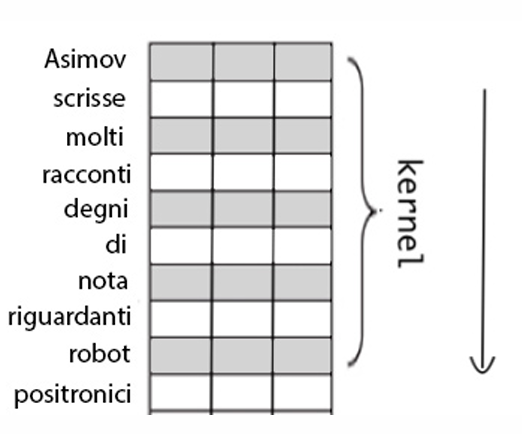
\includegraphics[width=0.4\textwidth]{Immagini/Screenshot 2026-10-24 185609.png} 
\end{figure}



\subsection{Convoluzione causale}

Una convoluzione standard può usare input futuri per calcolare l'uscita corrente, cosa non voluta nel forecasting.
Una \textbf{convoluzione causale} garantisce che l'uscita al tempo $t$ dipenda solo dagli input con tempo $\le t$.

\begin{figure}[H]
\centering
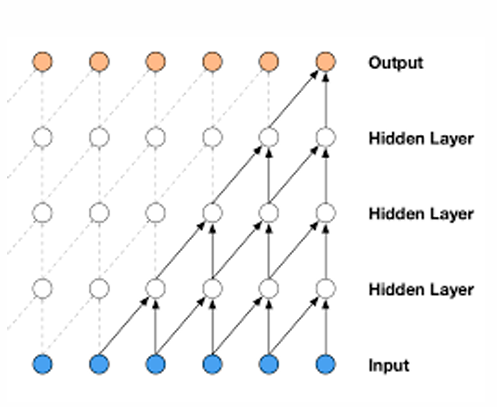
\includegraphics[width=0.4\textwidth]{Immagini/Screenshot 2026-10-24 185554.png} 
\end{figure}



\subsection{Temporal Convolutional Network (TCN)}
La TCN è composta da blocchi residuali di convoluzioni causali dilatate.

\begin{figure}[H]
\centering
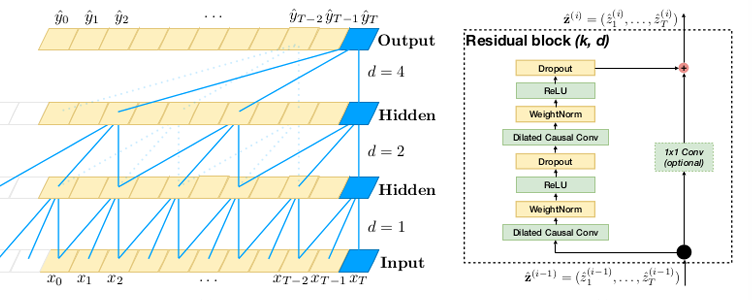
\includegraphics[width=0.6\textwidth]{Immagini/Screenshot 2026-10-24 190105.png} 
\end{figure}

Ogni blocco contiene due volte la sequenza
\[
\text{Dilated Causal Conv} \rightarrow \text{WeightNorm} \rightarrow \text{ReLU} \rightarrow \text{Dropout},
\]

più una skip connection che somma l'ingresso all'uscita del blocco. Se il numero di canali cambia si usa una convoluzione 
$1\times 1$ sul ramo della skip connection. Ogni blocco usa un fattore di dilatazione diverso ($d=1,2,4,\dots$) e 
dimensione del filtro $k=3$.


\textbf{Confronto con le RNN:}
\begin{itemize}
    \item l'addestramento è più stabile, senza vanishing/exploding gradient dovuti alla BPTT;
    \item i calcoli sono parallelizzabili, quindi più rapidi su sequenze lunghe;
    \item la memoria dipende dalla profondità, perché il campo recettivo cresce con i livelli;
    \item si possono usare moduli di explainability.
\end{itemize}


\section{Transformer}

\subsection{Dalle TCN ai Transformer}

La TCN ha un \textbf{inductive bias} fisso, impone causalità e stabilità, ma non è sempre l'assunzione giusta,
 ad esempio quando l'informazione rilevante è lontana nel tempo e senza uno schema fisso. Esempio: 
 nella comprensione del codice, l'apertura di un \texttt{for} può influenzare variabili poche decine di righe dopo.

L'idea è una rete che impari \textit{dai dati come relazionare elementi distanti}:
\textbf{attention-based models}(Transformer).

\subsection{Architettura del Transformer e ruolo dell'encoder}

Una rete Transformer è composta da due parti principali:
\begin{itemize}
    \item \textbf{Encoder}: riceve la sequenza in ingresso e ne produce una rappresentazione contestualizzata;
    \item \textbf{Decoder}: genera la sequenza in uscita.
\end{itemize}

\begin{figure}[H]
\centering
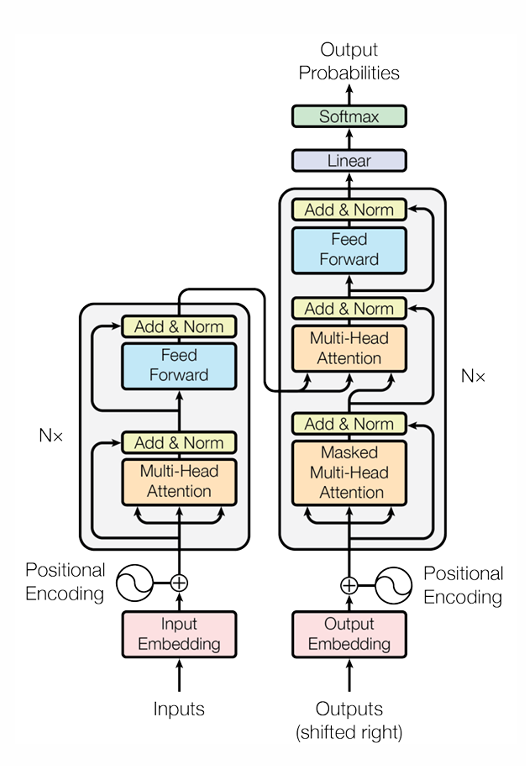
\includegraphics[width=0.4\textwidth]{Immagini/Screenshot 2026-10-25 120911.png} 
\end{figure}

\subsection{Encoder}

L'encoder riceve una sequenza di $T$ token (di solito uno per parola o per istante temporale), ciascuno 
rappresentato da un vettore di dimensione $d_{\text{model}}$. In ingresso e in uscita la forma è la stessa:
\[
\mathbf{X}\in\mathbb{R}^{T\times d_{\text{model}}}
\;\longrightarrow\;
\mathbf{Out}\in\mathbb{R}^{T\times d_{\text{model}}},
\]
senza pooling né riduzione di dimensionalità. Per questo i blocchi si possono impilare: l'uscita di uno è 
l'ingresso del successivo. L'uscita è una sequenza di embedding \emph{contestualizzati}, cioè ogni token è 
la versione dell'ingresso arricchita con l'informazione degli altri token.

Ogni blocco dell'encoder contiene quattro componenti:
\begin{enumerate}
    \item \textbf{Multi-Head Attention (MHA)}: ogni token si confronta con tutti gli altri tramite self-attention.
     È l'unico punto in cui i token si scambiano informazione;
    \item \textbf{Feed Forward}: rete a due livelli lineari con una ReLU in mezzo, applicata separatamente a ciascun token,
    \[
    \operatorname{FFN}(\mathbf{x}) = \max(0,\ \mathbf{x}\mathbf{W}_1+\mathbf{b}_1)\,\mathbf{W}_2+\mathbf{b}_2 ;
    \]
    \item \textbf{Connessione residuale} dopo ciascuno dei due moduli precedenti, che facilita il flusso del gradiente (stessa idea della ResNet);
    \item \textbf{Layer Normalization} dopo ciascuna connessione residuale, per stabilizzare l'addestramento.
\end{enumerate}
\begin{figure}[H]
\centering
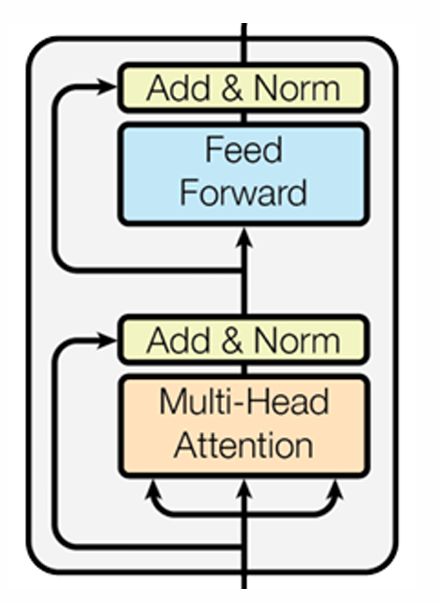
\includegraphics[width=0.4\textwidth]{Immagini/Screenshot 2026-10-25 120926.png} 
\end{figure}

In formule, con $\mathbf{X}$ ingresso del blocco:
\[
\tilde{\mathbf{Z}} = \operatorname{LN}\!\big(\mathbf{X} + \operatorname{MHA}(\mathbf{X})\big),
\qquad
\mathbf{Out} = \operatorname{LN}\!\big(\tilde{\mathbf{Z}} + \operatorname{FFN}(\tilde{\mathbf{Z}})\big).
\]

\paragraph{Dimensioni.} Le proiezioni $\mathbf{Q}$, $\mathbf{K}$, $\mathbf{V}$ hanno dimensione $d_k$, mentre 
l'ingresso ha dimensione $d_{\text{model}}$.
 Con $h$ teste si prende $d_k=d_{\text{model}}/h$, così la concatenazione delle teste ha di nuovo dimensione $d_{\text{model}}$
  e la proiezione finale $\mathbf{W}^O$ riporta all'ingresso la forma richiesta dalla connessione residuale.
  (ES: $d_{\text{model}}=512$, $d_k=64$ e $h=$)

\textbf{OSSERVAZIONE:} nell'encoder la self-attention non ha maschera, quindi ogni token vede tutta la sequenza, 
anche i token successivi. La maschera (causale) serve solo nel decoder, che genera un token alla volta.

\textbf{OSSERVAZIONE:} MHA e FFN hanno ruoli diversi. La MHA mescola l'informazione \emph{tra} i token, 
la FFN trasforma ciascun token \emph{singolarmente}, con gli stessi pesi per tutte le posizioni.

\subsection{Idea dell'attention}

Non tutti gli elementi in ingresso sono ugualmente rilevanti per produrre una data uscita. L'attention
 assegna dinamicamente un peso a ciascun elemento in base alla sua rilevanza nel contesto. 
 Ogni vettore in uscita è una combinazione pesata di \emph{tutti} i vettori in ingresso:
\[
\mathbf{z}_t = \sum_i \alpha_{t,i}\,\mathbf{x}_i, \qquad \alpha_{t,i} = \operatorname{softmax}(s_{t,i}).
\]
I coefficienti $\alpha_{t,i}$ non sono fissi: sono funzioni apprese dell'input.

L'attention funziona come un \textbf{accesso alla memoria per contenuto}: invece di comprimere il contesto 
in un solo stato nascosto (RNN), il modello interroga l'intera sequenza.
\begin{itemize}
    \item \textbf{Key} e \textbf{value}: ogni elemento della sequenza è una cella di memoria, con una chiave 
    (etichetta) e un valore (contenuto);
    \item \textbf{Query}: descrive cosa si sta cercando;
    \item si calcola la similarità tra query e ogni chiave, la softmax la trasforma in pesi, e il risultato è 
    la somma dei valori pesata.
\end{itemize}

\subsection{Query, Key e Value}

Query, key e value si ottengono dall'ingresso $\mathbf{X}\in\mathbb{R}^{T\times d_{\text{model}}}$ (una riga per token) 
con tre proiezioni lineari apprese:
\[
\mathbf{Q} = \mathbf{X}\mathbf{W}^Q, \qquad
\mathbf{K} = \mathbf{X}\mathbf{W}^K, \qquad
\mathbf{V} = \mathbf{X}\mathbf{W}^V,
\]
con $\mathbf{W}^Q,\mathbf{W}^K,\mathbf{W}^V \in \mathbb{R}^{d_{\text{model}}\times d_k}$. Poiché tutte e tre derivano 
dallo stesso $\mathbf{X}$, si parla di \textbf{self-attention}.

\subsection{Scaled dot-product attention}

\[
\operatorname{Attention}(\mathbf{Q},\mathbf{K},\mathbf{V}) = \operatorname{softmax}\!\left(\frac{\mathbf{Q}\mathbf{K}^{\top}}
{\sqrt{d_k}}\right)\mathbf{V}
\]
\begin{enumerate}
    \item $\mathbf{Q}\mathbf{K}^{\top}\in\mathbb{R}^{T\times T}$ è la matrice di similarità: l'elemento $(t,i)$ misura 
    quanto il token $t$ deve guardare il token $i$;
    \item si divide per $\sqrt{d_k}$ ($d_k=64$): con dimensioni grandi i prodotti scalari crescono 
    in modulo e la softmax satura in zone con gradienti piccoli;
    \item la softmax è applicata a ogni riga, quindi i pesi sono in $(0,1)$ e sommano a 1;
    \item si moltiplica per $\mathbf{V}$: ogni token diventa la media pesata dei valori.
\end{enumerate}

\begin{figure}[H]
\centering
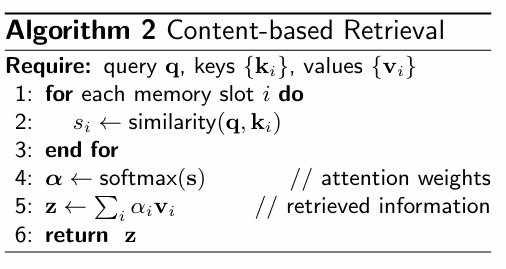
\includegraphics[width=0.4\textwidth]{Immagini/Screenshot 2026-10-25 165420.png} 
\end{figure}

\paragraph{Esempio.} Due token con due feature, e per semplicità $\mathbf{W}^Q=\mathbf{W}^K=\mathbf{W}^V=\mathbf{I}$,
 quindi $\mathbf{Q}=\mathbf{K}=\mathbf{V}=\mathbf{X}$:
\[
\mathbf{X}=\begin{bmatrix}1&0\\1&1\end{bmatrix},\qquad
\mathbf{Q}\mathbf{K}^{\top}=\begin{bmatrix}1&1\\1&2\end{bmatrix},\qquad
\frac{\mathbf{Q}\mathbf{K}^{\top}}{\sqrt{2}}\approx\begin{bmatrix}0.71&0.71\\0.71&1.41\end{bmatrix}
\]
\[
\operatorname{softmax}(\cdot)\approx\begin{bmatrix}0.50&0.50\\0.33&0.67\end{bmatrix},\qquad
\mathbf{Z}\approx\begin{bmatrix}1.00&0.50\\1.00&0.67\end{bmatrix}
\]
Il primo token ha lo stesso prodotto scalare con entrambe le chiavi, quindi pesi uguali. Il secondo è 
più simile a sé stesso (prodotto $2$ contro $1$), quindi dà più peso a sé.

\textbf{Obiettivo: calcolare l'uscita $Z$ per il token ``abbaia''} \\
Contesto in ingresso: [``Il'', ``cane'', ``abbaia'']

\vspace{0.5cm}

\textbf{1. Generazione vettori} (tramite proiezioni $W^Q, W^K, W^V$) \\
Cerco contesto per ``abbaia'': $Q_{\text{abbaia}}$ \\
Etichette disponibili: $K_{\text{Il}}, K_{\text{cane}}, K_{\text{abbaia}}$ \\
Contenuti disponibili: $V_{\text{Il}}, V_{\text{cane}}, V_{\text{abbaia}}$

\vspace{0.5cm}

\textbf{2. Similarità} (Prodotto Scalare $Q K^T$) \\
$S_{\text{Il}} = Q_{\text{abbaia}} \cdot K_{\text{Il}} = 1.2$ \\
$S_{\text{cane}} = Q_{\text{abbaia}} \cdot K_{\text{cane}} = 8.5 \quad \leftarrow \text{(Alta similarità semantica!)}$ \\
$S_{\text{abbaia}} = Q_{\text{abbaia}} \cdot K_{\text{abbaia}} = 3.0$

\vspace{0.5cm}

\textbf{3. Scaling e Softmax} (Pesi $\alpha$)
\[
\alpha = \text{softmax} \left( \frac{[1.2, 8.5, 3.0]}{\sqrt{d_k}} \right) \approx [0.05, 0.85, 0.10]
\]

\textbf{4. Combinazione Pesata Finale} ($\sum \alpha V$)
\[
Z_{\text{abbaia}} = (0.05 \times V_{\text{Il}}) + (0.85 \times V_{\text{cane}}) + (0.10 \times V_{\text{abbaia}})
\]

\subsection{Multi-Head Attention}

Proiezioni e attention sono ripetute in parallelo $h$ volte (es.\ $h=8$), ciascuna con pesi diversi, così ogni testa 
può apprendere un tipo diverso di relazione. Le uscite, ciascuna di dimensione $d_k$, vengono concatenate e proiettate 
con $\mathbf{W}^O$ per tornare a $d_{\text{model}}$:
\[
\operatorname{MHA}(\mathbf{Q},\mathbf{K},\mathbf{V}) = \operatorname{concat}(\mathbf{Z}_1,\dots,\mathbf{Z}_h)\,\mathbf{W}^O,
\qquad
\mathbf{Z}_i = \operatorname{Attention}\!\left(\mathbf{X}\mathbf{W}_i^Q,\ \mathbf{X}\mathbf{W}_i^K,\ \mathbf{X}\mathbf{W}_i^V\right)
\]
Nel paper originale $d_{\text{model}}=512$, $h=8$ e $d_k=d_{\text{model}}/h=64$.

\subsection{Layer Normalization}

La Layer Normalization stabilizza e accelera l'addestramento. Normalizza le attivazioni \emph{sulle feature} 
di ciascun campione, non sul batch:
\[
\operatorname{LN}(\mathbf{x}) = \frac{\mathbf{x}-\mu}{\sigma+\epsilon}\odot\gamma+\beta,
\qquad \mu=\frac{1}{H}\sum_i x_i,
\]
con $\mu$ e $\sigma$ calcolate sulle $H$ feature, e $\gamma,\beta$ parametri appresi.
 Nei Transformer si applica \textbf{per token}.

\textbf{Differenze rispetto alla BatchNorm:}
\begin{itemize}
    \item BatchNorm calcola media e varianza sul batch (per ogni feature); LayerNorm sulle feature di un singolo token;
    \item LayerNorm non dipende dagli altri esempi del batch, né dalla loro lunghezza, e si 
    comporta allo stesso modo in training e in test.
\end{itemize}


\subsection{Dall'encoder alla classificazione}

L'encoder restituisce una sequenza di embedding contestualizzati. Per classificare serve una 
sola rappresentazione. Due strategie:
\begin{itemize}
    \item \textbf{Average pooling}: si calcola $\mathbf{z}_{\text{avg}}=\frac{1}{T}\sum_{t=1}^{T}\mathbf{z}_t$ e lo si passa a un MLP;
    \item \textbf{token [CLS]}: un token speciale viene aggiunto all'inizio della sequenza e il suo
     embedding finale $\mathbf{z}_{[\text{CLS}]}$ è la rappresentazione globale, data in ingresso a un MLP.
\end{itemize}

\subsection{TCN e Transformer a confronto}

Entrambe le architetture servono a modellare dati in sequenza, ma partono da idee diverse.

\begin{center}
\renewcommand{\arraystretch}{1.4}
\begin{tabular}{|p{3.3cm}|p{5.6cm}|p{5.6cm}|}
\hline
 & \textbf{TCN} & \textbf{Transformer} \\
\hline
\textbf{Come lega i dati nel tempo} & convoluzioni causali e dilatate & attention \\
\hline
\textbf{Campo recettivo} & fissato dall'architettura (dimensione del kernel, dilatazione, numero di livelli) 
& non è fissato: il modello impara da solo quali elementi guardare \\
\hline
\textbf{Cosa cattura bene} & struttura locale e di medio raggio & relazioni anche molto lontane nel tempo \\
\hline
\textbf{Addestramento} & stabile e facile da addestrare & --- \\
\hline
\textbf{Tipo di dati} & sequenze ordinate nel tempo & anche contesti multimodali e non sequenziali \\
\hline
\textbf{Modelli noti} & --- & BERT, GPT, ViT \\
\hline
\end{tabular}
\end{center}

\textbf{QUINDI:} le TCN ci impongono in partenza una regola fissa su come guardare il passato; i Transformer imparano
questa regola direttamente dai dati.

\section{Funzioni di costo per la regressione}
\textit{NON LE HANNO SPIEGATE IN AULA, LEGGILE E CHIEDI INFO}

\section{Graph Neural Networks}
\label{sec:gnn}
 
Le Graph Neural Network (GNN) sono reti neurali che lavorano su dati con
struttura a \textbf{grafo}. Le CNN funzionano perché l'immagine è una griglia
regolare; molti dati reali (molecole, reti sociali, reti stradali) non lo sono.
La sezione segue questo ordine:
\begin{enumerate}
  \item perché la convoluzione sulle immagini è già un caso di grafo;
  \item la GCN di Kipf e Welling (message passing);
  \item da dove nasce la sua formula (Laplaciano e convoluzione spettrale);
  \item compiti e applicazioni;
  \item le Graph Attention Network (GAT, GATv2);
  \item GraphCast come esempio reale.
\end{enumerate}
 
%---------------------------------------------------------------------
\subsection{Dalla griglia al grafo}
%---------------------------------------------------------------------
 
\subsubsection{La convoluzione su immagini e su sequenze}
La cross-correlation 2D tra un'immagine $I$ e un kernel quadrato
$K\in\R^{d\times d}$, con $d=2k+1$, è
\[
S(i,j)=\sum_{m=-k}^{k}\sum_{n=-k}^{k} I(i+m,\,j+n)\,K(m,n).
\]
Ad esempio $d=3$ dà $k=1$. È la stessa formula già vista per le CNN, con gli
indici centrati sul pixel. La versione 1D (audio, testo, serie temporali) è
identica con un solo indice: il kernel scorre lungo una retta discretizzata.
 
In entrambi i casi il dominio è un \textbf{reticolo euclideo}: i pixel stanno su
$\mathbb{Z}^2$ (o $\mathbb{Z}$ in 1D), campionamento regolare di un piano
(o di una retta) continuo. Il kernel visita ogni posizione e a ogni passo
tratta una piccola finestra come il \emph{vicinato} del punto.
 
\subsubsection{L'immagine come grafo}
\begin{definizione}[Grafo]
Un grafo $\mathcal{G}=(\mathcal{V},\mathcal{E})$ è formato da un insieme di
nodi $\mathcal{V}$ e da un insieme di archi $\mathcal{E}\subseteq\mathcal{V}\times\mathcal{V}$.
Può essere \textbf{orientato} o non orientato, \textbf{pesato} o non pesato.
Un \textbf{lattice graph} è un grafo con i nodi disposti su una griglia regolare
(1D, 2D o 3D).
\end{definizione}
 
Un'immagine è un segnale su un lattice graph:
\begin{itemize}
  \item ogni pixel è un nodo;
  \item ogni nodo ha un vettore di feature (ad esempio i tre valori RGB);
  \item gli archi collegano ogni nodo ai vicini spaziali con una regola fissa
        (4-connesso: sopra, sotto, sinistra, destra).
\end{itemize}
 
\begin{osservazione}[Conseguenza]
La convoluzione di una CNN è un caso particolare di ``combina un nodo con i suoi
vicini'' su un grafo molto ordinato. Una GNN toglie l'ordine: il grafo può avere
forma qualsiasi.
\end{osservazione}
 
\subsubsection{Limite della convoluzione standard}
Le architetture convoluzionali assumono dati su griglie euclidee, quindi
\textbf{vicinati di forma fissa} e \textbf{invarianza alle traslazioni}.
Molti dati reali sono non euclidei: reti stradali, reti di citazioni tra paper,
grafi molecolari, scheletri del corpo umano (body pose).
 
\subsubsection{Requisiti di una rete su grafi}
\begin{itemize}
  \item \textbf{Struttura irregolare}: i nodi hanno un numero diverso di vicini,
        quindi non esiste un receptive field di dimensione fissa.
  \item \textbf{Nessuna località spaziale}: non c'è una nozione naturale di
        distanza o di ordine tra i nodi.
  \item \textbf{Invarianza alle permutazioni}: l'output non deve dipendere
        dall'ordine in cui i nodi sono elencati o elaborati.
  \item \textbf{Nessun sistema di coordinate globale}: non si può contare su un
        layout o un orientamento fisso.
  \item \textbf{Topologia dinamica}: gli archi possono cambiare nel tempo o
        dipendere dalle feature dei nodi.
\end{itemize}
 
\begin{importante}[Da saper dire a voce]
Un'immagine è un grafo con i pixel come nodi e le adiacenze spaziali come archi.
La convoluzione funziona perché ogni nodo ha sempre lo stesso vicinato. Sui grafi
generici il vicinato ha dimensione e ordine variabili, quindi serve un'operazione
che non dipenda da entrambi: il \emph{message passing}.
\end{importante}
 
%---------------------------------------------------------------------
\subsection{Graph Convolutional Network (GCN)}
%---------------------------------------------------------------------
 
\subsubsection{Idea: message passing}
Le \textbf{Graph Convolutional Network}generalizzano la
convoluzione ai grafi. La struttura è quella di MLP e CNN: layer successivi,
embedding nascosti (qui chiamati \textbf{node embeddings}), funzione di
attivazione, output; i parametri si aggiornano con backpropagation e gradient
descent.
 
L'informazione si propaga lungo il grafo, perché ogni nodo comunica con i vicini.
Un layer fa due passi:
\begin{enumerate}
  \item \textbf{Aggregazione}: ogni nodo combina gli embedding dei vicini con una
        funzione di aggregazione (somma, media, massimo o una funzione appresa) che 
        non dipendono dall'ordine degli addendi(\textit{l'invarianza alle permutazioni}).
  \item \textbf{Aggiornamento}: il risultato passa in una rete neurale (ad
        esempio un MLP) che produce il nuovo embedding del nodo. L'embedding
        nuovo contiene le feature del nodo e quelle del suo vicinato.
\end{enumerate}
 
\begin{center}
\begin{tikzpicture}[nd/.style={circle,draw,minimum size=0.85cm,inner sep=0pt}]
\node[nd,fill=fmapcol] (v) at (0,0) {$v$};
\node[nd] (a) at (-2.2,1.0) {$u_1$};
\node[nd] (b) at (2.2,1.0) {$u_2$};
\node[nd] (c) at (0,-1.9) {$u_3$};
\draw[-{Stealth},thick] (a)--(v);
\draw[-{Stealth},thick] (b)--(v);
\draw[-{Stealth},thick] (c)--(v);
\draw[-{Stealth},thick,dashed] (v) to[out=60,in=120,looseness=9] (v);
\node[font=\small,anchor=west] at (2.9,-0.3) {$\mathbf{a}_v=\text{aggrega}\big(\{\mathbf{h}_u\}\big)$};
\node[font=\small,anchor=west] at (2.9,-0.95) {$\mathbf{h}_v'=\text{MLP}(\mathbf{a}_v)$};
\end{tikzpicture}
\captionof{figure}{Message passing: $v$ riceve i messaggi dai vicini e da sé stesso (self-loop tratteggiato)}
\end{center}

\begin{figure}[H]
\centering
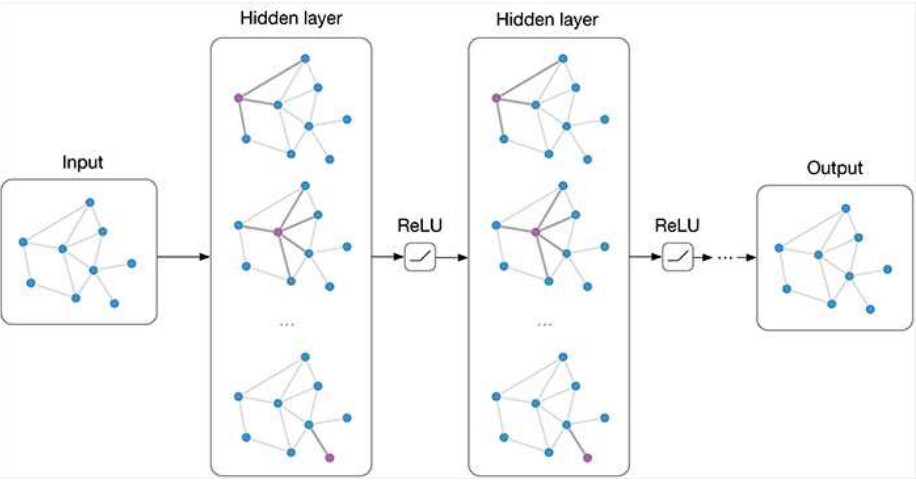
\includegraphics[width=0.4\textwidth]{Immagini/Screenshot 2026-11-09 180443.png} 
\end{figure}


 
\subsubsection{Input della GCN}
\begin{itemize}
  \item \textbf{Matrice delle feature} $X\in\R^{n\times d}$: una riga per nodo.
  \item \textbf{Matrice di adiacenza} $A\in\R^{n\times n}$: codifica la struttura
        del grafo (binaria o pesata).
\end{itemize}

\begin{figure}[H]
\centering
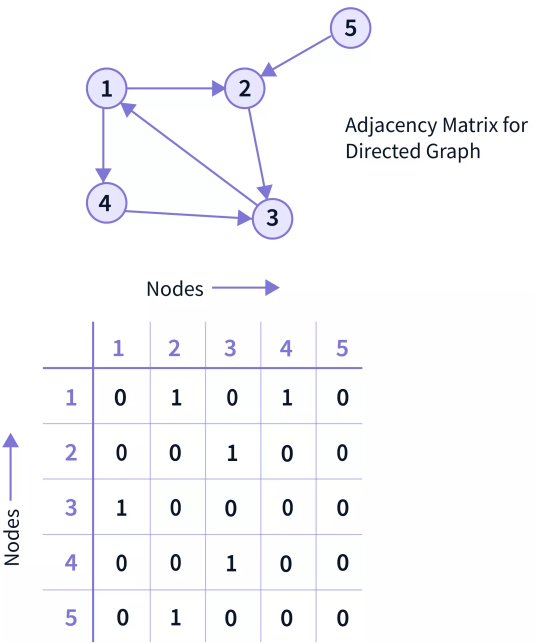
\includegraphics[width=0.4\textwidth]{Immagini/Screenshot 2026-11-09 180708.png} 
\end{figure}
 
\textbf{Ruolo di $A$.} È un \textbf{prior strutturale} sulla geometria del
dominio: dice quali nodi possono scambiarsi messaggi. Questo
\begin{itemize}
  \item impone località e limita il message passing alle connessioni sensate;
  \item inietta un bias induttivo nel modello;
  \item riduce l'overfitting e aiuta la generalizzazione.
\end{itemize}
\textbf{Da dove viene $A$:}
\begin{itemize}
  \item conoscenza del dominio(impostati manualmente) (giunti di uno scheletro, legami
        chimici);
  \item costruzione euristica: $k$-nearest neighbors nello spazio delle feature,
        soglie sulla distanza.
\end{itemize}
 
\subsubsection{Regola di propagazione}
\begin{definizione}[Layer GCN]
\[
\mathbf{H}^{(\ell)}=\sigma\!\left(\hat{\mathbf{D}}^{-1/2}\,\hat{\mathbf{A}}\,\hat{\mathbf{D}}^{-1/2}\,\mathbf{H}^{(\ell-1)}\,\mathbf{W}^{(\ell)}\right)
\]
\begin{itemize}
  \item $\hat{\mathbf{A}}=\mathbf{A}+\mathbf{I}$: adiacenza con self-loop;
  \item $\hat{\mathbf{D}}$: matrice diagonale dei gradi, $\hat{\mathbf{D}}_{ii}=\sum_j\hat{\mathbf{A}}_{ij}$ (Numero di archi connessi al nodo);
  \item $\hat{\mathbf{D}}^{-1/2}\hat{\mathbf{A}}\hat{\mathbf{D}}^{-1/2}$: normalizzazione simmetrica
        dell'adiacenza, indicata nel seguito con $\hat{S}$;
  \item $\mathbf{H}^{(\ell-1)}\in\R^{|\mathcal{V}|\times F_{\ell-1}}$: embedding del layer precedente
        (con $\mathbf{H}^{(0)}=X$);
  \item $\mathbf{W}^{(\ell)}\in\R^{F_{\ell-1}\times F_\ell}$: matrice di proiezione appresa;
  \item $\sigma$: non-linearità (ad esempio ReLU).
\end{itemize}
\end{definizione}
 
I due fattori hanno compiti separati: $\hat{S}$ mescola i \textbf{nodi}
(ogni riga è una media pesata dei vicini e del nodo stesso), $\mathbf{W}$ mescola
le \textbf{feature} (cambia la dimensione da $F_{\ell-1}$ a $F_\ell$).
 
\textbf{Forma per singolo nodo} (valida per adiacenza binaria):
\[
\mathbf{a}_v^{(\ell)}=\sum_{u\in\mathcal{N}(v)\cup\{v\}}\frac{1}{\sqrt{\hat d_v\hat d_u}}\,\mathbf{h}_u^{(\ell-1)},
\qquad
\mathbf{z}_v^{(\ell)}=\mathbf{a}_v^{(\ell)}\mathbf{W}^{(\ell)},
\qquad
\mathbf{h}_v^{(\ell)}=\sigma\big(\mathbf{z}_v^{(\ell)}\big).
\]
Sono i tre passi \emph{aggregazione, proiezione, non-linearità}. $\hat d_v$ è il
grado di $v$ contando il self-loop.
 
\textbf{Perché il self-loop.} Senza di esso $\mathbf{h}_v$ dipenderebbe solo dai
vicini e il nodo perderebbe le proprie feature.
 
\textbf{Perché la normalizzazione.} Con una somma semplice un nodo con molti
vicini produrrebbe valori molto più grandi di uno con pochi. Il fattore
$1/\sqrt{\hat d_v\hat d_u}$ pesa meno i collegamenti con nodi di grado alto e
tiene le scale confrontabili.
 
\begin{osservazione}[Esempio numerico]
Grafo a catena $1-2-3$ con una sola feature per nodo, $x=(1,2,3)^\top$.
\[
\hat{A}=\begin{bmatrix}1&1&0\\1&1&1\\0&1&1\end{bmatrix},\quad
\hat{D}=\operatorname{diag}(2,3,2),\quad
\hat{S}=\begin{bmatrix}\tfrac12&\tfrac1{\sqrt6}&0\\[2pt]\tfrac1{\sqrt6}&\tfrac13&\tfrac1{\sqrt6}\\[2pt]0&\tfrac1{\sqrt6}&\tfrac12\end{bmatrix}
\]
Per il nodo 1: $\tfrac12\cdot1+\tfrac1{\sqrt6}\cdot2\approx1.32$.
Per il nodo 2: $\tfrac1{\sqrt6}\cdot1+\tfrac13\cdot2+\tfrac1{\sqrt6}\cdot3\approx2.30$.
Per il nodo 3: $\tfrac1{\sqrt6}\cdot2+\tfrac12\cdot3\approx2.32$.
Quindi $\hat{S}x\approx(1.32,\ 2.30,\ 2.32)^\top$: i valori si avvicinano tra loro.
Poi si moltiplica per $\mathbf{W}$ e si applica $\sigma$.
\end{osservazione}
 
\subsubsection{Receptive field e GCN a due layer}
Un layer aggrega i vicini a \textbf{1 hop} (primo ordine). Impilando $L$ layer
un nodo riceve informazione dai nodi a distanza al più $L$. Per la
classificazione dei nodi con due layer:
\[
\mathbf{Z}=\operatorname{softmax}\!\Big(\hat{S}\;\sigma\big(\hat{S}\,X\,\mathbf{W}^{(0)}\big)\;\mathbf{W}^{(1)}\Big).
\]
 
\begin{importante}[Da saper dire a voce]
Un layer GCN fa una media pesata sul vicinato (con self-loop) e poi una
trasformazione lineare appresa. La matrice $\hat{S}$ dipende solo dal grafo e
dice \emph{chi parla con chi}; $\mathbf{W}$ è appresa e dice \emph{come combinare le
feature}. Con $L$ layer si raggiungono i vicini a $L$ hop.
\end{importante}
 
%---------------------------------------------------------------------
\subsection{Motivazione teorica: convoluzione spettrale e Laplaciano}
%---------------------------------------------------------------------
 
La GCN si può derivare con la teoria spettrale sui grafi: è un'\textbf{approssimazione
al primo ordine delle convoluzioni spettrali su grafo}'
Il percorso ha cinque passaggi.
 
\subsubsection{1. Il Laplaciano è un filtro}
Grafo non orientato e non pesato con $N$ nodi e adiacenza $A$. Sia
$d_i=\sum_jA_{ij}>0$, $D=\operatorname{diag}(d_1,\dots,d_N)$ e $x\in\R^N$ un
segnale con un valore per nodo. Si definiscono
\[
S=D^{-1/2}AD^{-1/2},\qquad L=I-S\quad\text{(Laplaciano normalizzato)}.
\]
Applicato a un segnale,
\[
(Lx)_i=x_i-\sum_{j:\,A_{ij}=1}\frac{x_j}{\sqrt{d_id_j}},
\]
cioè ``il valore del nodo meno la media pesata dei vicini'': il Laplaciano
combina già un nodo con il suo vicinato.
 
Un \textbf{autovettore} $u$ soddisfa $Lu=\lambda u$ e $\lambda$ è il suo
\textbf{autovalore}. Allora $L^ku=\lambda^ku$ e, per un polinomio
$p(L)=a_0I+a_1L+\dots+a_KL^K$,
\[
p(L)\,u=\underbrace{(a_0+a_1\lambda+\dots+a_K\lambda^K)}_{p(\lambda)}\,u .
\]
 
\begin{importante}[Risultato chiave]
Un polinomio in $L$ scala ogni autovettore separatamente. Un \textbf{filtro
spettrale} è un moltiplicatore $g(\lambda)$ per ogni autovalore. Se $g=p$ è un
polinomio, il filtraggio è esattamente $y=p(L)x$. Il semplice prodotto $Lx$ è il
caso $g(\lambda)=\lambda$.
\end{importante}
 
\subsubsection{2. Trasformata di Fourier su grafo e convoluzione spettrale}
$L$ è simmetrica, quindi si possono scegliere autovettori $u_1,\dots,u_N$ di
lunghezza uno e a due a due perpendicolari. Raccolti in colonne:
\[
U=[u_1\ \cdots\ u_N],\quad \Lambda=\operatorname{diag}(\lambda_1,\dots,\lambda_N),\quad
U^\top U=UU^\top=I,\quad L=U\Lambda U^\top .
\]
Ogni segnale ha l'espansione
\[
x=\sum_{r=1}^{N}\hat x_r\,u_r,\qquad \hat x_r=u_r^\top x,\qquad \hat x=U^\top x .
\]
Il vettore $\hat x$ è la \textbf{graph Fourier transform}: le coordinate di $x$
nella base degli autovettori.
 
\begin{definizione}[Convoluzione spettrale su grafo]
\[
y=\sum_{r=1}^{N}g(\lambda_r)\,\hat x_r\,u_r=U\,g(\Lambda)\,U^\top x,
\qquad g(\Lambda)=\operatorname{diag}\big(g(\lambda_1),\dots,g(\lambda_N)\big).
\]
\emph{Lettura:} $U^\top$ cambia coordinate, $g(\Lambda)$ scala ogni componente,
$U$ ricostruisce il segnale.
\end{definizione}
 
\textbf{Problema.} Calcolare e memorizzare tutti gli autovettori è costoso sui
grafi grandi (Kipf e Welling, Sez.~2.1).
 
\begin{osservazione}[Perché si parla di frequenze (non nelle slide)]
Gli autovalori di $L$ stanno in $[0,2]$. Gli autovettori con $\lambda$ piccolo
cambiano poco tra nodi collegati (``basse frequenze''); quelli con $\lambda$
grande oscillano tra nodi vicini (``alte frequenze''). Per $S=I-L$ l'autovalore
corrispondente è $1-\lambda$, per $I+S$ è $2-\lambda$: entrambi \emph{decrescono}
con $\lambda$. Applicare $I+S$ o $\hat{S}$ mantiene le basse frequenze e smorza le
alte, cioè \textbf{lisci}a il segnale. È la stessa idea dell'esempio numerico
sopra, e spiega l'over-smoothing quando i layer sono molti.
\end{osservazione}
 
\subsubsection{3. Polinomi di Chebyshev: costruire il filtro}
Invece di imparare una $g(\lambda)$ qualsiasi, la si approssima con un polinomio
di grado $K$ scritto nella base di Chebyshev:
\[
T_0(z)=1,\qquad T_1(z)=z,\qquad T_k(z)=2z\,T_{k-1}(z)-T_{k-2}(z)\quad(k\ge2).
\]
I $T_k$ restano in $[-1,1]$ quando $z\in[-1,1]$ e si calcolano per ricorrenza.
Gli autovalori si riscalano in quell'intervallo con $\lambda_{\max}$ il più
grande:
\[
\widetilde\lambda=\frac{2\lambda}{\lambda_{\max}}-1,\qquad
0\mapsto-1,\quad\lambda_{\max}\mapsto1,\qquad
\widetilde\Lambda=\frac{2\Lambda}{\lambda_{\max}}-I .
\]
Il filtro di grado $K$ ha $K+1$ coefficienti appresi:
\[
g(\lambda)\approx\sum_{k=0}^{K}c_k\,T_k(\widetilde\lambda)
\quad\Longrightarrow\quad
g(\Lambda)\approx\sum_{k=0}^{K}c_k\,T_k(\widetilde\Lambda).
\]
Si imparano direttamente $c_0,\dots,c_K$ (Defferrard et al., 2016, Sez.~2.1).
Un $K$ piccolo restringe le forme di filtro disponibili.
 
\subsubsection{4. Eliminare $U$: un'identità esatta}
Sia $\widetilde L=2L/\lambda_{\max}-I=U\widetilde\Lambda U^\top$. Poiché $U^\top U=I$,
\[
\widetilde L^{\,2}=U\widetilde\Lambda\underbrace{U^\top U}_{I}\widetilde\Lambda U^\top=U\widetilde\Lambda^{2}U^\top .
\]
La stessa cancellazione vale per ogni potenza, quindi per ogni polinomio:
\[
U\,T_k(\widetilde\Lambda)\,U^\top=T_k(\widetilde L),\qquad T_0(\widetilde L)=I,\quad T_2(\widetilde L)=2\widetilde L^{\,2}-I .
\]
Allora
\[
y=Ug(\Lambda)U^\top x\;\approx\;\sum_{k=0}^{K}c_k\,U\,T_k(\widetilde\Lambda)\,U^\top x\;=\;\sum_{k=0}^{K}c_k\,T_k(\widetilde L)\,x .
\]
\textbf{Solo la scelta di un filtro polinomiale è un'approssimazione; l'ultima
uguaglianza è esatta.} Si calcola per ricorrenza, senza autovettori:
\[
v_0=x,\qquad v_1=\widetilde L\,x,\qquad v_k=2\widetilde L\,v_{k-1}-v_{k-2},
\qquad y\approx\sum_{k=0}^{K}c_k v_k .
\]
Servono solo prodotti matrice-vettore con $\widetilde L$ (matrice sparsa).
 
\subsubsection{5. Le semplificazioni di Kipf e Welling}
\textbf{(a) Grado uno e $\lambda_{\max}\approx2$.} Per il Laplaciano normalizzato
$\lambda_{\max}\le2$. Con $\lambda_{\max}=2$ si ha $\widetilde L\approx L-I=-S$ e
\[
y\approx c_0\,x-c_1\,Sx\;\xrightarrow{\;c_0=\theta,\ c_1=-\theta\;}\;\theta\,(I+S)\,x .
\]
Imporre $c_0=-c_1=\theta$ è una scelta di modellazione aggiuntiva: riduce i
parametri a uno solo.
 
\textbf{(b) Self-loop e rinormalizzazione.} Si definiscono
\[
\hat{A}=A+I,\qquad \hat{D}_{ii}=d_i+1,\qquad \hat{S}=\hat{D}^{-1/2}\hat{A}\hat{D}^{-1/2},
\]
e si sostituisce $I+S$ con $\hat{S}$. Questo è un \textbf{cambio di operatore},
\emph{non} un'uguaglianza algebrica. Il vantaggio: $I+S$ ha autovalori in
$[0,2]$ e applicato più volte può amplificare i segnali; $\hat{S}$ ha autovalori
di modulo al più $1$ e limita l'amplificazione nella propagazione.
 
\textbf{(c) Più feature per nodo.} Con $F_\ell$ feature per nodo, $\mathbf{H}^{(\ell)}\in\R^{N\times F_\ell}$,
e una matrice $\mathbf{W}^{(\ell)}\in\R^{F_\ell\times F_{\ell+1}}$ che combina le
feature:
\begin{center}
\fbox{\(\displaystyle \mathbf{H}^{(\ell+1)}=\sigma\!\big(\hat{S}\,\mathbf{H}^{(\ell)}\,\mathbf{W}^{(\ell)}\big)\)}
\end{center}
Che è la regola di propagazione della sezione precedente.
 
\begin{center}
\renewcommand{\arraystretch}{1.35}
\begin{tabular}{|p{3.6cm}|p{10.6cm}|}
\hline
\textbf{Passaggio} & \textbf{Cosa succede} \\
\hline
Laplaciano $L=I-S$ & misura la differenza tra un nodo e i vicini; un polinomio di $L$ è un filtro \\
\hline
Convoluzione spettrale & $y=Ug(\Lambda)U^\top x$; richiede gli autovettori, costosi \\
\hline
Chebyshev & il filtro è un polinomio di grado $K$ con $K+1$ coefficienti da imparare \\
\hline
Eliminare $U$ & $UT_k(\widetilde\Lambda)U^\top=T_k(\widetilde L)$: niente più autovettori \\
\hline
Kipf e Welling & $K=1$, $\lambda_{\max}\approx2$, un solo parametro, self-loop e rinormalizzazione: $\hat{S}$ \\
\hline
Layer finale & $\mathbf{H}^{(\ell+1)}=\sigma(\hat{S}\mathbf{H}^{(\ell)}\mathbf{W}^{(\ell)})$ \\
\hline
\end{tabular}
\end{center}
 
\begin{importante}[Da saper dire a voce]
La convoluzione ideale su grafo è $U g(\Lambda) U^\top x$, ma richiede gli
autovettori del Laplaciano. Approssimando $g$ con un polinomio di Chebyshev gli
autovettori spariscono (un polinomio di $\widetilde\Lambda$ si trasforma in un
polinomio di $\widetilde L$). Kipf e Welling prendono il grado uno, un solo
parametro e $\lambda_{\max}\approx2$, poi aggiungono self-loop e rinormalizzano
per stabilità: ne esce $\hat{S}$, che è la media pesata sul vicinato.
\end{importante}
 

%---------------------------------------------------------------------
\subsection{Compiti e applicazioni}


Le GNN possono essere utilizzate per diversi compiti, a seconda di
che cosa vogliamo prevedere:

\begin{itemize}
    \item \textbf{Node classification}: classificare i singoli nodi.
    \item \textbf{Link prediction}: prevedere le connessioni tra nodi.
    \item \textbf{Graph classification}: classificare un intero grafo.
    \item \textbf{Community detection}: individuare gruppi di nodi
    fortemente connessi.
    \item \textbf{Anomaly detection}: individuare nodi o connessioni
    anomale.
\end{itemize}

\begin{figure}[H]
\centering
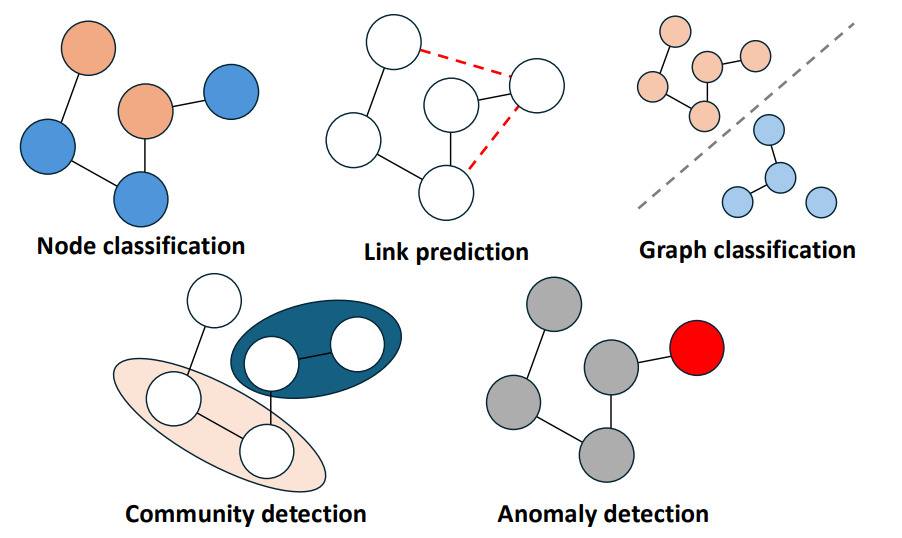
\includegraphics[width=0.4\textwidth]{Immagini/Screenshot 2026-11-09 183541.png} 
\end{figure}

\subsubsection{Node classification}

Obiettivo: assegnare una classe a ciascun nodo del grafo.

La GNN raccoglie le feature del nodo e dei suoi vicini, producendo
un embedding $\mathbf{h}_v$. Un classificatore utilizza questo
vettore per prevedere la classe:

\[
\mathbf{z}_v = W\mathbf{h}_v+b,
\qquad
\hat y_v=\arg\max_c \mathbf{z}_v[c]
\]

Applicazioni:
\begin{itemize}
    \item Reti sociali: classificare gli utenti.
    \item Reti di citazioni: prevedere l'argomento di un paper.
    \item Molecole: riconoscere il tipo di atomo.
\end{itemize}

\textbf{Setting trasduttivo e induttivo}

\begin{itemize}
    \item \textbf{Trasduttivo}: durante il training è disponibile
    l'intero grafo, ma solo alcuni nodi hanno un'etichetta.
    Il modello deve classificare i nodi rimanenti dello stesso grafo.

    \item \textbf{Induttivo}: il modello deve classificare nodi
    o grafi mai incontrati durante il training, generalizzando
    a nuove strutture.
\end{itemize}

\begin{figure}[H]
\centering
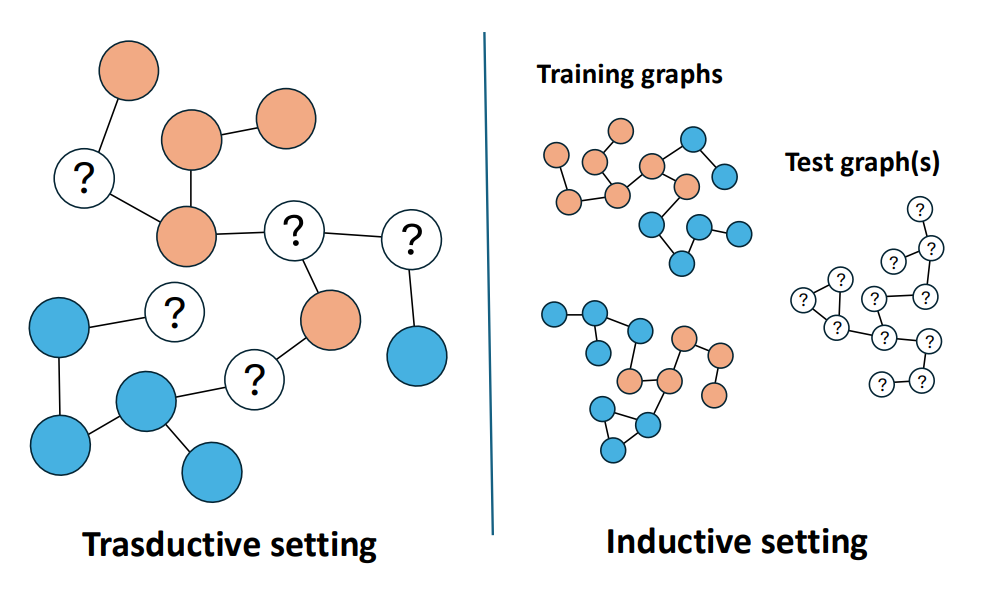
\includegraphics[width=0.4\textwidth]{Immagini/Screenshot 2026-11-09 191220.png} 
\end{figure}

\subsubsection{Link prediction}

Obiettivo: prevedere se due nodi sono collegati da un arco.

La GNN produce gli embedding dei due nodi, che vengono utilizzati
da un decoder per calcolare un punteggio di compatibilità:

\[
s_{uv}=\operatorname{Decoder}(\mathbf{h}_u,\mathbf{h}_v)
\]

Un classificatore utilizza il risultato per stabilire se
la connessione esiste.

Applicazioni:
\begin{itemize}
    \item Raccomandazioni: prevedere se un utente apprezzerà
    un prodotto.
    \item Reti sociali: prevedere nuove amicizie.
    \item Biologia: prevedere interazioni tra proteine.
\end{itemize}

\subsubsection{Graph classification}

Obiettivo: assegnare una classe a un intero grafo,
anziché ai singoli nodi.

La GNN produce un embedding per ogni nodo. Una funzione di
\textbf{global pooling} li combina in un unico vettore,
che rappresenta l'intero grafo.

\[
\mathbf{h}_{graph}
=
\operatorname{POOLING}
\left(\{\mathbf{h}_v\mid v\in\mathcal{V}\}\right)
\]

Un MLP utilizza questo vettore per classificare il grafo.

Principali tecniche di pooling:

\begin{itemize}
    \item \textbf{Average pooling}: calcola la media degli
    embedding dei nodi.
    \[
    \mathbf{h}_{graph}
    =\frac{1}{|\mathcal{V}|}
    \sum_{v\in\mathcal{V}}\mathbf{h}_v
    \]

    \item \textbf{Attention pooling}: assegna pesi diversi
    ai nodi, dando maggiore importanza a quelli più rilevanti.
    \[
    \mathbf{h}_{graph}
    =\sum_v\alpha_v\mathbf{h}_v
    \]
\end{itemize}

Esiste anche il \textbf{pooling gerarchico} (es. DiffPool),
che riduce progressivamente il grafo, in modo simile al
pooling delle CNN.

\begin{figure}[H]
\centering
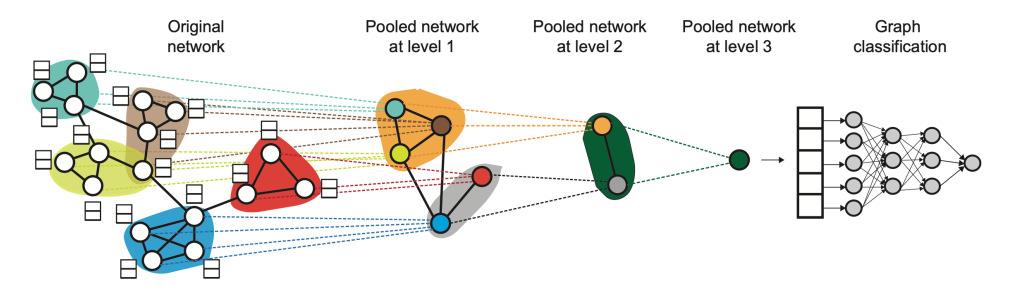
\includegraphics[width=0.6\textwidth]{Immagini/Screenshot 2026-11-09 191609.png} 
\end{figure}

\textbf{Esempio: riconoscimento delle azioni umane.}

Una sequenza di pose umane viene rappresentata attraverso
un grafo:
\begin{itemize}
    \item Nodi: articolazioni del corpo.
    \item Archi spaziali: collegamenti tra articolazioni.
    \item Archi temporali: collegamenti della stessa articolazione
    tra frame consecutivi.
\end{itemize}

\begin{figure}[H]
\centering
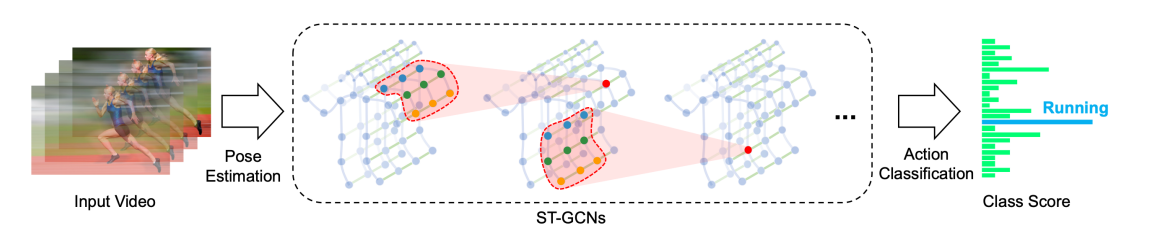
\includegraphics[width=0.8\textwidth]{Immagini/Screenshot 2026-11-09 191753.png} 
\end{figure}

Una GNN spazio-temporale (ST-GCN) analizza le relazioni
tra articolazioni e la loro evoluzione nel tempo per
riconoscere l'azione eseguita.


%---------------------------------------------------------------------
\subsection{Graph Attention Network (GAT)}
%---------------------------------------------------------------------

\subsubsection{Limiti della GCN}

La GCN aggrega le informazioni dei nodi vicini utilizzando
pesi determinati dalla struttura e dalla normalizzazione
del grafo. Presenta però alcuni limiti:

\begin{itemize}
    \item \textbf{Over-smoothing}: al crescere dei layer le rappresentazioni dei nodi diventano 
    indistinguibili.
    \item \textbf{Pesi non adattivi}: i vicini contribuiscono con lo stesso peso,
     a meno della normalizzazione per grado, senza attention nè pesi adattivi.
    \item \textbf{Dipendenza dall'adiacenza}: GCN dipende fortemente dalle relazioni codi cate 
    nella matrice di adiacenza in ingresso.
\end{itemize}

\subsubsection{Idea della GAT}
Le \textbf{Graph Attention Network}  usano un meccanismo
di attention: ogni nodo ``guarda'' i vicini e assegna a ciascuno un peso
\emph{appreso}.
\begin{itemize}
  \item \textbf{Pesi sugli archi appresi}: non serve una matrice di adiacenza
        pesata definita a priori.
  \item \textbf{Adattività locale}: vicini diversi ricevono pesi diversi.
\end{itemize}
L'adiacenza serve solo a dire quali coppie possono attendersi.

\begin{figure}[H]
\centering
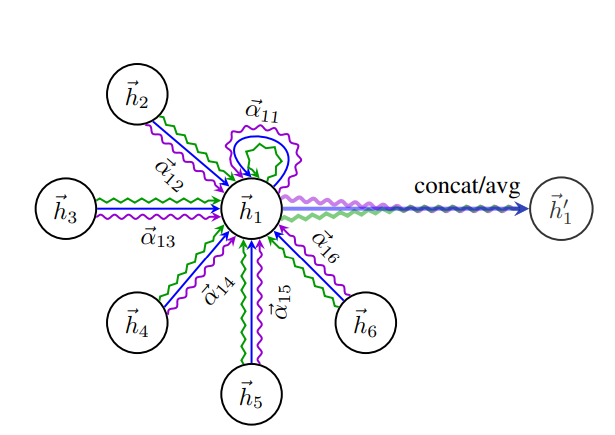
\includegraphics[width=0.6\textwidth]{Immagini/Screenshot 2026-11-09 192335.png} 
\end{figure}

\subsubsection{Funzionamento della GAT}

Il calcolo avviene in quattro passaggi principali.

\textbf{1. Proiezione lineare}

Le feature di ogni nodo vengono trasformate attraverso
una matrice di pesi condivisa($W$ appresa):

\[
\mathbf{h}_i^W=\mathbf{W}\mathbf{h}_i
\]

\textbf{2. Calcolo dell'attention}

Per ogni nodo $i$ e ogni suo vicino $j$ si calcola
un punteggio di affinità.($a$ appreso):

\[
e_{ij}=
\operatorname{LeakyReLU}
\left(
\mathbf{a}^{\top}
[\mathbf{h}_i^W\Vert\mathbf{h}_j^W]
\right)
\]

Dove $e_{ij}$ misura quanto le informazioni di $j$
sono importanti per $i$. (dim = SCALARE)

\begin{osservazione}
  \textit{QUANTE OPERAZIONI DEVO FARE COME STEP 1,2 ?} $\rightarrow \binom{N}{2}$
\end{osservazione}

\textbf{Matrice dei coefficienti non normalizzati ($e_{ij}$):}\\
  Applicazione della \texttt{softmax} riga per riga per i nodi $V_1, V_2, V_3$ 
  (dove ogni riga ha \textit{somma = 1}):
  \begin{equation*}
      \begin{bmatrix}
          e_{1,1} & e_{1,2} & -\infty \\
          e_{2,1} & e_{2,2} & e_{2,3} \\
          -\infty & e_{3,2} & e_{3,3}
      \end{bmatrix}
  \end{equation*}
I valori $-\infty$ rappresentano l'assenza di un arco e \textbf{è ZERO DOPO SOFTMAX}.

\textbf{Passo 3.} Calcolo dei punteggi di attenzione normalizzati su tutti i vicini di $i$:
\begin{equation}
    \alpha_{ij} = \frac{\exp(e_{ij})}{\sum_{k \in \mathcal{N}(i)} \exp(e_{ik})}
\end{equation}

\begin{figure}[H]
\centering
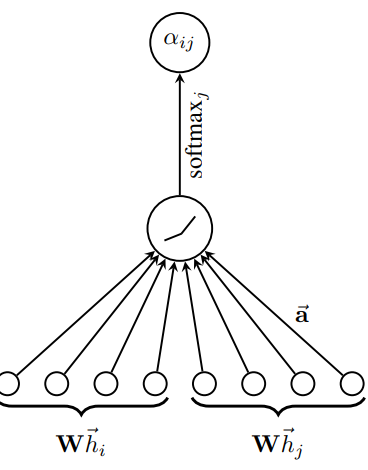
\includegraphics[width=0.2\textwidth]{Immagini/Screenshot 2026-11-09 194607.png} 
\end{figure}

\textbf{Passo 4.} Calcolo dell'embedding finale come somma pesata:
\begin{equation}
    \mathbf{h}_i' = \sigma \left( \sum_{j \in \mathcal{N}(i)} \alpha_{ij} \mathbf{h}_j \mathbf{W} \right)
\end{equation}

\textit{USA LA MATRICE FINALE PER ASSEGNARE IL NUOVO VALORE.}\\
    \textbf{Spiegazione dello Step 4:} La matrice finale $\alpha$ contiene le percentuali di importanza.
     Si prendono le feature dei vicini trasformate ($\mathbf{h}_j \mathbf{W}$), 
     le si moltiplicano per le rispettive percentuali ($\alpha_{ij}$), 
     si somma tutto e si applica un'ultima non-linearità ($\sigma$). 
     Questo genera il nuovo embedding $\mathbf{h}_i'$ in cui il nodo ha filtrato attivamente le 
     informazioni ricevute.

\begin{osservazione}
    \textit{Perché serve la LeakyReLU prima della Softmax?} 
    \begin{enumerate}
        \item \textbf{Perdita di espressività:} Se si usa solo una proiezione lineare seguita da Softmax
         (saltando la LeakyReLU), si toglie una non-linearità fondamentale per l'apprendimento.
        \item \textbf{Impossibilità di ignorare il rumore:} La LeakyReLU permette 
        di mandare in negativo gli score dei vicini inutili. Senza di essa, 
        la Softmax non riuscirebbe a schiacciare a zero i coefficienti $\alpha$ dei vicini irrilevanti. 
        L'attenzione rimarrebbe troppo "piatta" e il nodo faticherebbe a spegnere i collegamenti inutili.
    \end{enumerate}
\end{osservazione}

\textit{ RIVEDI:
L'attention viene calcolata soltanto sui vicini indicati
dalla matrice di adiacenza, incluso il nodo stesso.
In questo modo si mantiene la struttura del grafo
e non è necessario confrontare tutte le coppie di nodi.}

\subsubsection{Multi-head attention}

È possibile utilizzare $K$ meccanismi di attention
indipendenti, chiamati \textbf{head}.

Ogni head calcola una propria aggregazione; i risultati
vengono poi concatenati:

\[
\mathbf{h}'_i=
\big\Vert_{k=1}^{K}
\sigma\left(
\sum_{j\in\mathcal{N}(i)}
\alpha_{ij}^{(k)}
\mathbf{W}^{(k)}\mathbf{h}_j
\right)
\]

La concatenazione produce un embedding con $KF'$ feature.
Nell'ultimo layer si può utilizzare anche la media
delle head anziché la concatenazione.

\subsubsection{GAT e Self-Attention}

Entrambe utilizzano l'attention, ma differiscono
per il modo in cui vengono selezionate le informazioni.

\begin{center}
\renewcommand{\arraystretch}{1.35}
\begin{tabular}{|p{3.2cm}|p{5.9cm}|p{5.9cm}|}
\hline
\textbf{Aspetto} & \textbf{GAT} & \textbf{Self-attention (Transformer)} \\
\hline
Input & grafo (nodi e archi) & sequenza (ad esempio token) \\
\hline
Vicinato & definito dalla matrice di adiacenza & ogni token attende tutti gli altri \\
\hline
Sparsità & sparsa: solo i vicini locali & densa: interazioni a coppie complete \\
\hline
Meccanismo & MLP a un livello sulle coppie concatenate & prodotto scalare tra query e key apprese \\
\hline
Posizione & implicita nella topologia del grafo & esplicita (sinusoidale o appresa) \\
\hline
Bias induttivo & locale e relazionale, dagli archi & temporale o spaziale, dalle codifiche posizionali \\
\hline
\end{tabular}
\end{center}

La differenza principale è che la GAT sfrutta la struttura
del grafo e calcola l'attention solo tra nodi collegati,
mentre il Transformer standard considera tutte le coppie
di token.

\subsubsection{GATv2}

La GAT standard presenta un limite: utilizza una
\textbf{attention statica}.

In particolare, l'ordinamento dei vicini in base
all'importanza non dipende dal nodo che sta effettuando
l'attenzione. Di conseguenza, nodi diversi non possono
modificare dinamicamente la priorità assegnata agli stessi
vicini.

La GATv2 risolve questo problema
modificando l'ordine delle operazioni.

\[
\begin{aligned}
\text{GAT:}\quad
&e_{ij}=
\operatorname{LeakyReLU}
\left(
\mathbf{a}^{\top}
[\mathbf{W}\mathbf{h}_i\Vert\mathbf{W}\mathbf{h}_j]
\right)
\\[6pt]
\text{GATv2:}\quad
&e_{ij}=
\mathbf{a}^{\top}
\operatorname{LeakyReLU}
\left(
\mathbf{W}
[\mathbf{h}_i\Vert\mathbf{h}_j]
\right)
\end{aligned}
\]

La non-linearità viene applicata prima del vettore
$\mathbf{a}$, rendendo il punteggio dipendente
dinamicamente dalla coppia di nodi.

\textbf{Differenza da ricordare:}
\begin{itemize}
    \item GAT: attention statica.
    \item GATv2: attention dinamica, più espressiva.
\end{itemize}


\begin{importante}[Da ricordare]
La GAT migliora la GCN introducendo pesi di attention
appresi sui vicini. La GATv2 modifica il calcolo di questi
pesi per ottenere un meccanismo di attention dinamica.
\end{importante}

%---------------------------------------------------------------------
\subsection{GraphCast}
%---------------------------------------------------------------------

% \textbf{GraphCast} è un modello basato
% su GNN utilizzato per prevedere il tempo atmosferico
% a medio termine.

% L'idea è rappresentare l'atmosfera come un grafo:

% \begin{itemize}
%     \item \textbf{Nodi}: punti distribuiti su una mesh
%     sferica (icosaedrica).
%     \item \textbf{Archi}: collegamenti tra punti
%     geograficamente vicini.
%     \item \textbf{Feature}: variabili meteorologiche,
%     come temperatura, pressione e vento.
% \end{itemize}

% \begin{figure}[H]
% \centering
% 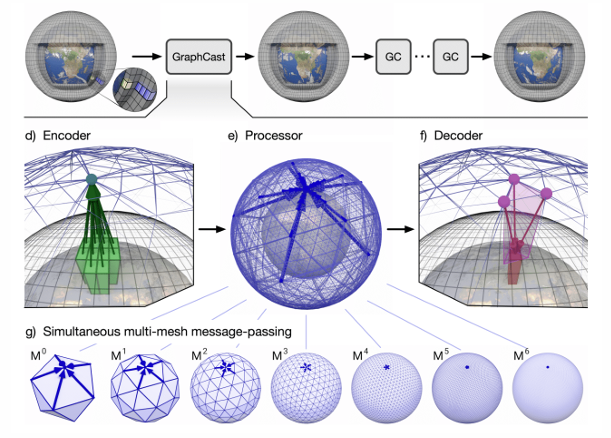
\includegraphics[width=0.6\textwidth]{Immagini/Screenshot 2026-11-10 174155.png} 
% \end{figure}


% \begin{itemize}
%     \item modella una sequenza temporale
%     \item usa il layar message-passing delle GNN 
%     \item viene addestrato su decenni di dati meteo;
%     \item predice lo stato atmosferico successivo.
% \end{itemize}

% \subsubsection{Mesh a diverse risoluzioni}

% GraphCast utilizza più mesh icosaedriche con risoluzioni di grana
% differenti:

% \begin{itemize}
%     \item \textbf{Mesh grossolane}: catturano il contesto
%     meteorologico globale.
%     \item \textbf{Mesh fini}: rappresentano meglio
%     i fenomeni meteorologici locali.
% \end{itemize}

 
\textbf{GraphCast} (DeepMind, 2023; Lam et al., \emph{Science}) è un modello
all'avanguardia per le previsioni meteo a medio termine. L'atmosfera è un grafo:
\begin{itemize}
  \item \textbf{nodi}: punti di una griglia su una mesh sferica (icosaedrica);
  \item \textbf{archi}: collegano posizioni spazialmente adiacenti;
  \item \textbf{feature dei nodi}: variabili meteorologiche (vento, temperatura,
        pressione, \dots).
\end{itemize}
\textbf{Architettura.} Modella una sequenza temporale (prevede stati futuri), usa
layer GNN a message passing ed è addestrato su decenni di dati meteo. Dallo stato
attuale predice lo stato successivo, e le previsioni a più giorni si ottengono
\emph{ripetendo} il passo (rollout). La struttura a blocchi è
\emph{encoder, processor, decoder}.

\begin{figure}[H] 
\centering
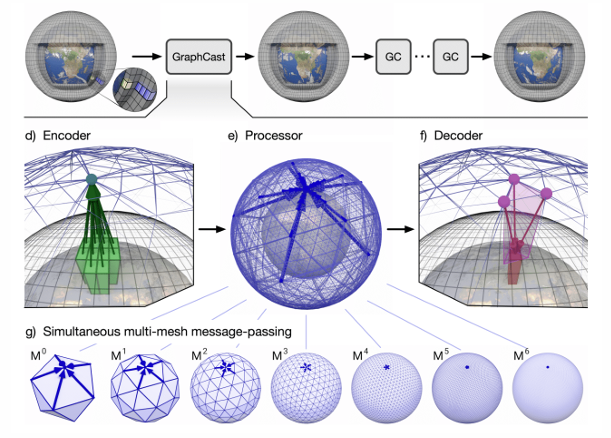
\includegraphics[width=0.6\textwidth]{Immagini/Screenshot 2026-11-10 174155.png} 
\end{figure}
 
\textbf{Mesh a più risoluzioni.} L'atmosfera è rappresentata da un insieme di
mesh icosaedriche a risoluzioni diverse ($M^0,\dots,M^6$): le mesh \textbf{grosse}
danno il contesto globale, quelle \textbf{fini} catturano i fenomeni meteorologici
locali. Il message passing sulle mesh avviene in modo simultaneo.
 
\textbf{Risultati.} Sulle previsioni a 10 giorni GraphCast è competitivo con i
modelli tradizionali basati sulla fisica come HRES, il principale sistema
operativo deterministico al mondo, con \textbf{inferenza molto più veloce}.

\begin{osservazione} GraphCast dimostra come le GNN
possano essere applicate a sistemi complessi e dinamici,
utilizzando un grafo per rappresentare le relazioni
spaziali e prevedere la loro evoluzione nel tempo.
\end{osservazione}
 
%---------------------------------------------------------------------
\subsection{Conclusioni e domande da orale}
%---------------------------------------------------------------------
 
Le GNN estendono le reti neurali ai dati a grafo usando le feature dei nodi e la
topologia. Operano per message passing: i nodi aggregano le informazioni dei
vicini per aggiornare le proprie rappresentazioni. GCN, GAT e GATv2 differiscono
nel modo di aggregare e pesare i vicini. Servono per node classification, link
prediction e graph classification, con applicazioni in reti sociali, biologia,
raccomandazione e altro. Restano aperti: scalabilità, over-smoothing,
interpretabilità, grafi dinamici.
 
\begin{enumerate}[label=\textbf{D\arabic*.}, leftmargin=*]
  \item \textbf{Perché la CNN non va bene su un grafo qualsiasi?}\\
  Assume vicinati di forma fissa e invarianza alle traslazioni. Su un grafo i
  nodi hanno gradi diversi e nessun ordine naturale.
  \item \textbf{Cos'è il message passing?}\\
  Ogni nodo aggrega gli embedding dei vicini con una funzione invariante
  all'ordine e poi li trasforma con una rete neurale.
  \item \textbf{Scrivere un layer GCN e spiegare i simboli.}\\
  $\mathbf{H}^{(\ell)}=\sigma(\hat{D}^{-1/2}\hat{A}\hat{D}^{-1/2}\mathbf{H}^{(\ell-1)}\mathbf{W}^{(\ell)})$, con
  $\hat{A}=A+I$, $\hat{D}$ dei gradi di $\hat{A}$, $\mathbf{W}$ appresa.
  \item \textbf{A cosa servono self-loop e normalizzazione?}\\
  Il self-loop conserva le feature del nodo; la normalizzazione evita che i nodi
  di grado alto producano valori più grandi.
  \item \textbf{Come si arriva alla GCN dal Laplaciano?}\\
  Filtro spettrale $Ug(\Lambda)U^\top x$ $\to$ polinomio di Chebyshev (niente
  autovettori) $\to$ grado 1 e $\lambda_{\max}\approx2$ $\to$ $\theta(I+S)x$ $\to$
  rinormalizzazione con self-loop, $\hat{S}$.
  \item \textbf{La sostituzione di $I+S$ con $\hat{S}$ è un'uguaglianza?}\\
  No, è un cambio di operatore. $\hat{S}$ ha autovalori di modulo al più 1 e non
  amplifica con la propagazione.
  \item \textbf{Cosa vede un nodo dopo $L$ layer?}\\
  I nodi a distanza al più $L$ hop.
  \item \textbf{Trasduttivo o induttivo?}\\
  Trasduttivo: stesso grafo in training e test, etichette solo su alcuni nodi.
  Induttivo: nodi o grafi nuovi nel test.
  \item \textbf{Come si passa da embedding di nodi a una classe del grafo?}\\
  Con un global pooling (media o attention) e un MLP finale.
  \item \textbf{Cosa aggiunge la GAT?}\\
  Pesi $\alpha_{ij}$ appresi per ogni arco, con softmax sui vicini.
  \item \textbf{Perché la GAT ha attention statica e come la corregge GATv2?}\\
  Il punteggio è somma di un termine su $i$ e uno su $j$ dentro una funzione
  monotona, quindi il ranking dei vicini non dipende da $i$. GATv2 applica
  $\mathbf{a}$ dopo la non-linearità.
  \item \textbf{Come funziona GraphCast?}\\
  GNN su mesh icosaedriche a più risoluzioni; predice lo stato successivo e
  fa il rollout fino a 10 giorni.
\end{enumerate}

\section{Autoencoder}

\subsection{Apprendimento non supervisionato}

Nel \textbf{supervised learning} il dataset contiene coppie $(\mathbf{x},y)$:
un dato e la sua etichetta. Si impara una funzione che, dato un nuovo input,
prevede $y$ (ad esempio la classificazione di immagini).

Nel \textbf{unsupervised learning} sono disponibili solo gli input
$\mathbf{x}$, senza etichette. Il modello deve trovare da solo regolarità e
struttura nei dati.

\subsubsection{Perché serve}
\begin{itemize}
  \item \textbf{Disponibilità dei dati:} i modelli profondi hanno molti
        parametri e, per evitare l'overfitting, servono molti dati. Raccogliere
        dati non etichettati costa molto meno: le etichette richiedono tempo,
        lavoro umano e competenze specifiche.
  \item \textbf{Struttura senza etichette:} i dati hanno regolarità anche senza
        supervisione. Dato un campione di una variabile casuale $\mathbf{x}$,
        l'algoritmo impara, in modo esplicito o implicito, la distribuzione
        $p(\mathbf{x})$ o alcune sue proprietà. Ad esempio, immagini di classi
        diverse condividono strutture visive anche se le classi non sono note.
  \item \textbf{Pre-training:} l'apprendimento non supervisionato si può usare
        prima di un compito supervisionato.
  \begin{itemize}
    \item \textbf{Ottimizzazione:} i parametri partono da una regione migliore
          di quella di un'inizializzazione casuale.
    \item \textbf{Regolarizzazione:} imparare prima la struttura generale dei
          dati riduce il rischio di adattarsi troppo agli esempi etichettati.
  \end{itemize}
\end{itemize}

Questi vantaggi contano nel \textbf{transfer learning} e nella
\textbf{domain adaptation}: una rappresentazione appresa su dati disponibili
viene riusata su un nuovo compito o su un dominio diverso.

%---------------------------------------------------------------------
\subsection{Learning representations}
%---------------------------------------------------------------------

\subsubsection{Lo spazio dei dati}
Prendiamo MNIST: immagini di cifre $28\times 28$. Anche con un solo bit per
pixel, un'immagine ha $28\cdot 28=784$ valori e le immagini possibili sono
$2^{784}\approx 10^{236}$. Quasi nessuna è una cifra: le immagini reali
occupano una parte minuscola di $\{0,1\}^{784}$.

Lo stesso vale per il linguaggio: una sequenza di lettere scelte a caso ha
probabilità praticamente nulla di essere un testo sensato.

\subsubsection{Manifold assumption}
\begin{definizione}[Manifold assumption]
I dati reali stanno approssimativamente su una varietà (\emph{manifold}) con
dimensione molto più bassa di quella dello spazio di input.
\end{definizione}

Un dato ha molte variabili, ma la sua variabilità dipende da pochi fattori.
Una cifra è descritta da 784 pixel, ma cambia solo in base a quale cifra è,
inclinazione, spessore del tratto, posizione e stile. Modificare i pixel
indipendentemente quasi mai dà un'immagine plausibile.

\textbf{QUINDI:} conviene descrivere il dato con coordinate sulla varietà, non
con tutte le coordinate di $\mathbb{R}^{N}$.

\subsubsection{Cos'è una buona rappresentazione}
Dato $\mathbf{x}$, si cerca una nuova rappresentazione $\mathbf{h}$ che
conservi più informazione possibile su $\mathbf{x}$, sotto qualche vincolo o
penalizzazione. Senza vincolo $\mathbf{h}$ potrebbe copiare l'input e non
semplificare nulla.

\begin{itemize}
  \item \textbf{Task-specific:} costruita per un compito successivo
        (ad esempio la classificazione).
  \item \textbf{Task-agnostic:} descrive la struttura generale dei dati, senza
        legarsi a un compito.
\end{itemize}

\textbf{Criteri tipici:}
\begin{itemize}
  \item \textbf{Dimensionalità ridotta:} $\mathbf{h}$ ha meno componenti di
        $\mathbf{x}$ e tiene solo l'informazione importante.
  \item \textbf{Sparsa:} per quasi ogni input, la maggior parte delle
        componenti di $\mathbf{h}$ è zero o molto piccola. Il vettore può
        essere grande, ma poche componenti sono attive per ogni esempio.
  \item \textbf{Fattori indipendenti:} le componenti di $\mathbf{h}$ sono
        statisticamente indipendenti e descrivono aspetti diversi del dato,
        senza ripetere informazione correlata.
\end{itemize}

\begin{importante}[Da saper dire a voce]
I dati reali occupano una parte piccolissima dello spazio di input e hanno pochi
fattori di variazione (manifold assumption). L'apprendimento non supervisionato
cerca una rappresentazione $\mathbf{h}$ che li catturi: compatta, sparsa o a
fattori indipendenti, e utile anche senza etichette.
\end{importante}

%---------------------------------------------------------------------
\subsection{Riduzione della dimensionalità e PCA}
%---------------------------------------------------------------------

\subsubsection{Dimensionality reduction}
Le tecniche di \textbf{dimensionality reduction} trasformano dati ad alta
dimensione in rappresentazioni con meno componenti. Se il modello è costretto
a comprimere l'input, deve scegliere quali informazioni tenere: elimina le
ridondanze e prova a perdere il meno possibile di quanto è rilevante. Le
componenti ridotte possono inoltre dipendere meno tra loro di quelle originali.

\subsubsection{Principal Component Analysis (PCA)}
La \textbf{PCA} è un algoritmo non supervisionato che semplifica i dati "schiacciandoli"
lungo linee dritte e perpendicolari (una trasformazione \emph{lineare e ortogonale}):
\[
\mathbf{x} \text{ (dato originale)} \longmapsto \mathbf{z} \text{ (dato compresso)}.
\]
$\mathbf{z}$ sta nel sottospazio generato dalle componenti principali,
che sono le direzioni trovate dalla PCA, in base all distirubuzione dei dati. e sono ortogonali 
tra loro. I dati sono descritti da poche direzioni, quelle ritenute più importanti.

\textbf{Limite.} La PCA funziona bene quando i dati stanno formano a una varietà
\emph{lineare}. Se i dati formano curve, spirali o raggruppamenti complessi 
le dipendenze tra le feature sono non lineari, una trasformazione lineare non basta e 
servono modelli più flessibili, cioè reti neurali.

\begin{figure}[H]
\centering
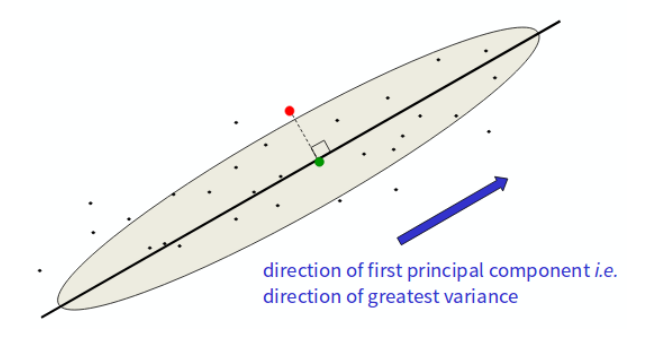
\includegraphics[width=0.4\textwidth]{Immagini/Screenshot 2026-11-13 121038.png}
\caption{PCA: la prima componente principale è la direzione di massima varianza.
Il punto rosso è l'originale(2 coordinate), il verde la sua proiezione sulla retta.}
\end{figure}

\subsubsection{Una rete che ritrova la PCA}
È possibile usare una \textbf{rete neurale con un "collo di bottiglia" (bottleneck)} per ottenere lo stesso 
risultato della PCA. Si chiede alla rete di prendere un input $\mathbf{x}$, comprimerlo in uno strato 
nascosto più piccolo $\mathbf{h}$, e poi usarlo per ricostruire il dato originale in uscita come $\mathbf{r}$:
\[
\mathbf{x} \longrightarrow \mathbf{h} \longrightarrow \mathbf{r}
\]

\begin{figure}[H]
\centering
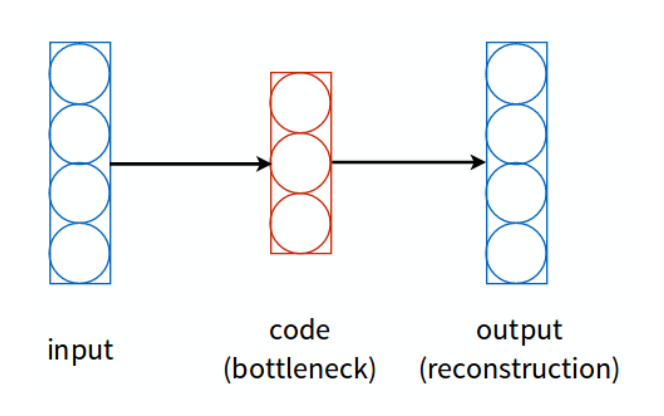
\includegraphics[width=0.5\textwidth]{Immagini/Screenshot 2026-11-13 121046.png}
\caption{Rete con strato a bottleneck: input, codice e output (ricostruzione).}
\end{figure}

Se manteniamo gli strati della rete \textbf{puramente lineari}
e la addestriamo per minimizzare l'errore di ricostruzione, le unità nascoste imparano 
a schiacciare i dati nello \textbf{stesso identico sottospazio generato dalla PCA}, ma 
cambiando la base, infatti i pesi trovati non sono più per forza ortogonali


\begin{osservazione}
Questa rete è già un autoencoder: se si aggiungono non linearità(funzioni di attivazione), può
apprendere rappresentazioni che la PCA non raggiunge.
\end{osservazione}

%---------------------------------------------------------------------
\subsection{Definizione di autoencoder}
%---------------------------------------------------------------------

Un \textbf{autoencoder} è una rete feed-forward addestrata a copiare l'input
in output. Lo scopo è ma ottenere una rappresentazione intermedia ($h$) che conservi 
le caratteristiche importanti dei dati.

\begin{figure}[H]
\centering
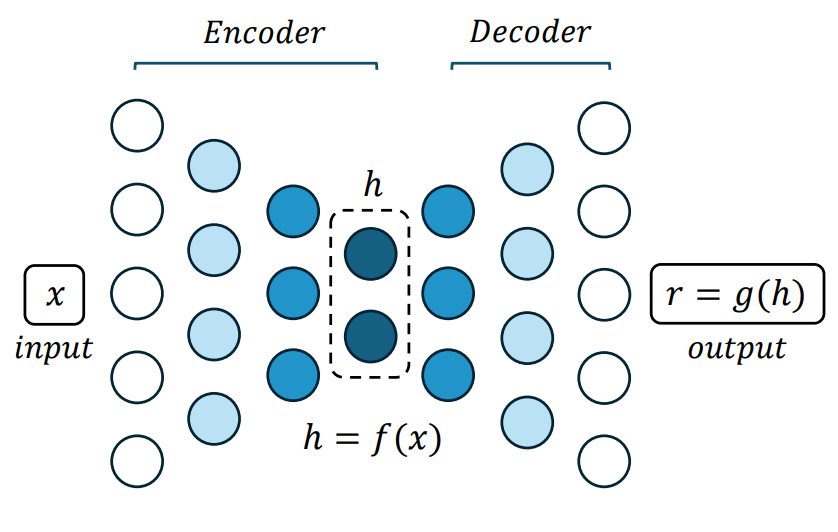
\includegraphics[width=0.5\textwidth]{Immagini/Screenshot 2026-11-13 123824.png}
\end{figure}


Ha due parti:
\begin{itemize}
  \item \textbf{Encoder.} Produce un codice che contiene le informazioni più
salienti. Non deve mantenere ogni dettaglio: deve bastare per ricostruire il
dato in modo soddisfacente.
  \item \textbf{Decoder.} Parte da $\mathbf{h}$ e produce $\mathbf{r}$, che deve
essere il più vicina possibile a $\mathbf{x}$. L'errore di ricostruzione
misura la differenza tra i due, e l'addestramento lo riduce.
\end{itemize}
\[
\mathbf{h}=f(\mathbf{x}),\qquad
\mathbf{r}=g(\mathbf{h})=g(f(\mathbf{x})).
\]
$\mathbf{x}$ è il dato originale, $\mathbf{h}$ è il \textbf{codice}
(rappresentazione latente) e $\mathbf{r}$ è la ricostruzione.

\textbf{Varietà non lineari.} Inserendo strati non lineari e usando più layer,
 encoder e decoder rappresentano trasformazioni molto più ricche di una semplice proiezione 
 lineare (come la PCA). L'encoder porta i dati dallo spazio originale a coordinate latenti, 
 mentre il decoder fa il passaggio inverso. In questo modo la rete riesce a descrivere e
ricostruire dati complessi che stanno su una \emph{varietà non lineare}, o vicino a essa.

\subsubsection{Overfitting: la funzione identità}
La rete potrebbe imparare
\[
g(f(\mathbf{x}))=\mathbf{x},
\]
cioè ricostruire perfettamente l'input senza aver imparato nulla di utile. Succede
soprattutto se encoder e decoder hanno troppa capacità, per esempio con un
codice di dimensione maggiore dell'input: il dato si copia senza comprimerlo.

\textbf{QUINDI:} una ricostruzione perfetta non garantisce una buona
rappresentazione. Servono vincoli.

%---------------------------------------------------------------------
\subsection{Undercomplete autoencoder}
%---------------------------------------------------------------------

Il primo vincolo è imporre che il codice abbia dimensione minore dell'input:
\[
\dim(\mathbf{h})<\dim(\mathbf{x}).
\]
Il codice è un collo di bottiglia: la rete deve rappresentare l'input con meno
componenti. \textit{OBIETTIVO:} minimizzare una loss di ricostruzione
\[
\boxed{\mathcal{L}\big(\mathbf{x},g(f(\mathbf{x}))\big)}
\]
che penalizza la differenza tra $\mathbf{x}$ e $\mathbf{r}=g(f(\mathbf{x}))$.
Una scelta è l'errore quadratico medio,
\[
\operatorname{MSE}(\mathbf{x},\mathbf{r})=\frac{1}{N}\sum_{i=1}^{N}(x_i-r_i)^2,
\]
con $N$ numero di componenti del dato.

Poiché il codice (bottleneck) ha meno dimensioni dell'input, la rete non ha lo spazio fisico per conservare o
gni dettaglio. È quindi costretta selezionare e salvare i 
\textbf{fattori di variazione più importanti} per ricostruire i dati.

L'\textbf{undercomplete autoencoder} è una generalizzazione non lineare della PCA:
\begin{itemize}
    \item La \textbf{PCA} si limita ad apprendere una proiezione lineare.
    \item L'\textbf{Autoencoder} (grazie agli strati non lineari) apprende una rappresentazione compressa 
    molto più ricca e flessibile.
\end{itemize}

\vspace{0.2cm}
\textbf{Il limite: la dimensionalità ridotta non basta.} 
Avere un codice più piccolo dell'input non garantisce, da solo, che la rete estragga feature sensate. 
Se l'encoder e il decoder hanno \emph{troppa capacità} (sono reti troppo grandi o complesse), 
riescono comunque a imparare a memoria i dati, producendo una copia poco significativa (overfitting).

\textbf{La soluzione:} Per arginare il problema si introducono gli \textbf{Autoencoder Regolarizzati} che 
aggiungono \emph{vincoli aggiuntivi nella loss function} per guidare l'apprendimento

%---------------------------------------------------------------------
\subsection{Autoencoder regolarizzati}
%---------------------------------------------------------------------
Con la regolarizzazione la loss non valuta più solo la ricostruzione, ma ha un
termine che incoraggia proprietà della rappresentazione. L'autoencoder può
copiare l'input solo in modo approssimato, quindi deve scegliere cosa
conservare e finisce per apprendere la struttura della distribuzione dei dati.

Tre tipologie: \textit{sparse}, \textit{denoising}, \textit{contractive}.

%---------------------------------------------------------------------
\subsection{Sparse autoencoder}
%---------------------------------------------------------------------

Uno \textbf{sparse autoencoder} è un autoencoder la cui funzione di
addestramento include una penalizzazione aggiuntiva che incoraggia
la sparsità del codice $h$.
$\mathbf{h}$:
\[
\boxed{
\mathcal{L}_{SAE}=D\big(\mathbf{x},g(f(\mathbf{x}))\big)+\lambda\,\|\mathbf{h}\|_1
}
\qquad
\|\mathbf{h}\|_1=\sum_j|h_j|.
\]
\begin{itemize}
  \item $D(\mathbf{x},g(f(\mathbf{x})))$: errore di ricostruzione;
  \item $\|\mathbf{h}\|_1$: penalizzazione delle attivazioni del codice;
  \item $\lambda$: peso della penalizzazione rispetto alla ricostruzione.
\end{itemize}
%Nelle slide il termine è scritto $\lambda|\mathbf{h}|$. La norma $L_1$ è la
%scelta usuale, ma la forma esatta dipende dall'implementazione.
\begin{figure}[H]
\centering
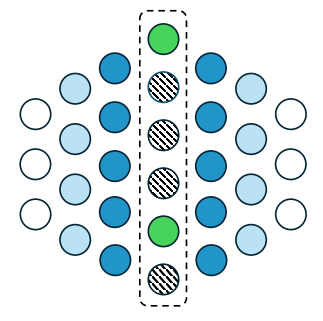
\includegraphics[width=0.2\textwidth]{Immagini/Screenshot 2026-11-13 153836.png}
\end{figure}
\textbf{Rappresentazione overcomplete.} Lo sparse autoencoder può avere
$\dim(\mathbf{h})>\dim(\mathbf{x})$ senza imparare l'identità, perché la
penalizzazione limita quante componenti sono attive insieme. Il codice ha molte
dimensioni disponibili, ma ne usa poche per ogni input.

\textbf{Dizionario di caratteristiche.} Si può vedere come l'apprendimento di
un dizionario di concetti elementari. Dato un segnale, il modello cerca una
lista breve di elementi del dizionario che lo descriva bene. Il dizionario può
essere molto più grande dell'input; $\mathbf{h}$ ha una componente per
elemento, e solo poche sono attive per un dato esempio. I dati sono descritti
da poche caratteristiche ricorrenti.

\textbf{Utilizzo.} Si usa soprattutto per apprendere feature da riusare in un
altro compito, come la classificazione. L'autoencoder non classifica:
costruisce una rappresentazione che viene data a un modello dedicato.

%---------------------------------------------------------------------
\subsection{Denoising autoencoder (DAE)}
%---------------------------------------------------------------------

Il DAE è addestrato a ricostruire l'input originale partendo da una versione
\emph{corrotta}. All'encoder non si dà $\mathbf{x}$ ma $\tilde{\mathbf{x}}$,
ottenuto con una perturbazione:
\[
\tilde{\mathbf{x}}\longrightarrow\mathbf{h}\longrightarrow\mathbf{r}\approx\mathbf{x}.
\]
Dove r deve essere simile al dato originale, quindi il target è $\mathbf{x}$, non $\tilde{\mathbf{x}}$:
\[
\boxed{\mathcal{L}_{DAE}=D\big(\mathbf{x},g(f(\tilde{\mathbf{x}}))\big)}
\]
\[
\begin{aligned}
\text{Autoencoder standard:}\quad&D\big(\mathbf{x},g(f(\mathbf{x}))\big)\\
\text{Denoising autoencoder:}\quad&D\big(\mathbf{x},g(f(\tilde{\mathbf{x}}))\big)
\end{aligned}
\]

\textbf{Come si corrompe l'input.} Con rumore gaussiano bianco o con dropout.
Nel caso gaussiano
\[
\tilde{\mathbf{x}}\sim\mathcal{N}(\mathbf{x},\sigma^2\mathbf{I}),
\]
dove $\sigma^2$ controlla la varianza del rumore e $\mathbf{I}$ è la matrice
identità, quindi si aggiunge una perturbazione casuale.

\textbf{Perché impara feature robuste.} Se la rete ricevesse sempre il dato
da ricostruire, potrebbe copiarlo. Con l'input alterato deve capire quali
caratteristiche sono stabili e quali variazioni sono rumore, quindi impara la
struttura dei dati.

\subsubsection{Interpretazione geometrica}

I dati validi stanno vicino a una varietà; $\mathbf{x}$ è sulla curva,
$\tilde{\mathbf{x}}$ può essere fuori. Il DAE impara a riportare il punto
corrotto verso la regione dei dati originali:
\[
\tilde{\mathbf{x}}\longrightarrow\mathbf{r}\approx\mathbf{x}.
\]
Sapendo, per tanti punti vicini alla varietà, dove ricostruirli, il modello
apprende in modo implicito la sua geometria. Le slide lo descrivono come
l'apprendimento di un \textbf{vector field} diretto verso le regioni a
probabilità più alta, quindi della struttura di $p_{\text{data}}(\mathbf{x})$.
\begin{figure}[H]
\centering
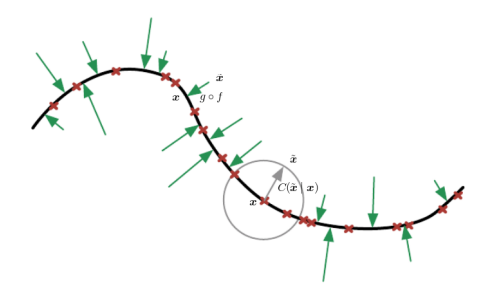
\includegraphics[width=0.4\textwidth]{Immagini/Screenshot 2026-11-13 154722.png}
\end{figure}

\subsubsection{Anomaly detection con un DAE}
\begin{enumerate}
  \item \textbf{Training:} si addestra il DAE solo su dati normali, in versione
        rumorosa, con target il campione normale originale.
  \item \textbf{Inferenza:} dato un nuovo campione $\mathbf{x}$, si calcola
        la ricostruzione $\mathbf{r}$.
  \item \textbf{Errore:} $e(\mathbf{x})=\|\mathbf{x}-\mathbf{r}\|_2$.
  \item \textbf{Decisione:} se l'errore è alto, il campione è segnalato come
        possibile anomalia.
\end{enumerate}
Un campione anomalo può non stare sulla varietà appresa e avere caratteristiche
mai viste, quindi la ricostruzione è peggiore. Un errore alto è una
segnalazione di anomalia \emph{potenziale}, non una prova.

%---------------------------------------------------------------------
\subsection{Contractive autoencoder (CAE)}
%---------------------------------------------------------------------

Il CAE ricostruisce l'input dal codice e rende anche il codice poco sensibile
alle piccole variazioni dell'input.
La funzione di costo è formata da due termini in competizione:
\[
\mathcal{L}_{CAE}=D\big(\mathbf{x},g(f(\mathbf{x}))\big)
+\lambda\left\|\frac{\partial f(\mathbf{x})}{\partial\mathbf{x}}\right\|^2
\]
Il primo termine è l'errore di ricostruzione. Il secondo penalizza la
sensibilità dell'encoder: la matrice
\[
\mathbf{J}_f(\mathbf{x})=\frac{\partial f(\mathbf{x})}{\partial\mathbf{x}}
\]

\begin{itemize}
    \item Il primo termine $D(\dots)$ è l'\textbf{errore di ricostruzione}, che spinge la rete a guardare i 
    dettagli per copiare bene l'input.
    \item Il secondo termine penalizza la \textbf{sensibilità dell'encoder}. La matrice
    \[ \mathbf{J}_f(\mathbf{x})=\frac{\partial f(\mathbf{x})}{\partial\mathbf{x}} \]
    è lo \textbf{Jacobiano} dell'encoder: misura quanto "sfarfalla" il codice $\mathbf{h}$ al minimo 
    variare dell'input $\mathbf{x}$. Inserire la sua norma nella loss forza la rete a non cambiare se 
    l'input cambia di poco. $\lambda$ ne regola l'importanza.
\end{itemize}

\textbf{Effetto pratico:} 
Minimizzando il termine Jacobiano, l'encoder impara a non reagire alle piccole perturbazioni. 
Riduce i gradi di libertà e mantiene solo le variazioni davvero necessarie per ricostruire il dato.

\begin{figure}[H]
\centering
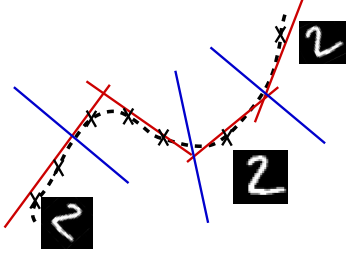
\includegraphics[width=0.4\textwidth]{Immagini/Screenshot 2026-11-13 154734.png}
\caption{Direzioni importanti (rosse) e non importanti (blu).}
\end{figure}

\textbf{Direzioni importanti e non importanti.}
\begin{itemize}
    \item \textbf{Importanti (Linee Rosse):} Lungo queste direzioni i dati di training variano realmente
     (es. il numero 2 si inclina o si allunga). Per colpa del termine di ricostruzione, qui 
     l'encoder \textbf{deve restare sensibile}. Queste linee corrispondono ai \textbf{piani tangenti} alla varietà.
    \item \textbf{Non importanti (Linee Blu):} Sono direzioni in cui i dati veri non 
    variano (es. rumore casuale che "butta fuori" il dato dal sentiero). Qui vince lo Jacobiano: 
    l'encoder \textbf{ignora le variazioni} e diventa cieco.
\end{itemize}



\textbf{Perché ``contractive''.} Il CAE mappa un intorno di punti di input in
un intorno più piccolo nello spazio delle rappresentazioni: punti vicini
producono codici più simili.
----------------------------------------------------
Il CAE mappa un intero intorno di punti di input (il dato vero + tutte le sue varianti rumorose lungo le linee blu) 
in un intorno molto più piccolo nello spazio latente. In pratica, \textbf{contrae} o schiaccia le perturbazioni, 
facendo sì che punti vicini producano codici quasi identici.

\textbf{Relazione con la varietà.} Come il DAE, il CAE dà informazioni sulla
struttura della varietà. Le slide dicono che conosce i \textbf{piani tangenti}
nei punti considerati: la penalizzazione distingue le direzioni in cui la
rappresentazione deve variare (lungo la varietà) da quelle in cui può restare
stabile.
------------------------------
Così come il Denoising Autoencoder (DAE), anche il CAE mappa la struttura geometrica dei dati.
 Costringendo la rete a essere sensibile solo lungo certe direzioni, il CAE impara esplicitamente 
 i \textbf{piani tangenti} (le linee rosse) alla varietà dei dati in ogni punto considerato.

\subsubsection{DAE e CAE}
Entrambi puntano a rappresentazioni robuste a piccole perturbazioni.
\begin{itemize}
  \item \textbf{DAE:} la corruzione è reale, applicata all'input. La
        robustezza viene dal compito di denoising.
  \item \textbf{CAE:} la penalizzazione sullo Jacobiano è nella loss. La
        robustezza è imposta in modo esplicito.
\end{itemize}

%---------------------------------------------------------------------
\subsection{Confronto tra gli autoencoder}
%---------------------------------------------------------------------

Tutte le architetture ricostruiscono l'input, ma con vincoli diversi per
evitare la copia.

\begin{center}
\renewcommand{\arraystretch}{1.35}
\begin{tabular}{|p{2.6cm}|p{4.6cm}|p{7.2cm}|}
\hline
\textbf{Modello} & \textbf{Vincolo} & \textbf{Effetto sulla rappresentazione} \\
\hline
Undercomplete & $\dim(\mathbf{h})<\dim(\mathbf{x})$
& costringe a comprimere e a tenere i fattori di variazione più salienti \\
\hline
Sparse & penalizzazione delle attivazioni di $\mathbf{h}$
& il codice può essere overcomplete, ma per ogni input sono attive poche
componenti \\
\hline
Denoising & ricostruire $\mathbf{x}$ da $\tilde{\mathbf{x}}$
& rimuove il rumore e impara feature robuste e la struttura dei dati \\
\hline
Contractive & penalizzazione dello Jacobiano dell'encoder
& il codice cambia poco per piccole perturbazioni dell'input \\
\hline
\end{tabular}
\end{center}

\begin{importante}[Da saper dire a voce]
Un autoencoder ricostruisce l'input attraverso un codice latente, ma senza
vincoli può imparare l'identità. L'undercomplete comprime il codice; lo sparse
penalizza le attivazioni e ammette un codice overcomplete; il denoising
ricostruisce l'originale da una versione corrotta e impara a riportare i punti
sulla varietà; il contractive penalizza lo Jacobiano dell'encoder per avere un
codice stabile. Il passo successivo sono i Variational Autoencoder (VAE): dopo
la rappresentazione latente, si modella anche la sua distribuzione.
\end{importante}

%=====================================================================
\section{Variational Autoencoder}
%=====================================================================

%---------------------------------------------------------------------
\subsection{Modelli generativi}
%---------------------------------------------------------------------

Il \textit{generative modeling} è un'area del Machine Learning che studia modelli capaci di descrivere la 
distribuzione di probabilità dei dati:
\[p(x),\]
dove $x$ rappresenta un dato osservato e può appartenere a uno spazio anche 
molto grande e ad alta dimensionalità. Se $x$ è un'immagine:
\begin{itemize}
    \item immagini realistiche, simili a quelle presenti nel dataset, dovrebbero avere probabilità elevata;
    \item immagini simili a rumore casuale dovrebbero avere probabilità molto bassa.
\end{itemize}

Lo scopo non è classificare dati già visti, ma imparare $p(\mathbf{x})$ per
\textbf{generare nuovi esempi} simili a quelli del dataset, senza copiarli.

\begin{osservazione}
  \textbf{Collegamento con gli autoencoder.} DAE e CAE imparano in modo implicito
  la struttura di $p(\mathbf{x})$, ma non è facile \textbf{campionare} nuovi dati
  da loro. L'idea dei modelli a variabili latenti è descrivere la distribuzione
  complessa dei dati con una distribuzione più semplice, introducendo variabili
  nascoste.
\end{osservazione}

%---------------------------------------------------------------------
\subsection{Latent variable models}
%---------------------------------------------------------------------

\subsubsection{Variabili osservabili e latenti}
Un modello a variabili latenti mette in relazione:
\begin{itemize}
  \item le variabili \textbf{osservabili} $\mathbf{x}$: i dati che si misurano;
  \item le variabili \textbf{latenti} $\mathbf{z}$: fattori nascosti che non si
        osservano ma contribuiscono a spiegare i dati.
\end{itemize}

\begin{figure}[H]
\centering
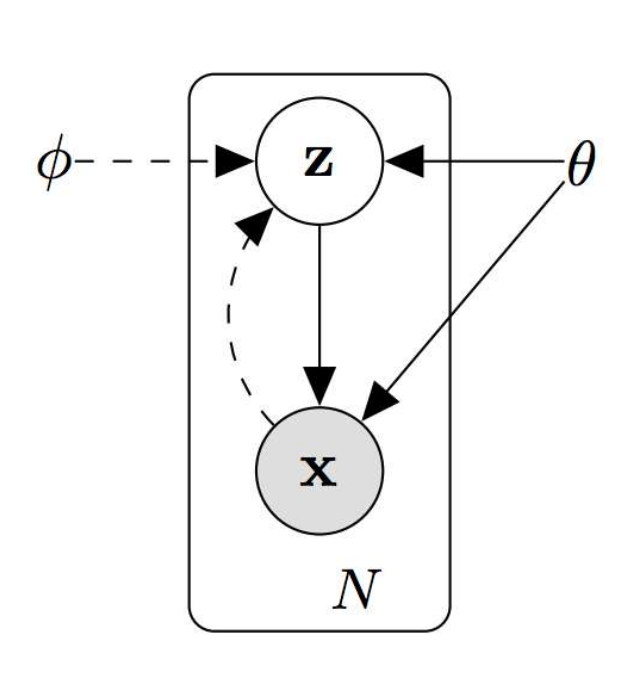
\includegraphics[width=0.3\textwidth]{Immagini/Screenshot 2026-11-15 101435.png}
\caption{Direzioni importanti (rosse) e non importanti (blu).}
\end{figure}

Nel contesto generativo, vogliamo produrre un dato $x$. Per farlo, immaginiamo
che esista una rappresentazione latente $z$ dalla quale il dato viene generato:
\[
z \longrightarrow x.
\]
il modello parte da una
descrizione compatta(interna $z$) e produce un'osservazione $x$.

\textbf{Esempio: meteo.} Si misurano temperatura, umidità e velocità del vento
($\mathbf{x}$). Questi valori vengono influenzati anche da fattori fisici non misurati: gradienti
di pressione, profili di temperatura in funzione dell'altitudine, vapore acqueo
e densità delle nuvole. Sono le variabili latenti $\mathbf{z}$. Una variabile
latente può quindi essere una quantità fisica reale, solo non osservata.

\subsubsection{Distribuzione dei dati: marginalizzazione della variabile latente}
Vogliamo descrivere la probabilità di osservare un dato $x$, tenendo conto
che esso può essere stato generato anche grazie a valori della variabile latente $z$.

La distribuzione congiunta può essere scritta usando la regola della probabilità condizionata:
\[
p(\mathbf{x},\mathbf{z})=p(\mathbf{x}\mid\mathbf{z})\,p(\mathbf{z}).
\]
Per ottenere la distribuzione dei soli dati osservabili si elimina $\mathbf{z}$ con la
\textbf{marginalizzazione}:
\[
p(\mathbf{x})=\int p(\mathbf{x},\mathbf{z})\,d\mathbf{z}
=\int p(\mathbf{x}\mid\mathbf{z})\,p(\mathbf{z})\,d\mathbf{z}
\]
\begin{itemize}
  \item $p(\mathbf{z})$ è la \textbf{prior}: i valori di $\mathbf{z}$ plausibili
        prima di osservare $\mathbf{x}$ (nel VAE viene fissata come una 
        gaussiana standard $\mathcal{N}(\mathbf{0}, \mathbf{I})$);
  \item $p(\mathbf{x}\mid\mathbf{z})$ descrive come si genera il dato($x$) conoscendo
        $\mathbf{z}$;
  \item $p(\mathbf{x})$ è la distribuzione marginale dei dati considerando le cause latenti.
  \end{itemize}

Con $\mathbf{z}$ discreta l'integrale diventa una somma,
$p(\mathbf{x})=\sum_{\mathbf{z}}p(\mathbf{x}\mid\mathbf{z})p(\mathbf{z})$.

\noindent\textbf{Perché è difficile.} Nei modelli complessi questo integrale è 
\textbf{intrattabile} (\emph{intractable}): poiché $\mathbf{z}$ vive 
in uno spazio continuo ad alta dimensione e non esiste un'espressione in forma chiusa 
facile da valutare analiticamente.

\subsubsection{Prima soluzione: approssimazione Monte Carlo}

L'integrale può essere riscritto come valore atteso rispetto alla prior,
\[
    p(\mathbf{x}) = \mathbb{E}_{\mathbf{z}\sim p(\mathbf{z})}\bigl[p(\mathbf{x} \mid \mathbf{z})\bigr],
\]
e quindi approssimato numericamente estraendo $K$ campioni casuali dalla prior e calcolando la media empirica:
\[
    p(\mathbf{x}) \approx \frac{1}{K}\sum_{k=1}^{K} p(\mathbf{x} \mid \mathbf{z}^{(k)}),
    \qquad \mathbf{z}^{(k)} \sim p(\mathbf{z})
\]

\begin{figure}[h!]
\centering
\begin{tikzpicture}[scale=0.9]

% --- GRAFICO SINISTRO: INTEGRALE CONTINUO ---
\begin{scope}[shift={(0,0)}]
    \node[align=center, font=\bfseries\small] at (2.1, 3.3) {Integrale continuo};
    \draw[->, thick] (0,0) -- (4.3,0) node[right] {$\mathbf{z}$};
    \draw[->, thick] (0,0) -- (0,2.4) node[above] {$p(\mathbf{x}\mid\mathbf{z})p(\mathbf{z})$};
    \foreach \x in {0.2, 0.35, ..., 3.9} {
        \pgfmathsetmacro{\y}{1.25 + 0.5*sin(deg(1.4*\x))}
        \draw[gray!65, thin] (\x, 0) -- (\x, \y);
    }
    \draw[very thick, blue!70!black, domain=0.1:4.0, samples=60] 
        plot (\x, {1.25 + 0.5*sin(deg(1.4*\x))});
    \node[align=center, font=\footnotesize] at (2.1, -0.6) 
        {Impossibile sommare su tutti\\gli infiniti valori di $\mathbf{z}$};
\end{scope}

% --- FRECCIA CENTRALE ---
\draw[->, very thick, dashed] (4.8, 1.2) -- (5.8, 1.2);

% --- GRAFICO DESTRO: APPROSSIMAZIONE MONTE CARLO ---
\begin{scope}[shift={(6.4,0)}]
    \node[align=center, font=\bfseries\small] at (2.1, 3.0) {Approssimazione\\Monte Carlo};
    \draw[->, thick] (0,0) -- (4.3,0) node[right] {$\mathbf{z}$};
    \draw[->, thick] (0,0) -- (0,2.4) node[above] {$p(\mathbf{x}\mid\mathbf{z})$};
    \foreach \x in {0.45, 0.9, 1.15, 1.85, 2.2, 3.1, 3.4, 3.85} {
        \pgfmathsetmacro{\y}{1.25 + 0.5*sin(deg(1.4*\x))}
        \draw[red!80!black, line width=1.5pt] (\x, 0) -- (\x, \y);
        \fill[red!80!black] (\x, \y) circle (1.5pt);
    }
    \draw[very thick, blue!70!black, domain=0.1:4.0, samples=60] 
        plot (\x, {1.25 + 0.5*sin(deg(1.4*\x))});
    \node[align=center, font=\footnotesize] at (2.1, -0.6) 
        {Media su $K$ campioni casuali\\$\mathbf{z}^{(k)} \sim p(\mathbf{z})$};
\end{scope}

\end{tikzpicture}
\end{figure}

La generalizzazione consiste in:
\begin{enumerate}
    \item estrarre un vettore latente dalla prior: $\mathbf{z}^{(k)} \sim p(\mathbf{z})$;
    \item generare (o valutare) l'osservazione corrispondente: $\mathbf{x} \sim p_\theta(\mathbf{x} \mid \mathbf{z}^{(k)})$;
    \item ripetere $K$ volte e applicare la media Monte Carlo.
\end{enumerate}
\subsubsection{Problemi dell'approssimazione Monte Carlo (campionamento dalla prior)}

Campionare direttamente dalla prior $p(\mathbf{z})$ è computazionalmente
\textbf{inefficiente}. La prior descrive quali valori di $\mathbf{z}$ sono plausibili
\emph{in generale} sull'intero dataset, senza sapere quale specifico dato $\mathbf{x}$
vogliamo spiegare. I campioni $\mathbf{z}^{(k)}$ cadono dove $p(\mathbf{z})$ è alta, e
questa zona non coincide in generale con quella in cui $p(\mathbf{x}\mid\mathbf{z})$ è grande.

Per l'osservazione corrente $\mathbf{x}$ la maggior parte dei campioni è quindi
irrilevante: produce $p(\mathbf{x}\mid\mathbf{z}^{(k)})\approx 0$ e non contribuisce alla
media. Solo pochi termini della somma sono significativi, perciò serve un numero
$K$ molto grande di campioni per ottenere una stima affidabile di $p(\mathbf{x})$.

\begin{figure}[H]
\centering
\begin{tikzpicture}[scale=0.9]
    \basefig{zona utile\\per $\mathbf{x}$}
    \campioniprior
    \node[align=center, font=\footnotesize] at (0.2,-1.0)
        {$\mathbf{z}^{(k)}\sim p(\mathbf{z})$: solo 1 campione su 8\\
         cade nella zona utile};
\end{tikzpicture}
\caption{Campioni estratti dalla prior $p(\mathbf{z})$ (curva nera) rispetto alla zona
rilevante per l'osservazione $\mathbf{x}$ (in arancione). La maggior parte dei campioni
(in grigio) cade dove $p(\mathbf{x}\mid\mathbf{z})\approx 0$ e non contribuisce alla stima.}
\end{figure}

\noindent\textbf{Idea della Variational Inference.} Per concentrare i campioni nella zona
utile introduciamo una distribuzione proposta $q_\phi(\mathbf{z}\mid\mathbf{x})$ (realizzata
dall'\textbf{Encoder}) che, \emph{dato} l'ingresso osservato $\mathbf{x}$, predice i valori
latenti $\mathbf{z}$ più plausibili per generarlo. In questo modo bastano pochi campioni
mirati per approssimare bene l'integrale.

%---------------------------------------------------------------------
\subsection{Inferenza variazionale}
%---------------------------------------------------------------------

La distribuzione utile è la \textbf{posterior} $p(\mathbf{z}\mid\mathbf{x})$:
quanto sono plausibili i valori di $\mathbf{z}$ \emph{dopo} aver osservato
$\mathbf{x}$. Per Bayes
\[
p(\mathbf{z}\mid\mathbf{x})=\frac{p(\mathbf{x}\mid\mathbf{z})\,p(\mathbf{z})}{p(\mathbf{x})}
\]
ma il denominatore $p(\mathbf{x})$ è proprio l'integrale intrattabile.

L'\textbf{inferenza variazionale} introduce una \emph{proposal distribution}
$q(\mathbf{z}\mid\mathbf{x})$, facile da valutare e da campionare, che approssima
la vera posterior. 

\textbf{Obiettivo:} trovare o imparare una 
distribuzione $q(z\mid x)$ che sia il più possibile vicina alla vera 
distribuzione $p(z\mid x)$, misurando la distanza con la divergenza di Kullback--Leibler:
\[
q^*(\mathbf{z}\mid\mathbf{x})=\arg\min_q\;
\DKL\big[q(\mathbf{z}\mid\mathbf{x})\,\|\,p(\mathbf{z}\mid\mathbf{x})\big]
\qquad
\DKL(q\|p)=\E_{\mathbf{z}\sim q}\!\left[\log\frac{q(\mathbf{z})}{p(\mathbf{z})}\right].
\]
La KL è sempre $\ge 0$, vale zero solo se le due distribuzioni coincidono e non
è simmetrica.

\begin{figure}[H]
\centering
\begin{tikzpicture}[scale=0.8]

% ---------- sinistra: campionamento dalla prior ----------
\begin{scope}
    \node[font=\bfseries\small] at (0.2,4.0) {Campionamento dalla prior};
    \basefig{$p(\mathbf{z}\mid\mathbf{x})$}
    \campioniprior
    \node[align=center, font=\footnotesize] at (0.2,-1.1)
        {$\mathbf{z}^{(k)}\sim p(\mathbf{z})$: solo 1 campione su 8\\
         cade dove $p(\mathbf{z}\mid\mathbf{x})$ è alta};
\end{scope}

% ---------- destra: campionamento da q ----------
\begin{scope}[shift={(8.6,0)}]
    \node[font=\bfseries\small] at (0.2,4.0) {Campionamento da $q_\phi(\mathbf{z}\mid\mathbf{x})$};
    \basefig{$p(\mathbf{z}\mid\mathbf{x})$}
    \draw[very thick, dashed, red!80!black, domain=0.1:2.3, samples=60]
        plot (\x, {2.2*exp(-(\x-1.15)*(\x-1.15)/0.25)});
    \node[left, font=\small\bfseries, red!80!black] at (0.35,2.0) {$q_\phi(\mathbf{z}\mid\mathbf{x})$};
    \campioniq
    \node[align=center, font=\footnotesize] at (0.2,-1.1)
        {$\mathbf{z}^{(k)}\sim q_\phi(\mathbf{z}\mid\mathbf{x})$: tutti i campioni\\
         cadono nella zona utile};
\end{scope}

\end{tikzpicture}
\caption{A sinistra i campioni estratti dalla prior $p(\mathbf{z})$ cadono quasi sempre
lontano dalla posterior $p(\mathbf{z}\mid\mathbf{x})$ (arancione). A destra
$q_\phi(\mathbf{z}\mid\mathbf{x})$, appresa dall'encoder, concentra i campioni in quella zona.}
\end{figure}

\textbf{Problema.} Per calcolare questa KL serve $p(\mathbf{z}\mid\mathbf{x})$,
quindi $p(\mathbf{x})$. Serve una formulazione equivalente che non lo richieda (ELBO).

%---------------------------------------------------------------------
\subsection{ELBO}
%---------------------------------------------------------------------

\subsubsection{Derivazione}
Partiamo dall'obiettivo:
\[
\DKL\big[q(z\mid x)\|p(z\mid x)\big].
\]

Applicando la definizione della KL:
\[
\DKL\big[q(z\mid x)\|p(z\mid x)\big]
=
\E_{z\sim q(z\mid x)}
\left[
\log q(z\mid x)-\log p(z\mid x)
\right].
\]

Ora applichiamo il teorema di Bayes:
\[
p(z\mid x)=\frac{p(x\mid z)p(z)}{p(x)}.
\]

Prendendo il logaritmo:
\[
\log p(z\mid x)
=
\log p(x\mid z)+\log p(z)-\log p(x).
\]

Sostituendo nella KL:
\begin{align*}
\DKL[q(z\mid x)\|p(z\mid x)]
&=
\E_{q}
\left[
\log q(z\mid x)
-\log p(x\mid z)
-\log p(z)
+\log p(x)
\right].
\end{align*}

Poiché $x$ è fissato, $\log p(x)$ non dipende da $z$ e può essere portato fuori dal valore atteso:
\[
\DKL[q(z\mid x)\|p(z\mid x)]
=
\E_q[\log q(z\mid x)-\log p(x\mid z)-\log p(z)]
+\log p(x).
\]

Raggruppiamo i termini:
\[
\boxed{
\log p(x)-\DKL[q(z\mid x)\|p(z\mid x)]
=
\E_q[\log p(x\mid z)]
-\DKL[q(z\mid x)\|p(z)]
}
\]

Questa identità è il passaggio centrale dell'inferenza variazionale.

Il membro destro si chiama \textbf{Evidence Lower Bound (ELBO)}:
\[
\boxed{
\mathrm{ELBO}(\mathbf{x})
=\E_{\mathbf{z}\sim q(\mathbf{z}\mid\mathbf{x})}[\log p(\mathbf{x}\mid\mathbf{z})]
-\DKL[q(\mathbf{z}\mid\mathbf{x})\|p(\mathbf{z})]
}
\]
e l'identità si riscrive
\[
\boxed{\log p(\mathbf{x})=\DKL[q(\mathbf{z}\mid\mathbf{x})\|p(\mathbf{z}\mid\mathbf{x})]+\mathrm{ELBO}(\mathbf{x})}
\]

\subsubsection{I due termini}
\begin{enumerate}
    \item \textbf{Termine di ricostruzione}
    \[
    \E_{z\sim q(z\mid x)}[\log p(x\mid z)].
    \]
    Misura quanto il decoder assegna alta probabilità al dato originale $x$, quando riceve un campione $z$ estratto dalla distribuzione approssimata $q(z\mid x)$. Un valore elevato indica che il dato è ben spiegato dal codice latente.

    \item \textbf{Termine di regolarizzazione}
    \[
    -\DKL[q(z\mid x)\|p(z)].
    \]
    Penalizza una distribuzione latente $q(z\mid x)$ troppo diversa dalla prior $p(z)$. Il segno meno è importante: minimizzare la KL equivale a massimizzare il contributo di questo termine alla ELBO.
\end{enumerate}

\subsubsection{Perché lower bound e perché massimizzarla}
Siccome $\DKL[q\|p(\mathbf{z}\mid\mathbf{x})]\ge 0$,
\[
\boxed{\log p(\mathbf{x})\ge\mathrm{ELBO}(\mathbf{x})}
\]
cioè la ELBO è un limite inferiore della log-verosimiglianza.

Il valore $\log p(x)$ misura quanto il modello rende probabile il dato osservato.
Inoltre, per $\mathbf{x}$ fissato,
$\log p(\mathbf{x})$ non dipende da $q$: \textbf{massimizzare la ELBO equivale a
minimizzare la KL tra $q$ e la vera posterior}, senza mai calcolare quest'ultima.

\begin{figure}[H]
\centering
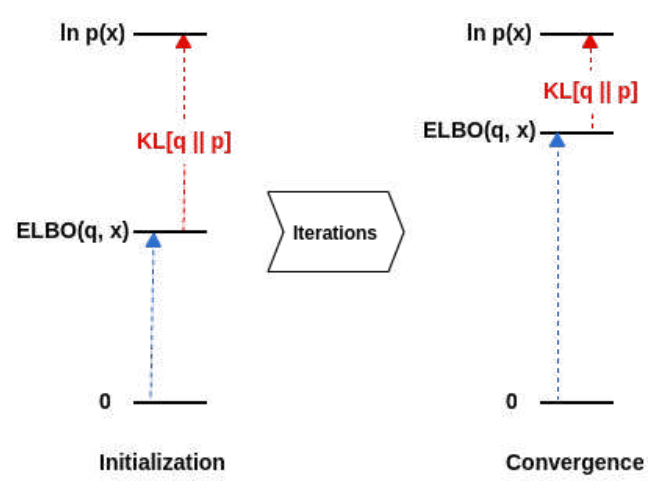
\includegraphics[width=0.4\textwidth]{Immagini/Screenshot 2026-11-15 124421.png}
\end{figure}

\begin{osservazione}[Due KL diverse]
Nelle formule compaiono
$\DKL[q(\mathbf{z}\mid\mathbf{x})\|p(\mathbf{z}\mid\mathbf{x})]$ e
$\DKL[q(\mathbf{z}\mid\mathbf{x})\|p(\mathbf{z})]$. La prima è l'errore di
approssimazione rispetto alla vera posterior e compare solo nell'identità. La
seconda confronta $q$ con la prior ed è il termine di regolarizzazione dentro la
ELBO.
\end{osservazione}

%---------------------------------------------------------------------
\subsection{Il Variational Autoencoder}
%---------------------------------------------------------------------

\subsubsection{Idea}
Un \textbf{VAE} è un autoencoder addestrato a massimizzare la ELBO:
\[
\boxed{
\mathcal{L}_{\mathrm{ELBO}}(\mathbf{x})
=\E_{\mathbf{z}\sim q_\phi(\mathbf{z}\mid\mathbf{x})}[\log p_\theta(\mathbf{x}\mid\mathbf{z})]
-\DKL[q_\phi(\mathbf{z}\mid\mathbf{x})\|p(\mathbf{z})]
}
\]
con $\phi$ parametri dell'encoder e $\theta$ parametri del decoder.

\textbf{Differenza rispetto a un autoencoder standard:} l'encoder non
restituisce un vettore latente deterministico, ma i parametri di una
distribuzione, da cui si estrae il codice.
\[
\mathbf{x}\longrightarrow\text{Encoder}\longrightarrow q_\phi(\mathbf{z}\mid\mathbf{x})
\longrightarrow\mathbf{z}\longrightarrow\text{Decoder}\longrightarrow\widetilde{\mathbf{x}}
\]

\begin{figure}[H]
\centering
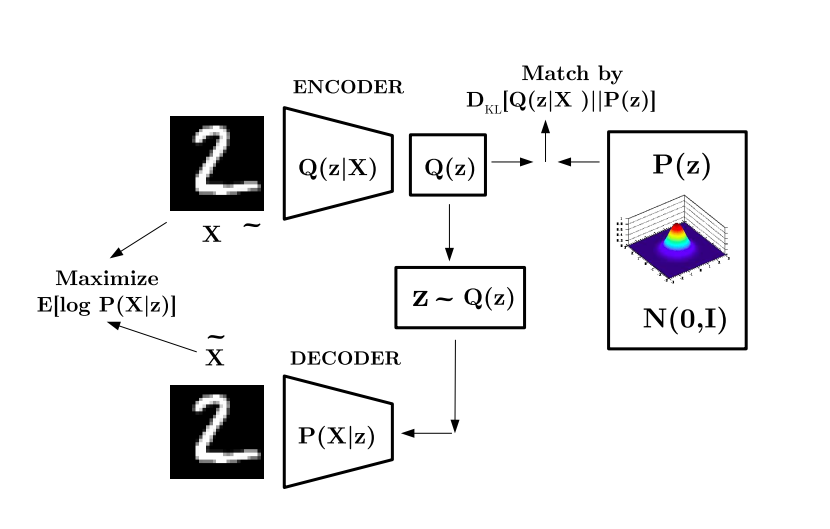
\includegraphics[width=0.5\textwidth]{Immagini/Screenshot 2026-11-15 173716.png}
\end{figure}

\subsubsection{Encoder}
L'encoder realizza la distribuzione approssimata
$q_\phi(\mathbf{z}\mid\mathbf{x})$.

Dato $\mathbf{x}$ la rete calcola:
\[
f_{\mathrm{ENC}}(\mathbf{x};\phi)=[\mu(\mathbf{x}),\sigma^2(\mathbf{x})]
\]
che sono i parametri di una Gaussiana:
\[
\boxed{q_\phi(\mathbf{z}\mid\mathbf{x})=\Normal\big(\mathbf{z}\mid\mu(\mathbf{x}),\sigma^2(\mathbf{x})\big)}
\]
\begin{itemize}
    \item $\mu(x)$ è il vettore delle medie;
    \item $\sigma^2(x)$ è il vettore delle varianze;
    \item $z$ è il vettore latente campionato dalla distribuzione.
\end{itemize}
Se lo spazio latente ha dimensione $d$, allora $\mu(x)$ e $\sigma^2(x)$ contengono normalmente $d$ valori ciascuno.
Nel caso usuale di una Gaussiana con covarianza diagonale, ogni dimensione latente ha una propria media 
e una propria varianza.

\textbf{Punto importante:} l'encoder non decide un solo punto $z$ in modo deterministico. Descrive una 
distribuzione di possibili codici latenti. Il campionamento da tale distribuzione introduce variabilità 
nella rappresentazione.


\subsubsection{Decoder}
Il decoder realizza la distribuzione condizionata:
\[
p_\theta(x\mid z).
\]

Riceve un campione $z$ prodotto dall'encoder e genera una ricostruzione, indicata con $\widetilde{x}$:
\[
\boxed{
\widetilde{x}=g_{\mathrm{DEC}}(z;\theta),
\qquad
z\sim q_\phi(z\mid x)
}
\]

La ricostruzione deve essere il più possibile simile all'input originale $x$.

Il termine di ricostruzione della ELBO è:
\[
\E_{z\sim q_\phi(z\mid x)}
[\log p_\theta(x\mid z)].
\]

Massimizzare questo termine significa rendere elevata la probabilità che il decoder assegna al dato originale,
 condizionatamente al codice latente.

Nelle slide viene indicato che, in pratica, si può minimizzare la \textbf{Mean Squared Error (MSE)} tra input
e ricostruzione:
\[
\boxed{
\mathrm{MSE}(x,\widetilde{x})
=
\frac{1}{n}\sum_{i=1}^{n}(x_i-\widetilde{x}_i)^2
}
\]

La MSE penalizza gli errori quadratici tra i valori originali e quelli ricostruiti. 
Minimizzarla favorisce ricostruzioni vicine all'input.
\begin{osservazione}[Perché la MSE]
Con una likelihood gaussiana a varianza fissata, minimizzare la MSE equivale,
a meno di costanti e fattori di scala, a massimizzare la log-verosimiglianza. La
likelihood giusta dipende dal tipo di dato.
\end{osservazione}

\subsubsection{Regolarizzazione e prior}
La prior è scelta da chi progetta il modello. Spesso viene scelta la
Gaussiana standard:
\[
\boxed{p(\mathbf{z})=\Normal(\mathbf{z}\mid 0,I)}
\]
Il termine $\DKL[q_\phi(\mathbf{z}\mid\mathbf{x})\|p(\mathbf{z})]$ misura quanto
l'encoder si discosta dalla prior. Minimizzarlo evita che il modello metta ogni
dato in regioni latenti arbitrarie e isolate: lo spazio latente resta regolare,
ed è quello da cui poi si estraggono codici per generare.

\textbf{KL in forma chiusa.} Quando sia la posterior approssimata sia la prior sono Gaussiane, la KL può essere calcolata con una formula chiusa, senza dover stimare numericamente l'integrale.

Nel caso comune:
\[
q_\phi(z\mid x)
=
\Normal\big(\mu(x),\operatorname{diag}(\sigma^2(x))\big),
\qquad
p(z)=\Normal(0,I),
\]
la divergenza è:
\[
\boxed{
\DKL[q_\phi(z\mid x)\|p(z)]
=
\frac{1}{2}\sum_{j=1}^{d}
\left(
\mu_j(x)^2+\sigma_j(x)^2
-\log\sigma_j(x)^2-1
\right)
}
\]
È piccola quando le medie sono vicine a $0$ e le varianze vicine a $1$, cioè quando 
la distribuzione dell'encoder è vicina alla Gaussiana standard.

\subsubsection{I due termini insieme}
\[
\mathcal{L}_{\mathrm{ELBO}}(\mathbf{x})=
\underbrace{\E_{q_\phi}[\log p_\theta(\mathbf{x}\mid\mathbf{z})]}_{\text{ricostruzione}}
-\underbrace{\DKL[q_\phi(\mathbf{z}\mid\mathbf{x})\|p(\mathbf{z})]}_{\text{regolarizzazione}}
\]
\begin{itemize}
    \item il termine di ricostruzione spinge il modello a conservare nel codice $z$ le informazioni necessarie per ricostruire $x$;
    \item il termine di regolarizzazione spinge la distribuzione latente verso la prior, rendendo lo spazio latente più regolare.
\end{itemize}

\textbf{QUINDI:} massimizzare la ELBO è un compromesso tra ricostruzioni accurate
e uno spazio latente ben organizzato.

%---------------------------------------------------------------------
\subsection{Reparameterization trick}
%---------------------------------------------------------------------

\textbf{Il problema.} Per passare dall'encoder al decoder dobbiamo estrarre un campione:
\[
z\sim
\Normal\big(\mu(x),\sigma^2(x)\big).
\]

Il problema è che il campionamento è un'operazione casuale. Se lo rappresentiamo come un'operazione separata tra encoder e decoder, 
il gradiente della funzione obiettivo non può essere propagato in modo diretto attraverso quel passaggio verso i parametri $\mu(x)$ e $\sigma(x)$.

Questo è un problema perché vogliamo addestrare encoder e decoder con la backpropagation e la discesa del gradiente.

\textbf{L'idea.} Il \textit{reparameterization trick} riscrive il campionamento in modo da separare:
\begin{itemize}
    \item la componente casuale, indipendente dai parametri appresi;
    \item la trasformazione deterministica che utilizza i parametri prodotti dall'encoder.
\end{itemize}
Invece di campionare direttamente:
\[
z\sim\Normal\big(\mu(x),\sigma^2(x)\big),
\]
si estrae prima un vettore casuale dalla Gaussiana standard:
\[
\boxed{
\epsilon\sim\Normal(0,I)
}
\]

Poi si costruisce $z$ attraverso:
\[
\boxed{
z=\mu(x)+\epsilon\odot\sigma(x)
}
\]
dove $\odot$ indica il prodotto elemento per elemento e $\sigma(x)$ è il vettore delle deviazioni standard:
\[
\sigma(x)=\sqrt{\sigma^2(x)}.
\]

La variabile $\epsilon$ contiene il rumore casuale, mentre $\mu(x)$ e $\sigma(x)$ sono prodotte dall'encoder.

% \textbf{Perché funziona.} Se $\epsilon\sim\Normal(0,I)$,
% \[
% \E[\mathbf{z}]=\mu(\mathbf{x})+\sigma(\mathbf{x})\odot\E[\epsilon]=\mu(\mathbf{x}),
% \qquad
% \operatorname{Var}(z_j)=\sigma_j(\mathbf{x})^2\operatorname{Var}(\epsilon_j)=\sigma_j(\mathbf{x})^2.
% \]
% Quindi $\mathbf{z}\sim\Normal(\mu(\mathbf{x}),\operatorname{diag}(\sigma^2(\mathbf{x})))$,
% come richiesto.

\textbf{Vantaggio.} Il rumore $\boldsymbol{\epsilon} \sim \mathcal{N}(\mathbf{0}, \mathbf{I})$ viene campionato da una 
distribuzione fissa che non dipende dai parametri $\phi$ dell'encoder. Una volta estratto, 
viene trattato come un semplice input aggiuntivo costante.

La dipendenza dai parametri appresi è ora esplicita e differenziabile:
\[
    \mathbf{z} = \boldsymbol{\mu}_\phi(\mathbf{x}) + \boldsymbol{\sigma}_\phi(\mathbf{x}) \odot \boldsymbol{\epsilon}.
\]

Di conseguenza, il gradiente può attraversare $\mathbf{z}$ e raggiungere i parametri dell'encoder tramite le normali
 derivate parziali (elemento per elemento):
\[
    \frac{\partial \mathbf{z}}{\partial \boldsymbol{\mu}_\phi(\mathbf{x})} = \mathbf{1},
    \qquad
    \frac{\partial \mathbf{z}}{\partial \boldsymbol{\sigma}_\phi(\mathbf{x})} = \boldsymbol{\epsilon}.
\]

In parole semplici: il campionamento casuale non viene eliminato, ma viene spostato fuori dalla rete dentro 
$\boldsymbol{\epsilon}$; in questo modo $\mathbf{z}$ diventa una normale operazione matematica (somma e prodotto)
 attraverso cui la backpropagation può passare senza bloccarsi.

\begin{center}
\renewcommand{\arraystretch}{1.35}
\begin{tabular}{|p{6.9cm}|p{6.9cm}|}
\hline
\textbf{Campionamento diretto} & \textbf{Riparametrizzato} \\
\hline
L'encoder produce $\mu$ e $\sigma^2$. & L'encoder produce $\mu$ e $\sigma^2$. \\
\hline
Si estrae $\mathbf{z}\sim\Normal(\mu,\sigma^2)$. & Si estrae $\epsilon\sim\Normal(0,I)$. \\
\hline
L'operazione casuale ostacola il gradiente. & $\mathbf{z}=\mu+\sigma\odot\epsilon$ è differenziabile in $\mu$ e $\sigma$. \\
\hline
\end{tabular}
\end{center}

%---------------------------------------------------------------------
\subsection{Training e generazione}
%---------------------------------------------------------------------

\textbf{Un passo di addestramento:}
\begin{enumerate}
  \item $\mathbf{x}$ entra nell'encoder, che calcola $\mu(\mathbf{x})$ e $\sigma^2(\mathbf{x})$;
  \item si estrae $\epsilon\sim\Normal(0,I)$ e si costruisce
        $\mathbf{z}=\mu(\mathbf{x})+\sigma(\mathbf{x})\odot\epsilon$;
  \item il decoder produce $\widetilde{\mathbf{x}}$;
  \item termine di ricostruzione tra $\mathbf{x}$ e $\widetilde{\mathbf{x}}$
        (nelle slide, la MSE);
  \item KL tra $q_\phi(\mathbf{z}\mid\mathbf{x})$ e $p(\mathbf{z})$;
  \item si massimizza la ELBO, o si minimizza la sua versione cambiata di segno.
\end{enumerate}

\textbf{Generazione.} Dopo l'addestramento la regolarizzazione ha avvicinato le
distribuzioni latenti alla prior, quindi si può campionare dalla prior e
passare il codice al decoder, senza encoder e senza dati osservati:
\[
\mathbf{z}\sim p(\mathbf{z})\qquad\longrightarrow\qquad\widetilde{\mathbf{x}}\sim p_\theta(\mathbf{x}\mid\mathbf{z}).
\]

% \begin{figure}[H]
% \centering
% \includegraphics[width=0.6\textwidth]{Immagini/Screenshot 2026-11-14 VAE campioni.png}
% \caption{Esempi di campioni generati da un VAE.}
% \end{figure}

%---------------------------------------------------------------------
\subsection{Riepilogo}
%---------------------------------------------------------------------

\begin{importante}[Da saper dire a voce]
Un modello generativo impara $p(\mathbf{x})$ per generare nuovi dati. Con una
variabile latente $\mathbf{z}$ si ha
$p(\mathbf{x})=\int p(\mathbf{x}\mid\mathbf{z})p(\mathbf{z})\,d\mathbf{z}$, che è
intrattabile; Monte Carlo dalla prior funziona male perché la prior non dipende
da $\mathbf{x}$. L'inferenza variazionale approssima la posterior con una
$q(\mathbf{z}\mid\mathbf{x})$ e, dall'identità
$\log p(\mathbf{x})=\DKL[q\|p(\mathbf{z}\mid\mathbf{x})]+\mathrm{ELBO}$, massimizzare
la ELBO equivale a minimizzare quella KL. La ELBO ha un termine di ricostruzione
e un termine KL verso la prior. Il VAE realizza $q$ con un encoder che produce
$\mu$ e $\sigma^2$ e $p(\mathbf{x}\mid\mathbf{z})$ con un decoder; il
reparameterization trick, $\mathbf{z}=\mu+\sigma\odot\epsilon$, permette di
propagare il gradiente attraverso il campionamento.
\end{importante}

\begin{itemize}
    \item \textbf{Generative modeling:} imparare una distribuzione $p(x)$ per generare nuovi dati simili a quelli osservati.
    \item \textbf{Variabile latente $z$:} fattore nascosto che contribuisce a spiegare il dato osservato $x$.
    \item \textbf{Modello latente:}
    \[
    p(x)=\int p(x\mid z)p(z)\,dz.
    \]
    \item \textbf{Problema:} l'integrale può essere intrattabile; Monte Carlo lo approssima con campioni dalla prior, ma il campionamento può essere inefficiente per una specifica osservazione.
    \item \textbf{Inferenza variazionale:} approssimare la posterior $p(z\mid x)$ con una distribuzione più semplice $q(z\mid x)$.
    \item \textbf{ELBO:}
    \[
    \mathrm{ELBO}
    =
    \E_q[\log p(x\mid z)]
    -
    \DKL[q(z\mid x)\|p(z)].
    \]
    \item \textbf{VAE:} encoder probabilistico che produce media e varianza, campionamento di $z$ e decoder che ricostruisce il dato.
    \item \textbf{Ricostruzione:} favorisce un codice latente che conservi le informazioni necessarie per ricostruire $x$.
    \item \textbf{Regolarizzazione:} avvicina $q(z\mid x)$ alla prior, tipicamente $\Normal(0,I)$.
    \item \textbf{Reparameterization trick:}
    \[
    \epsilon\sim\Normal(0,I),
    \qquad
    z=\mu(x)+\sigma(x)\odot\epsilon,
    \]
    che consente di propagare il gradiente attraverso la trasformazione usata per ottenere il codice latente.
\end{itemize}

%=====================================================================
\section{Generative Adversarial Networks}
%=====================================================================

%---------------------------------------------------------------------
\subsection{Perché le GAN}
%---------------------------------------------------------------------

Le \textbf{Generative Adversarial Networks (GAN)} sono un approccio generativo
alternativo ai VAE e ai VQ-VAE. I modelli come il VAE usano variabili latenti
$\mathbf{z}$, ottimizzano un limite inferiore della log-verosimiglianza (la
ELBO) e possono produrre ricostruzioni sfocate (\emph{blurry}).

Le GAN cambiano impostazione:
\begin{itemize}
  \item non modellano una densità esplicita facile da valutare;
  \item imparano a mappare direttamente rumore $\mathbf{z}\sim p(\mathbf{z})$
        nella distribuzione dei dati reali;
  \item si addestrano con una competizione tra due reti, infatti il generator
  cerca di produrre risultati più realistici mentre il discriminatore cerca di 
  riconoscere meglio i dati artificiali. Idealmente i dati generati diventano indistinguibili
\end{itemize}
\[
\boxed{\mathbf{z}\sim p(\mathbf{z})\quad\longrightarrow\quad G(\mathbf{z})\ \text{simile ai dati reali}}
\]
Il generatore trasforma un vettore casuale in un dato sintetico, ad esempio
un'immagine.

\begin{figure}[H]
\centering
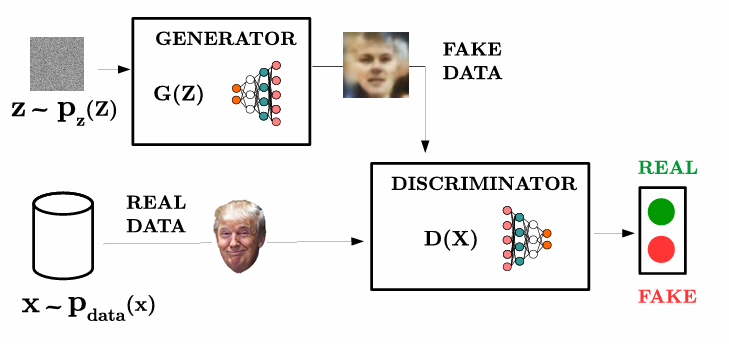
\includegraphics[width=0.5\textwidth]{Immagini/Screenshot 2026-11-17 222926.png}
\end{figure}

\begin{osservazione}[Densità implicita]
Una GAN genera campioni ma non dà una formula semplice per $p(\mathbf{x})$, cioè
la probabilità di una specifica osservazione. Il processo di generazione si
impara attraverso il confronto con il discriminatore.
\end{osservazione}

\subsubsection{Generator}
Riceve un vettore casuale da una distribuzione semplice (\emph{noise prior}) e
lo trasforma in un campione con una rete neurale:
\[
\mathbf{z}\sim p(\mathbf{z}),\qquad
\boxed{\mathbf{x}_{\mathrm{fake}}=G_{\theta_G}(\mathbf{z})}
\]
$\theta_G$ sono i parametri del generatore. Per le immagini, $G$ trasforma il
rumore in un'immagine sintetica.

\subsubsection{Discriminator}
Riceve un campione $\mathbf{x}$ e restituisce la probabilità che provenga dal
dataset reale:
\[
\boxed{D_{\theta_D}(\mathbf{x})\in[0,1]}
\]
\begin{itemize}
  \item $D(\mathbf{x})\approx 1$: il campione è giudicato reale;
  \item $D(\mathbf{x})\approx 0$: il campione è giudicato generato (fake).
\end{itemize}
Si addestra sia su dati reali sia su dati prodotti da $G$.

\textbf{QUINDI:} Il discriminatore deve dare un valore alto ai dati reali e basso a quelli
generati. Il generatore vuole alzare il punteggio dei propri campioni.

%---------------------------------------------------------------------
\subsection{Funzione obiettivo: il gioco minimax}
%---------------------------------------------------------------------

Le due reti hanno obiettivi opposti:
\[
\min_{\theta_G}\max_{\theta_D}V(D,G)
=\E_{\mathbf{x}\sim p_{\mathrm{data}}}\big[\log D_{\theta_D}(\mathbf{x})\big]
+\E_{\mathbf{z}\sim p(\mathbf{z})}\big[\log\big(1-D_{\theta_D}(G_{\theta_G}(\mathbf{z}))\big)\big]
\]

\subsubsection{Obiettivo del discriminatore}
Massimizza $V$ rispetto a $\theta_D$:
\[
\max_{\theta_D}\Big\{\E_{\mathbf{x}\sim p_{\mathrm{data}}}\log D(\mathbf{x})
+\E_{\mathbf{z}\sim p(\mathbf{z})}\log\big(1-D(G(\mathbf{z}))\big)\Big\}
\]
cioè $D(\mathbf{x})\to 1$ sui dati reali e $D(G(\mathbf{z}))\to 0$ su quelli
generati: classificare correttamente real e fake.

\subsubsection{Obiettivo del generatore}
Minimizza la stessa funzione rispetto a $\theta_G$. Il primo termine non dipende
da $G$, quindi resta
\[
\boxed{\min_{\theta_G}\E_{\mathbf{z}\sim p(\mathbf{z})}\big[\log\big(1-D(G(\mathbf{z}))\big)\big]}
\]
Per minimizzarlo il generatore rende $D(G(\mathbf{z}))$ vicino a 1: induce il
discriminatore a classificare come reali i campioni generati.

\textbf{QUINDI:}
\begin{center}
\renewcommand{\arraystretch}{1.35}
\begin{tabular}{|p{2.9cm}|p{5.5cm}|p{5.5cm}|}
\hline
 & \textbf{Discriminator} & \textbf{Generator} \\
\hline
Input & dati reali e generati & rumore $\mathbf{z}$ \\
\hline
Obiettivo & distinguere real e fake & produrre campioni realistici \\
\hline
Output desiderato & $D(\mathbf{x})\to1$, $D(G(\mathbf{z}))\to0$ & $D(G(\mathbf{z}))\to1$ \\
\hline
Ottimizzazione & massimizza $V(D,G)$ & minimizza $V(D,G)$ \\
\hline
\end{tabular}
\end{center}
Il generatore non riceve un'immagine da copiare: riceve dal discriminatore un
feedback su quanto i suoi campioni somigliano ai dati reali.

%---------------------------------------------------------------------
\subsection{Addestramento alternato}
%---------------------------------------------------------------------

Le due reti si aggiornano a turno.
\begin{enumerate}
  \item \textbf{Gradient ascent sul discriminatore.} Si aggiorna $\theta_D$ per
        massimizzare
        $\E_{\mathbf{x}}\log D(\mathbf{x})+\E_{\mathbf{z}}\log(1-D(G(\mathbf{z})))$,
        con $G$ fisso.
  \item \textbf{Gradient descent sul generatore.} Si aggiorna $\theta_G$ per
        minimizzare $\E_{\mathbf{z}}[\log(1-D(G(\mathbf{z})))]$, con $D$ fisso.
\end{enumerate}
I due passi si ripetono. L'addestramento è dinamico: quando una rete migliora,
cambia il problema che l'altra deve risolvere.

%---------------------------------------------------------------------
\subsection{Vanishing gradient nel generatore}
%---------------------------------------------------------------------

Con l'obiettivo minimax il generatore minimizza
\[
L_G^{\mathrm{minimax}}=\E_{\mathbf{z}\sim p(\mathbf{z})}\big[\log\big(1-D(G(\mathbf{z}))\big)\big].
\]
All'inizio i campioni sono poco realistici, il discriminatore li riconosce
facilmente e $D(G(\mathbf{z}))\approx 0$. In questo caso il logaritmo è vicino a
zero e il gradiente che arriva al generatore è molto piccolo: il generatore
riceve un segnale debole proprio quando ne avrebbe più bisogno.

\begin{osservazione}[Perché il gradiente è piccolo (non nelle slide)]
Se $D=\sigma(a)$, con $a$ il valore prima della sigmoide, allora
\[
\frac{\partial}{\partial a}\log(1-\sigma(a))=-\sigma(a),
\qquad
\frac{\partial}{\partial a}\log\sigma(a)=1-\sigma(a).
\]
Quando $D(G(\mathbf{z}))\approx0$ il primo gradiente è vicino a zero, il secondo
vicino a 1. È questa la ragione del cambio di obiettivo.
\end{osservazione}

\textbf{Soluzione: obiettivo non saturante.} Invece di minimizzare
$\log(1-D(G(\mathbf{z})))$, il generatore massimizza
\[
\boxed{\max_{\theta_G}\E_{\mathbf{z}\sim p(\mathbf{z})}\big[\log D_{\theta_D}(G_{\theta_G}(\mathbf{z}))\big]}
\]
Lo scopo è lo stesso ($D(G(\mathbf{z}))\to1$), ma il gradiente è più forte
all'inizio dell'addestramento.

\begin{center}
\renewcommand{\arraystretch}{1.35}
\begin{tabular}{|p{3.2cm}|p{9.6cm}|}
\hline
\textbf{Minimax} & $\displaystyle\min_{\theta_G}\E_{\mathbf{z}}[\log(1-D(G(\mathbf{z})))]$ \\
\hline
\textbf{Non saturante} & $\displaystyle\max_{\theta_G}\E_{\mathbf{z}}[\log D(G(\mathbf{z}))]$ \\
\hline
\end{tabular}
\end{center}

%---------------------------------------------------------------------
\subsection{Algoritmo di training}
%---------------------------------------------------------------------

Si usano minibatch di dimensione $m$. Per ogni aggiornamento del generatore si
fanno $k$ aggiornamenti del discriminatore ($k$ è un iperparametro; nei
loro esperimenti le slide usano $k=1$, la scelta meno costosa).

\textbf{Passo 1: discriminatore.}
\begin{enumerate}
  \item minibatch di rumore $\{\mathbf{z}^{(1)},\dots,\mathbf{z}^{(m)}\}\sim p(\mathbf{z})$;
  \item minibatch di dati reali $\{\mathbf{x}^{(1)},\dots,\mathbf{x}^{(m)}\}\sim p_{\mathrm{data}}(\mathbf{x})$;
  \item gradient ascent su $\theta_D$:
  \[
  \boxed{
  \nabla_{\theta_D}\frac1m\sum_{i=1}^{m}\Big[\log D(\mathbf{x}^{(i)})+\log\big(1-D(G(\mathbf{z}^{(i)}))\big)\Big]
  }
  \]
\end{enumerate}

\textbf{Passo 2: generatore.}
\begin{enumerate}
  \item nuovo minibatch di rumore $\{\mathbf{z}^{(1)},\dots,\mathbf{z}^{(m)}\}\sim p(\mathbf{z})$;
  \item gradient descent su $\theta_G$:
  \[
  \boxed{
  \nabla_{\theta_G}\frac1m\sum_{i=1}^{m}\log\big(1-D(G(\mathbf{z}^{(i)}))\big)
  }
  \]
\end{enumerate}
Gli aggiornamenti usano i normali metodi basati sul gradiente (le slide citano
anche il momentum). L'algoritmo riporta la loss minimax originale, ma nelle
implementazioni si usa di solito l'obiettivo non saturante.

\textbf{Generazione.} Dopo l'addestramento il discriminatore non serve più, ha
fornito il segnale durante il training:
\[
\mathbf{z}\sim p(\mathbf{z}),\qquad \mathbf{x}_{\mathrm{fake}}=G(\mathbf{z}).
\]

%---------------------------------------------------------------------
\subsection{Deep Convolutional GAN (DCGAN)}
%---------------------------------------------------------------------

La DCGAN usa un'architettura convoluzionale sia nel generatore sia nel
discriminatore. Migliora la qualità delle immagini e la stabilità
dell'addestramento, perché le convoluzioni sfruttano le relazioni tra pixel
vicini e le feature gerarchiche.

\textbf{Interpolazione nello spazio latente.} Dati due vettori latenti
$\mathbf{z}_1$ e $\mathbf{z}_2$:

Agli estremi si ottengono $\mathbf{z}_1$ e $\mathbf{z}_2$; per valori intermedi
il generatore produce immagini intermedie. Se lo spazio latente è ben appreso,
le caratteristiche visive cambiano in modo graduale,
la modifica avviene nello spazio latente e il generatore la traduce in una
variazione dell'immagine.

%---------------------------------------------------------------------
\subsection{Evoluzione delle GAN} 
%---------------------------------------------------------------------
\textbf{DA CHEIDERE MA PER ME SI PUO SALTARE FINO A PRO E CONTRO}
Sono state proposte nel tempo diverse loss e architetture per migliorare la
qualità dei campioni e lar stabilità.

\begin{itemize}
  \item \textbf{LSGAN} (Mao et al., 2017): sostituisce la loss logaritmica con
        una loss ai minimi quadrati, per avere gradienti migliori.
  \item \textbf{Wasserstein GAN} (Arjovsky et al., 2017): cambia la misura della
        differenza tra distribuzione reale e generata, per avere un segnale di
        apprendimento più informativo e più stabile.
  \item \textbf{Improved WGAN} (Gulrajani et al., 2017): aggiunge accorgimenti
        per addestrare meglio la Wasserstein GAN.
  \item \textbf{CycleGAN} (Zhu et al., 2017): traduzione immagine--immagine
        (\emph{image-to-image translation}) con dati \emph{unpaired}, cioè senza
        coppie di immagini corrispondenti (da Monet a fotografia, da zebra a
        cavallo). \emph{Cycle-consistent}: se si trasforma un'immagine nel
        dominio di arrivo e poi di nuovo in quello di partenza, si deve
        recuperare l'originale.
\end{itemize}

\subsubsection{Progressive GAN}
L'addestramento è progressivo: generatore e discriminatore partono a bassa
risoluzione e si aggiungono livelli man mano, fino a risoluzioni alte (nelle
slide da $4\times4$ a $1024\times1024$). Il modello impara prima le strutture
generali e poi i dettagli. I livelli già presenti restano addestrabili.

\subsubsection{StyleGAN}
StyleGAN (versioni 1, 2 e 3) usa un generatore basato sullo \emph{stile}, che
permette un controllo più fine degli attributi dell'immagine. Il latente non
entra direttamente nel generatore: una rete di mapping lo porta prima in uno
spazio intermedio $W$,
\[
\mathbf{z}\longrightarrow\mathbf{w}=f(\mathbf{z}),
\]
e $\mathbf{w}$ controlla i livelli della rete di sintesi.
\begin{itemize}
  \item \textbf{AdaIN} (Adaptive Instance Normalization): modula le attivazioni
        delle feature map in funzione dello stile.
  \item \textbf{Rumore esplicito:} immagini a un canale di rumore gaussiano non
        correlato, aggiunte alle feature map con fattori di scala appresi per
        canale. Danno i dettagli stocastici locali, che non dipendono solo dal
        latente globale.
\end{itemize}

\textbf{Controllo degli attributi a più scale.} Si possono combinare gli stili
di due codici sorgente A e B, trasferendo da B ad A solo alcuni livelli:
\begin{itemize}
  \item \textbf{Coarse} ($4^2$--$8^2$): posa, forma generale del volto,
        acconciatura, occhiali;
  \item \textbf{Middle} ($16^2$--$32^2$): tratti del volto, occhi, dettagli
        dell'acconciatura;
  \item \textbf{Fine} ($64^2$--$1024^2$): schema dei colori e microstruttura.
\end{itemize}

\textbf{FID} (Fréchet Inception Distance). Confronta le distribuzioni delle
feature, estratte da una rete Inception, delle immagini reali e di quelle generate:
\[
\boxed{\text{FID più bassa}\ \Longrightarrow\ \text{risultato migliore}}
\]
\begin{center}
\renewcommand{\arraystretch}{1.25}
\begin{tabular}{|l|c|c|}
\hline
\textbf{Configurazione} & \textbf{CelebA-HQ} & \textbf{FFHQ} \\
\hline
Baseline Progressive GAN & 7.79 & 8.04 \\
\hline
Tuning (incl. bilinear up/down) & 6.11 & 5.25 \\
\hline
Mapping e styles & 5.34 & 4.85 \\
\hline
Rimozione input tradizionale & 5.07 & 4.88 \\
\hline
Aggiunta ingressi di rumore & 5.06 & 4.42 \\
\hline
Mixing regularization & 5.17 & 4.40 \\
\hline
\end{tabular}
\end{center}
Le modifiche influenzano la qualità misurata dalla FID, ma non ogni singola
modifica migliora il risultato su entrambi i dataset.

%---------------------------------------------------------------------
\subsection{Vantaggi e limiti}
%---------------------------------------------------------------------

\textbf{Vantaggi.}
\begin{itemize}
  \item \textbf{Backpropagation:} le due reti si addestrano con aggiornamenti
        basati sul gradiente;
  \item \textbf{Loss appresa:} il segnale per il generatore dipende dalla
        capacità del discriminatore di distinguere real e fake, non da una loss
        di ricostruzione scelta a mano;
  \item \textbf{Nessun MCMC:} per generare basta estrarre rumore e passarlo al
        generatore.
\end{itemize}

\textbf{Svantaggi.}
\begin{itemize}
  \item \textbf{Training difficile e instabile,} più di altri modelli
        generativi, e da controllare con attenzione;
  \item \textbf{Valutazione difficile:} non esiste una metrica unica. Qualità
        visiva e copertura della distribuzione sono aspetti distinti.
\end{itemize}

\begin{osservazione}[Mode collapse (non nelle slide)]
Il generatore può produrre solo una parte dei modi della distribuzione reale,
ripetendo campioni simili.
\end{osservazione}

\subsubsection{Confronto VAE--GAN}
\begin{center}
\renewcommand{\arraystretch}{1.35}
\begin{tabular}{|p{2.5cm}|p{5.6cm}|p{5.6cm}|}
\hline
 & \textbf{VAE} & \textbf{GAN} \\
\hline
Idea & encoder probabilistico e decoder & competizione tra generatore e discriminatore \\
\hline
Latente & $\mathbf{z}\sim q_\phi(\mathbf{z}\mid\mathbf{x})$ in training & $\mathbf{z}\sim p(\mathbf{z})$, rumore in ingresso \\
\hline
Obiettivo & massimizzare la ELBO & gioco minimax \\
\hline
Ricostruzione & il decoder ricostruisce l'input & non serve un percorso di ricostruzione \\
\hline
Densità & modello probabilistico con likelihood & nessuna densità esplicita facile da valutare \\
\hline
Criticità & ricostruzioni sfocate & training instabile, valutazione difficile \\
\hline
\end{tabular}
\end{center}

\begin{importante}[Da saper dire a voce]
Una GAN impara a generare dati con due reti in competizione. Il generatore
$G$ trasforma rumore $\mathbf{z}$ in un campione; il discriminatore $D$ stima la
probabilità che un campione sia reale. Il gioco è
$\min_G\max_D\ \E[\log D(\mathbf{x})]+\E[\log(1-D(G(\mathbf{z})))]$: $D$ vuole
riconoscere i fake, $G$ vuole ingannarlo. Si addestrano alternando i due
aggiornamenti. All'inizio $D(G(\mathbf{z}))\approx0$ e il gradiente del generatore
quasi sparisce, quindi si usa l'obiettivo non saturante
$\max_G\E[\log D(G(\mathbf{z}))]$. Rispetto al VAE non c'è densità esplicita né
ricostruzione, ma l'addestramento è meno stabile.
\end{importante}

\section{Rappresentazioni discrete e VQ-VAE}

\subsection{Discretizzazione}

La \textbf{discretizzazione} è il processo con cui un fenomeno continuo viene diviso in parti distinte. Le slide la 
presentano come un processo cognitivo fondamentale, studiato da secoli in filosofia, scienza e matematica.

\textbf{Punto importante:} Nel machine learning spesso e' necessario trasformare
un fenomeno complesso in simboli o categorie per rendere la sua struttura
più gestibile e possono garantire nei sistemi IA.

\begin{itemize}
  \item \textbf{compressione efficiente};
  \item \textbf{ragionamento simbolico};
  \item \textbf{design modulare}.
\end{itemize}

Molti domini sono per natura discreti:
\begin{itemize}
  \item il \textbf{linguaggio} è una sequenza di simboli discreti (parole, subword, fonemi);
  \item le \textbf{immagini} sono griglie discrete di pixel con valori di colore quantizzati;
  \item \textbf{musica e parlato} sono spesso rappresentati in modo simbolico (note, fonemi).
\end{itemize}

\subsection{Il problema: variabili discrete e gradient descent}

Le reti si ottimizzano con il gradient descent, e hanno la necessita' di essere continue. 
Le scelte discrete non sono differenziabili, e la backpropagation standard non passa attraverso:
\begin{itemize}
  \item \texttt{argmax};
  \item il campionamento da una distribuzione categorica.
\end{itemize}

Alcune \textit{soluzioni}:
\begin{itemize}
  \item i \textbf{VQ-VAE} usano gli \emph{straight-through estimator};
  \item i \textbf{Pixel-RNN} usano un addestramento autoregressivo (teacher forcing, massimizzazione della likelihood);
  \item i gradienti surrogati, come il \textbf{Gumbel-Softmax}.
\end{itemize}

\subsection{Problemi del VAE}

\textbf{Output sfocati e mode collapse.} I VAE tendono a generare output sfocati e poco realistici. Nel 
\emph{mode collapse} il modello genera solo un sottoinsieme dei possibili output, 
ignorando la varietà del training set. 

\textbf{Posterior collapse.} Il posterior variazionale dell'encoder collassa rapidamente verso la prior nelle 
prime fasi dell'addestramento. Quando cio' succede:
\begin{itemize}
  \item le variabili latenti smettono di portare informazione utile sull'input e il decoder impara a ignorarle;
  \item il collasso è spesso \textit{irreversibile} una volta che converge alla prior.
\end{itemize}

\textbf{SOLUZIONI:}
\begin{enumerate}
  \item \textbf{$\beta$-VAE:} introduce un iperparametro $\beta$ che pesa la KL nella ELBO:
  \[
  \boxed{\E_{z \sim q(z \mid x)}\big[\log p(x \mid z)\big] - \beta\, \DKL\big[q(z \mid x) \,\|\, p(z)\big]}
  \]
  \item \textbf{VQ-VAE}.
\end{enumerate}

\subsection{Vector Quantised-VAE (VQ-VAE)}

\subsubsection{Idea}

Il VQ-VAE usa le \textbf{variabili latenti discrete}. 
Usa l'intero spazio latente ed evita il posterior collapse.

\subsubsection{Architettura}

Il VQ-VAE è un autoencoder \emph{standard}, con un encoder e un decoder. A differenza del VAE, lo spazio latente 
non segue una distribuzione gaussiana.

\begin{figure}[H]
\centering
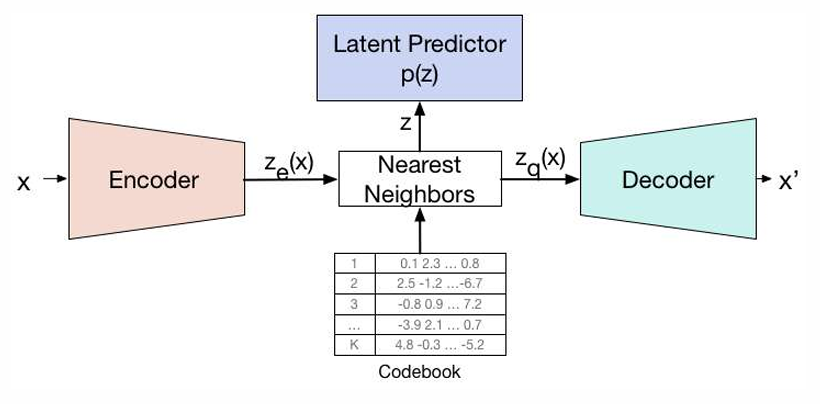
\includegraphics[width=0.5\textwidth]{Immagini/Screenshot 2026-11-21 192259.png}
\end{figure}

Lo spazio latente è definito da una tabella di lookup apprendibile, il \textbf{codebook}:
\[
\boxed{e \in \R^{K \times D}}
\]
\begin{itemize}
  \item $K$ è la dimensione dello spazio latente discreto;
  \item $D$ è la dimensione di ciascun embedding;
  \item ognuno dei $K$ vettori $e_i \in \R^{D}$, $i = 1, \ldots, K$, si apprende con la discesa del gradiente.
\end{itemize}

\textbf{Forward.}
\begin{enumerate}
  \item l'input $x$ passa nell'encoder, che produce un output continuo $z_e(x)$;
  \item i latenti discreti $z$ si calcolano cercando, nello spazio di embedding condiviso, l'embedding più simile a $z_e(x)$:
  \[
  \boxed{q(z = k \mid x) =
  \begin{cases}
  1 & \text{se } k = \argmin_j \|z_e(x) - e_j\|_2, \\
  0 & \text{altrimenti}
  \end{cases}}
  \]
  la distribuzione di proposta è \textbf{deterministica};
  \item l'ingresso del decoder è il vettore di embedding corrispondente:
  \[
  \boxed{z_q(x) = e_k, \qquad k = \argmin_j \|z_e(x) - e_j\|_2}
  \]
  \item il decoder ricostruisce $x'$.
\end{enumerate}

\[
x \longrightarrow \text{Encoder} \longrightarrow z_e(x) \longrightarrow \text{Nearest neighbour} \longrightarrow z_q(x) \longrightarrow \text{Decoder} \longrightarrow x'
\]

L'insieme dei parametri è l'unione dei parametri di encoder, decoder e codebook $e$.

\begin{osservazione}[Esempio numerico]
Con $K = 3$, $D = 2$, $e_1 = (0,0)$, $e_2 = (1,1)$, $e_3 = (-1,2)$ e $z_e = (0.8, 0.6)$, le 
distanze euclidee sono circa $1.0$, $0.45$ e $2.28$. Quindi $k = 2$ e il decoder riceve $z_q = (1,1)$.
\end{osservazione}

\subsection{Apprendimento del VQ-VAE}

\subsubsection{Straight-through estimator}

La pipeline forward è un autoencoder normale con una non linearità particolare, che mappa 
i latenti in un vettore di embedding 1-of-$K$. Questa operazione \textbf{non è differenziabile}: 
\texttt{argmax}, \texttt{round} e \texttt{quantize} rompono il flusso del gradiente.

\textbf{Soluzione.} Si approssimano i gradienti copiando il gradiente dall'ingresso del decoder 
$z_q(x)$ all'uscita dell'encoder $z_e(x)$. In generale lo \textbf{Straight-Through Estimator} (STE) permette di addestrare:
\begin{itemize}
  \item usando l'output discreto nel forward;
  \item facendo backpropagation come se l'operazione fosse l'identità.
\end{itemize}

\[
\boxed{\text{Forward: } z_q = \mathrm{quantize}(z_e) \qquad \text{Backward: } \frac{\partial L}{\partial z_e} \approx \frac{\partial L}{\partial z_q}}
\]

Il trucco si usa anche nei \emph{binary neural gates} (forward come step, backward come sigmoide), 
nella neural architecture search, nel routing e nel pruning.

\begin{figure}[H]
\centering
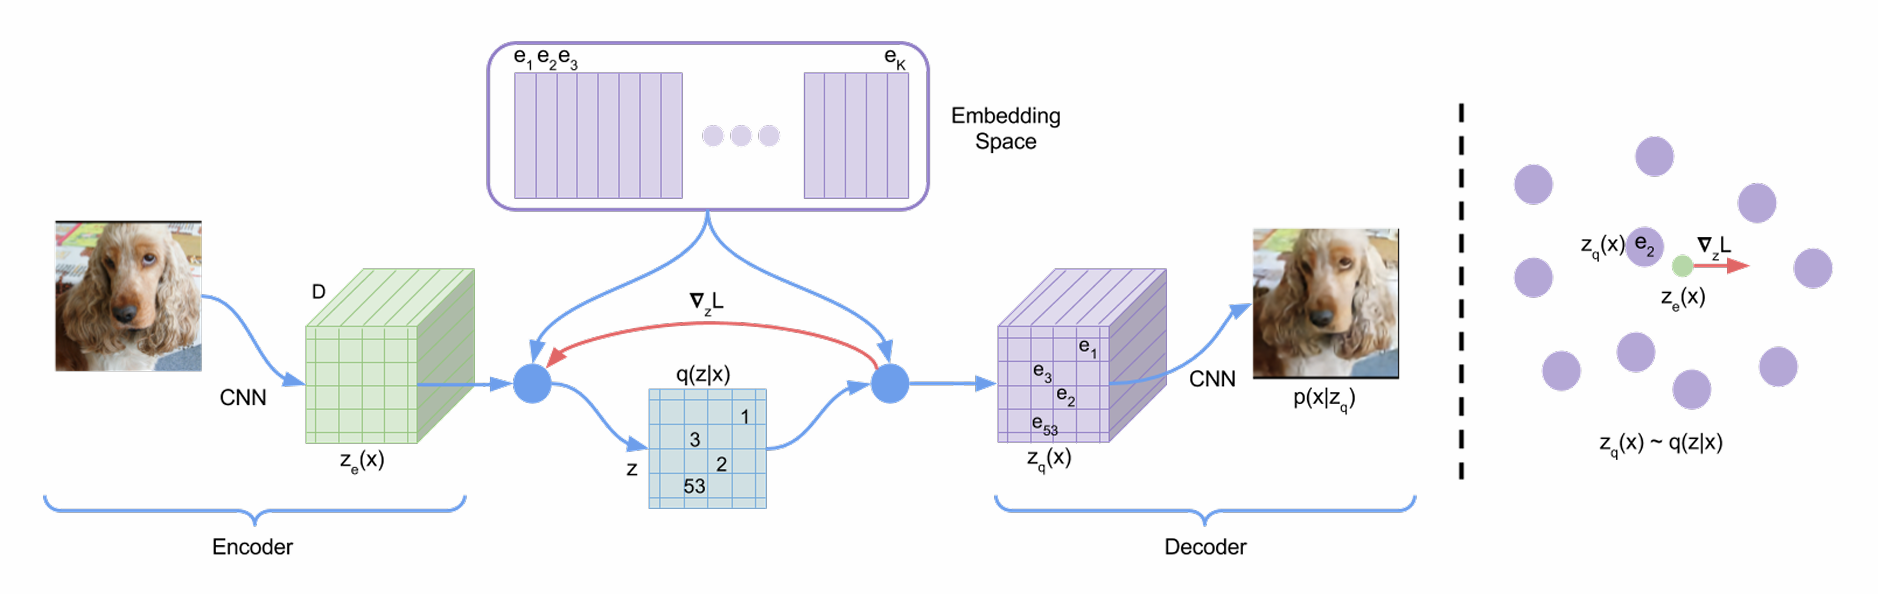
\includegraphics[width=0.8\textwidth]{Immagini/Screenshot 2026-11-21 192315.png}
\end{figure}


\subsubsection{La forma con \texttt{detach}}

Nel VQ-VAE lo STE si implementa così:
\[
\boxed{z_q^{\mathrm{st}} = z_e + \operatorname{detach}(z_q - z_e)}
\]
\begin{itemize}
  \item \textbf{Forward:} $z_q^{\mathrm{st}} = z_q$, quindi la quantizzazione viene eseguita;
  \item \textbf{Backward:} il gradiente passa solo da $z_e$, quindi non è influenzato dalla quantizzazione.
\end{itemize}
In pratica, durante la backpropagation la quantizzazione viene trattata come una funzione identità (\emph{forward as step, backward as identity}):
il gradiente non attraversa il blocco discreto in un flusso continuo, ma ``salta'' direttamente dall'input del decoder $z_q(x)$ all'output dell'encoder $z_e(x)$.



\subsubsection{Funzione obiettivo}

Per effetto dello STE gli embedding $e_i$ non ricevono gradiente dalla loss di ricostruzione. 
Per apprendere lo spazio di embedding il VQ-VAE usa il più semplice algoritmo di dictionary learning, la \textbf{Vector Quantisation} (VQ):
\[
L=\underbrace{\log p(x\mid z_q(x))}_{\text{ricostruzione}}+\underbrace{\|\operatorname{stopgrad}[z_e(x)]-z_q(x)\|_2^2}_{\text{Vector Quantisation (VQ)}}+\beta\,\underbrace{\|z_e(x)-\operatorname{stopgrad}[z_q(x)]\|_2^2}_{\text{commitment}}
\]
$\operatorname{stopgrad}[\cdot]$ è l'operatore di stop gradient: il suo argomento è una costante non
aggiornata durante la backpropagation (in PyTorch si ottiene con \texttt{detach()}).
\begin{enumerate}
  \item \textbf{Reconstruction error:} Misura la qualità della ricostruzione del input a partire
  dall'embedding quantizzato. Aggiorna il decoder e, tramite lo STE,
  contribuisce anche all'aggiornamento dell'encoder fino ad avere $\widehat{x}\approx x$.
  \item \textbf{Vector Quantisation (VQ):} Aggiorna esclusivamente i vettori del codebook ($z_q = e_k$), 
  spostando l'embedding selezionato verso l'output dell'encoder $z_e(x)$; 
  quindi la distanza tra l'uscita dell'encoder e il dizionario diventa più piccola.
  \item \textbf{Commitment term:} Incoraggia l'encoder ($z_e$) a mantenere il proprio output
  vicino al codice scelto, cioè a ``impegnarsi'' verso l'embedding
  selezionato per evitare di saltare da un vettore all altro. Il coefficiente $\beta$ ne regola il peso.

\end{enumerate}

\begin{osservazione}[Perché ogni termine aggiorna solo una parte] \textbf{VEDI DOPO SE LASCIARLO}
Con lo STE il gradiente della ricostruzione passa da $z_q$ a $z_e$ senza toccare il codebook. Servono quindi
altri due termini, e lo stopgrad decide chi viene aggiornato.
\begin{itemize}
  \item Nel termine VQ lo stopgrad è su $z_e$, che per quel termine è una costante: la derivata resta solo
  rispetto a $z_q=e_k$, quindi si muove $e_k$ verso $z_e$.
  \item Nel commitment lo stopgrad è su $z_q$: la derivata resta solo rispetto a $z_e$, quindi si muove
  l'encoder verso $e_k$, e il peso $\beta$ riguarda solo l'encoder.
  \item Il commitment serve perché lo spazio di embedding non ha limiti: se il codebook si aggiorna più
  lentamente dell'encoder, $z_e$ può crescere o oscillare tra codici diversi.
\end{itemize}
\end{osservazione}

Chi ottimizza cosa:
\begin{center}
\renewcommand{\arraystretch}{1.3}
\begin{tabular}{lll}
\hline
\textbf{Termine} & \textbf{Aggiornamento principale} & \textbf{Effetto} \\
\hline
$\mathcal{L}_{\mathrm{rec}}$ & Decoder + encoder via STE & Ricostruire $x$ \\
$\mathcal{L}_{\mathrm{codebook}}$ & Codebook & Avvicinare $e_{k^\star}$ a $z_e$ \\
$\mathcal{L}_{\mathrm{commit}}$ & Encoder & Avvicinare $z_e$ al codice scelto \\
\hline
\end{tabular}
\end{center}

\newpage

\subsubsection{Passo di training}
\begin{enumerate}
  \item input: $x$, encoder $E$, decoder $D$, codebook $\{e_k\}_{k=1}^{K}$;
  \item $z_e \leftarrow E(x)$;  //calcolare l'output continuo dell'encoder
  \item $k \leftarrow \argmin_j \|z_e - e_j\|^2$; //Trovare l'indice del codebook più vicino
  \item $z_q \leftarrow e_k$; //Selezionare l'embedding
  \item $z_q^{\mathrm{st}} \leftarrow z_e + \operatorname{detach}(z_q - z_e)$ (STE);
  \item $\hat{x} \leftarrow D(z_q^{\mathrm{st}})$;
  \item $\Loss_{\mathrm{rec}} \leftarrow \|x - \hat{x}\|^2$;
  \item $\Loss_{\mathrm{codebook}} \leftarrow \|\operatorname{stopgrad}[z_e] - z_q\|^2$;
  \item $\Loss_{\mathrm{commit}} \leftarrow \|z_e - \operatorname{stopgrad}[z_q]\|^2$;
  \item $\Loss \leftarrow \Loss_{\mathrm{rec}} + \Loss_{\mathrm{codebook}} + \beta\, \Loss_{\mathrm{commit}}$;
  \item backpropagation e aggiornamento di modello e codebook.
\end{enumerate}

\subsection{VQ-VAE per la compressione di immagini}

Il VQ-VAE si può usare come \textbf{compressore di immagini appreso}:
\begin{itemize}
  \item l'encoder mappa le immagini in codici latenti discreti;
  \item il decoder ricostruisce l'immagine da quei codici;
  \item gli indici del codebook si possono comprimere ulteriormente con l'\emph{entropy coding} (Huffman, codifica aritmetica).
\end{itemize}

\textbf{Vantaggi.}
\begin{itemize}
  \item apprende feature specifiche del dominio, e a bitrate bassi supera i codec progettati a mano;
  \item genera ricostruzioni visivamente coerenti con meno bit.
\end{itemize}

\subsection{Campionare dal VQ-VAE: il problema della prior}

\textbf{Il problema.} Il VQ-VAE apprende un encoder, un decoder e un codebook di embedding, ma 
\textbf{non apprende una prior} sui codici latenti. Si possono ricostruire gli input, ma non si possono generare facilmente nuovi campioni.

\textbf{Soluzione: learned prior.} Non possiamo campionare direttamente dallo spazio latente discreto 
perché non ne conosciamo la distribuzione. Prima si apprende questa distribuzione con un altro modello
 generativo, poi si campiona dalla prior appresa e si decodifica con il decoder del VQ-VAE.
\begin{enumerate}
  \item si codificano i dati di training, ottenendo sequenze di codici latenti discreti;
  \item si addestra un \textbf{modello generativo} su queste sequenze di codici;
  \item dopo l'addestramento, per generare una singola immagine si campionano nuove sequenze di codici 
  dalla prior appresa, e ogni latente dà la rappresentazione di una singola patch;
  \item si decodificano i codici campionati con il decoder del VQ-VAE.
\end{enumerate}

\textbf{QUINDI:} il VQ-VAE rappresenta e ricostruisce i dati, la prior appresa dice quali sequenze di codici 
sono plausibili. Il modello autoregressivo usato per la prior (PixelCNN) è l'argomento della parte successiva delle slide.

\begin{importante}[Da saper dire a voce]
Il gradiente non passa attraverso le operazioni discrete come \texttt{argmax}. Il VQ-VAE ha un encoder che 
produce $z_e(x)$ e un codebook $e \in \R^{K \times D}$; il decoder riceve il vettore del codebook più 
vicino, $z_q = e_k$ con $k = \argmin_j \|z_e - e_j\|$. Lo straight-through estimator usa il codice discreto nel 
forward e copia il gradiente nel backward ($z_e + \operatorname{detach}(z_q - z_e)$). La loss ha tre termini: 
ricostruzione (decoder ed encoder), Vector Quantisation (aggiorna il codebook) e commitment, con peso $\beta$ (aggiorna l'encoder). 
Evita il posterior collapse e si può usare per comprimere le immagini. Non apprende una prior sui codici, quindi per generare si 
addestra un altro modello generativo sulle sequenze di codici.
\end{importante}

\begin{itemize}
  \item Le rappresentazioni discrete sono utili per simboli,
  compressione e struttura modulare, ma le scelte discrete non
  sono direttamente differenziabili.
  \item Il VQ-VAE codifica l'input in un vettore continuo $z_e$,
  lo quantizza scegliendo l'embedding più vicino nel codebook
  e ricostruisce l'input a partire da $z_q$.
  \item Il codebook contiene $K$ embedding di dimensione $D$.
  \item Lo STE usa il codice discreto nel forward e approssima
  il backward come identità.
  \item La loss contiene reconstruction loss, codebook loss e
  commitment loss.
  \item Il VQ-VAE può comprimere immagini in codici latenti
  discreti e ricostruirle.
  \item Per generare nuovi campioni serve anche una prior appresa
  sui codici latenti; il decoder trasforma i codici campionati
  in nuove immagini.
\end{itemize}

.
\end{document}